\documentclass{whswinvcbook}
\usepackage{whswinvcgsp}

\usepackage[ngerman]{babel} % language selection: english/ngerman
                            % note: delete all output files on language change
\usepackage[utf8]{inputenc} % allow for using umlauts
\usepackage{lipsum}         % provide lorem ipsum ...
\usepackage{siunitx}        % provide SI units
\usepackage{amsfonts}       % Provides hollow R for real numbers, hollow C for complex numbers, etc.
\usepackage{algorithm}      % Provides Border for Pseudocode
\usepackage{algpseudocode}  % Provides Pseudocode
\usepackage{interval}       % Provides proper intervals
\usepackage{listings}       % Provides Source Code Listing
\usepackage{gensymb}        % Provides the degree symbol
\usepackage{wrapfig}        % Provides wrapping of text around figures
\usepackage{amssymb}        % Provides empty set symbol (\varnothing)
\usepackage{colortbl}
\usepackage{varwidth}
\usepackage{xcolor}
\usepackage{mathtools}
\usepackage[export]{adjustbox}
\usepackage{subfig}
\usepackage{tikz}
\usepackage{slashbox}
\usepackage{hyperref}
\usepackage{esvect}
\usepackage[makeroom]{cancel}
\usepackage{pdfpages}

\title[Bericht]{Classcon Consulting GmbH}
\subtitle{d.velop AG}
\author[Nico Pistel]{Nico Pistel}
\summerterm{2019}

\definecolor{bluekeywords}{rgb}{0,0,1}
\definecolor{greencomments}{rgb}{0,0.5,0}
\definecolor{redstrings}{rgb}{0.64,0.08,0.08}
\definecolor{xmlcomments}{rgb}{0.5,0.5,0.5}
\definecolor{types}{rgb}{0.17,0.57,0.68}

\lstset{language=C++,
captionpos=b,
numbers=left, %Nummerierung
%numberstyle=\tiny, % kleine Zeilennummern
frame=lines, % Oberhalb und unterhalb des Listings ist eine Linie
showspaces=false,
showtabs=false,
breaklines=true,
showstringspaces=false,
breakatwhitespace=true,
escapeinside={(*@}{@*)},
commentstyle=\color{greencomments},
morekeywords={partial, var, value, get, set},
keywordstyle=\color{bluekeywords},
stringstyle=\color{redstrings},
basicstyle=\ttfamily\small
}

\makeatletter
\newcommand{\thickhline}{%
    \noalign {\ifnum 0=`}\fi \hrule height 1pt
    \futurelet \reserved@a \@xhline
}
\newcolumntype{T}{@{\hskip\tabcolsep\vrule width 1pt\hskip\tabcolsep}}
\makeatother

\usepackage{scrlayer-scrpage}
\clearpairofpagestyles
\chead{\headmark}
\cfoot*{\pagemark}

\begin{document}
%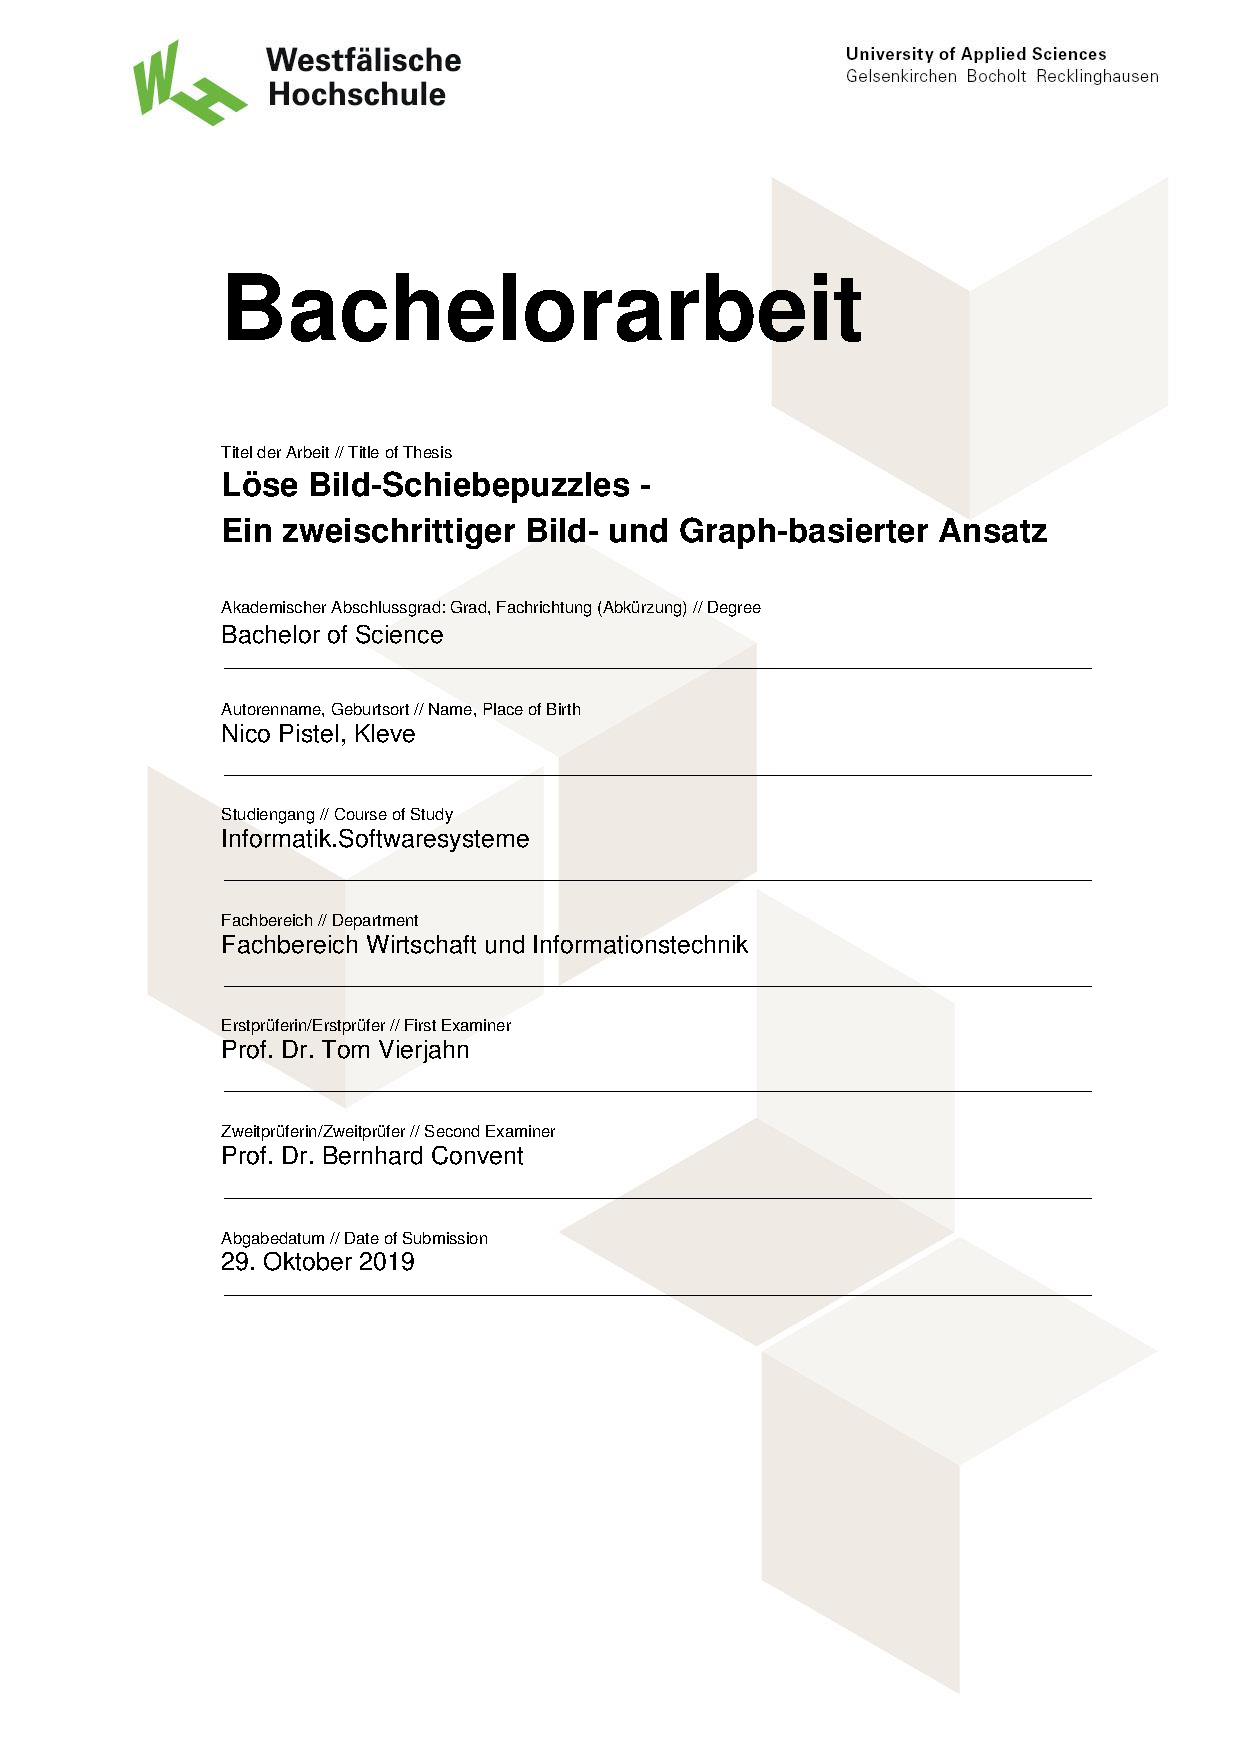
\includepdf[pages=-]{deckblatt.pdf}
\frontmatter

%\maketitle

\cleardoublepage
\chapter*{Abstract}
Schiebepuzzles - besonders das bekannte 15-Puzzle - stellen bereits seit Jahrzehnten eine Faszination für Puzzleliebhaber dar. Über die Jahre hat sich der Trend so entwickelt, dass die meisten Schiebepuzzle nicht mehr simple Zahlen oder Buchstaben abbilden, sondern ganze Bilder zerlegen. In dieser Arbeit werden zwei bekannte Probleme der Informatik untersucht und so kombiniert, dass diese einen möglichen Lösungsansatz zu dem bildbasierten Schiebepuzzle-Problem geben.

\tableofs
\lstlistoflistings
\listofalgorithms

\mainmatter

\chapter{Einleitung}
Schiebepuzzles wie das 15-Puzzle haben zum Ende des 19. Jahrhunderts das Interesse vieler amerikanischer Puzzle-Enthusiasten geweckt\cite{perelman,sloson} Heutzutage gibt es solche Schiebepuzzles in vielen Varianten. Dazu gehört die weitverbreitete Variante, bei der es nicht das Ziel ist, Zahlen aufsteigend zu sortieren, sondern bei dem das Puzzle aus einem Bild besteht, welches in quadratische Stücke aufgeteilt und durcheinander gemischt wurde. Das Originalbild lässt sich erst dann komplett erkennen, nachdem die Puzzlestücke in die richtige Reihenfolge gebracht wurden.
\begin{figure}[H]
    \centering
    \subfloat[15-Puzzle mit Zahlen (gemischt)\label{fig-15-puzzle-numbers-scrambled}]{
      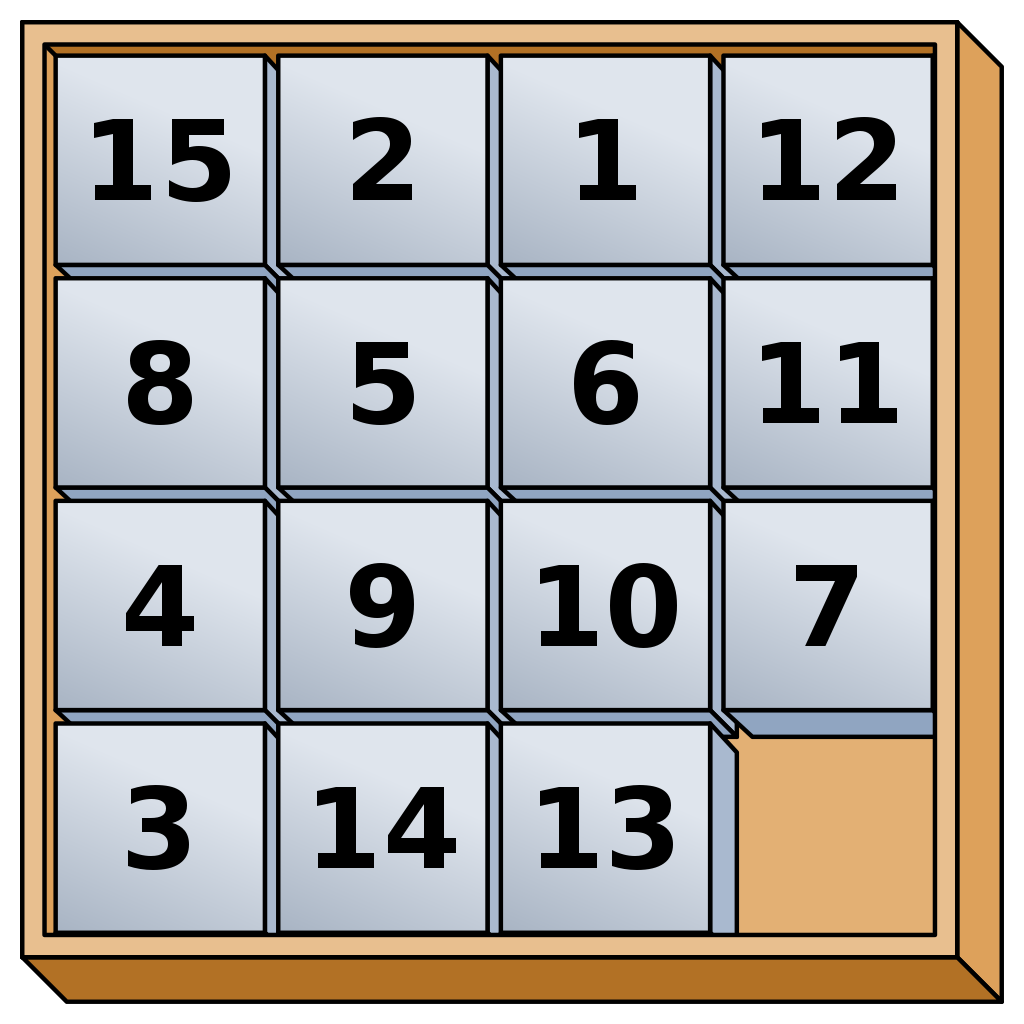
\includegraphics[width=0.25\linewidth]{img/15-puzzle-numbers-scrambled.png}
    }
    \quad\quad\quad\quad
    \subfloat[15-Puzzle mit Zahlen (gelöst)\label{fig-15-puzzle-numbers-solved}]{
      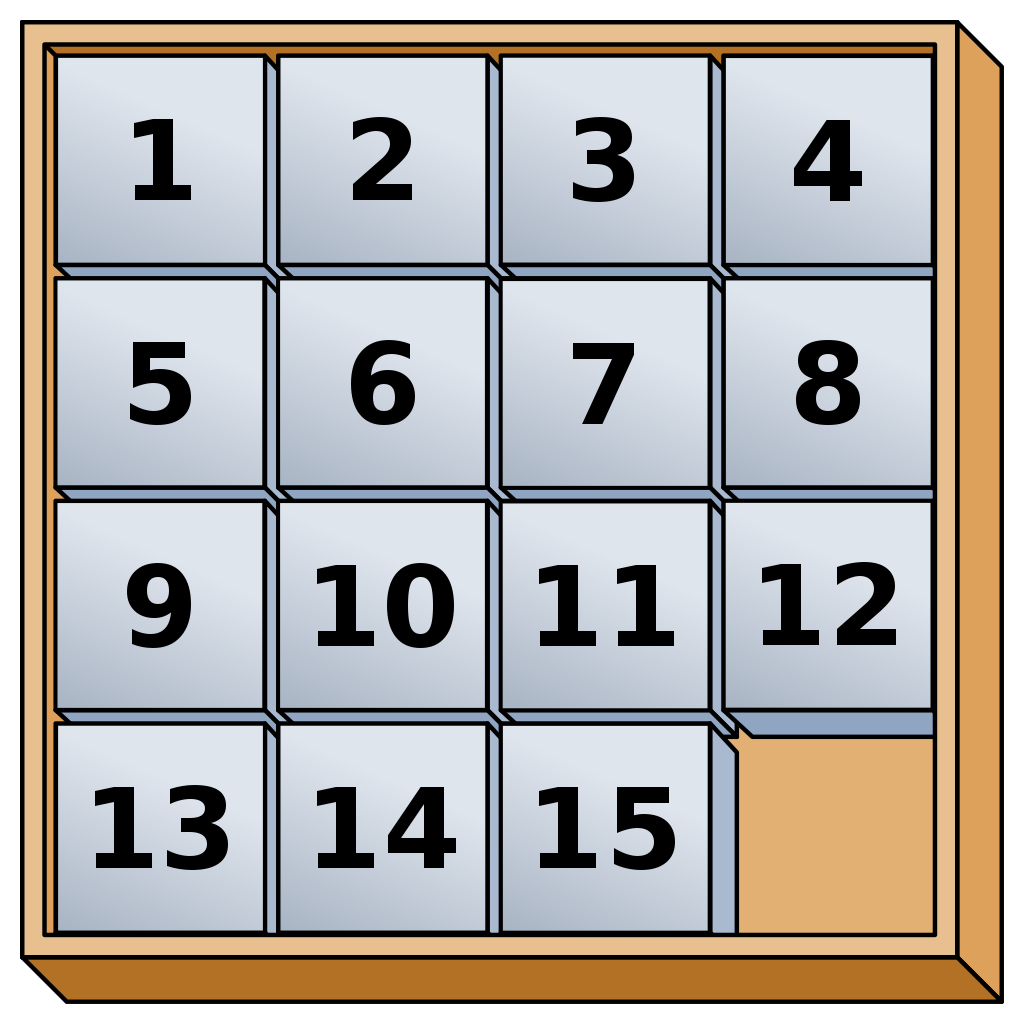
\includegraphics[width=0.25\linewidth]{img/15-puzzle-numbers-solved.png}
    }
    \\
    \subfloat[15-Puzzle mit Bild (gemischt)\label{fig-15-puzzle-image-scrambled}]{
        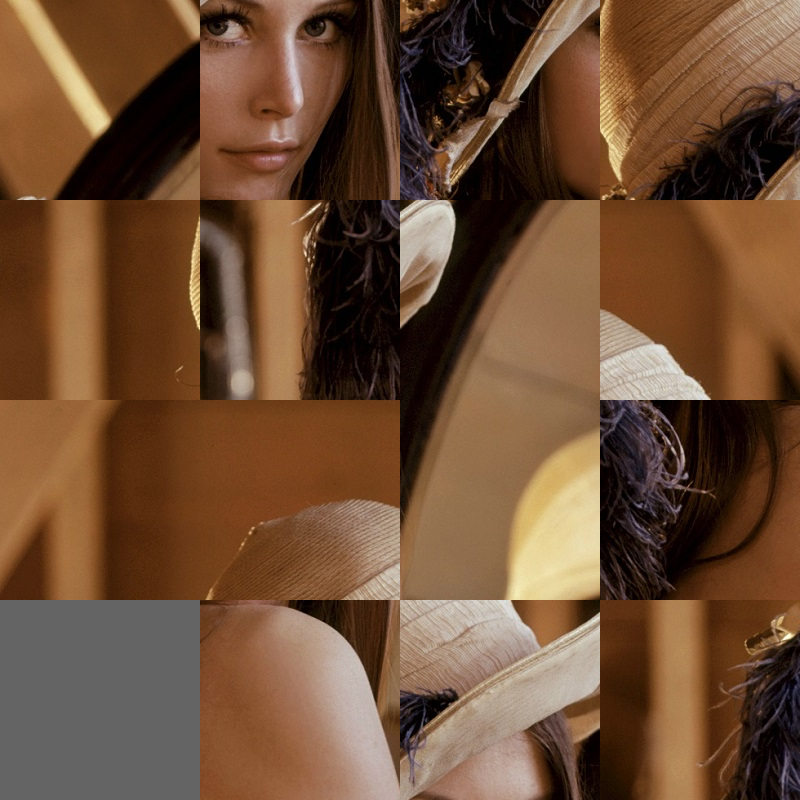
\includegraphics[width=0.25\linewidth]{img/fig-15-puzzle-image-scrambled.png}
    }
    \quad\quad\quad\quad
    \subfloat[15-Puzzle mit Bild (gelöst)\label{fig-15-puzzle-image-solved}]{
        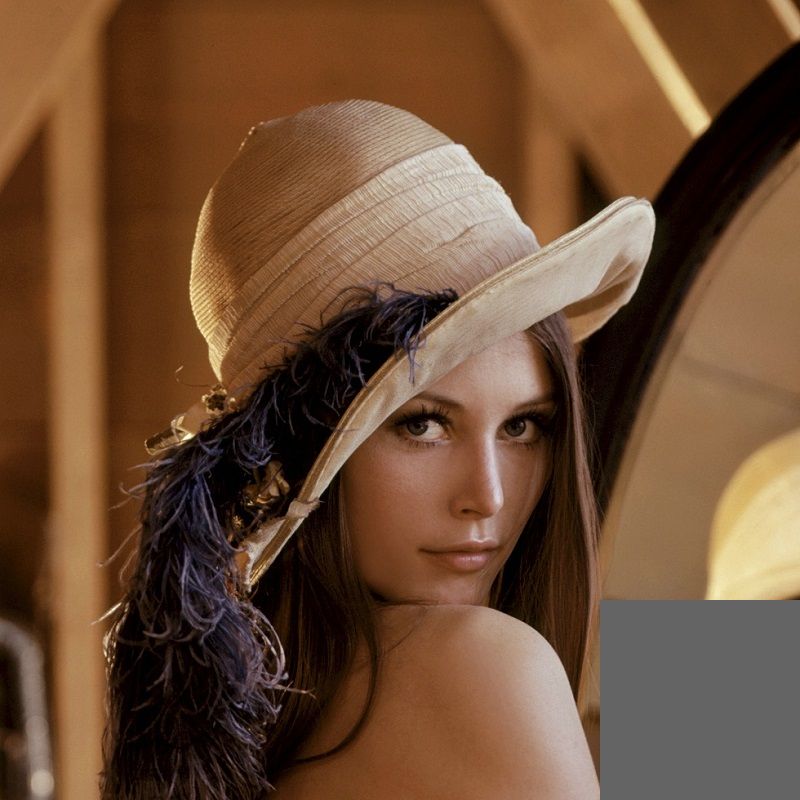
\includegraphics[width=0.25\linewidth]{img/fig-15-puzzle-image-solved.png}
    }
    \caption{Zwei Arten des 15-Puzzle}
    \label{fig-15-puzzle}
\end{figure}
In der Informatik ist das Lösen von Schiebepuzzles ein klassisches Problem der künstlichen Intelligenz und ein übliches Beispielproblem für die Modellierung und Illustration von Suchalgorithmen. Dabei beschränkt sich die meiste Literatur auf das Lösen des klassischen Schiebepuzzles mit Zahlen. Um diese Lösungsverfahren auf ein Schiebepuzzle mit Bild zu übertragen, muss also zuvor seperat das Originalbild rekonstruiert werden.

In dieser Arbeit wird genau solch ein zweischrittiger Ansatz erläutert und analyisert.
\section{Problemstellung und Zielsetzung}
In dieser Arbeit wird das Problem anhand des allgemeinen $N$-Puzzles betrachtet mit $N=m\times n-1$ (für das 15-Puzzle gilt somit $m=n=4$).
\marginpar{$m$: Anzahl der Zeilen}
\marginpar{$n$: Anzahl der Spalten}
Die $N$ Puzzlestücke sind dabei rechteckige Teile eines Bildes. Diese müssen nicht zwingend quadratisch sein, sollten aber alle das gleiche Seitenverhältnis aufweisen, damit diese als Teil eines Schiebepuzzles auch wirklich alle verschiebbar sind und sich somit in den Zustand eines Schiebepuzzles zusammensetzen lassen.

Die Position des leeren Feldes ist dabei nicht zwingend fest (so wie in \ref{fig-15-puzzle} z.\,B. immer unten-rechts) und kann variieren. Diese Position ist außerdem unbekannt und muss damit anhand der Zusammensetzung der restlichen $N$ Puzzleteilen und den bekannten Dimensionen des Puzzles ausgemacht werden.

Außerdem wird noch eine $m\times n$ Anordnung der $N$ Puzzlestücke (und dem leeren Feld) als Anfangszustand vorgegeben.

Folgende Fragen sollen dann (in dieser Reihenfolge) beantwortet werden:
\begin{enumerate}
    \item Wie sah das originale Bild aus und wo befindet sich das leere Feld im Ausgangsbild (wo fehlt also ein Stück des Bildes)?
    \item Ist das Puzzle lösbar, lässt sich also der gegebene Anfangszustand unter einer endlichen Sequenz von legalen Zügen (also ausschließlich durch das hin- und herschieben von Puzzlestücken) in den zuvor ermittelten Endzustand transformieren?
    \item Wie viele Schritte (Verschiebungen) sind mindestens nötig, um das Puzzle zu lösen und wie sieht ein optimaler Lösungsweg (ein Lösungsweg mit der kleinstmöglichen Anzahl an Verschiebungen) aus?
\end{enumerate}
Dazu wird ein vollautomatischer Schiebepuzzlelöser programmiert, der genau diese Schritte abarbeitet und am Ende bei einer gefundenen (optimalen) Lösung das Ergebnis dem Benutzer präsentiert.

Programmiert wird der Puzzlelöser in der Programmiersprache C++. Zur Analyse und Verarbeitung des Bildes wird die Open Source Computer Vision Bibliothek OpenCV verwendet.
\section{Aufbau der Arbeit}
Zunächst werden einige Grundlagen angesprochen, die den Umgang mit OpenCV erläutern und unter anderem aufklären, wie Bilder in OpenCV dargestellt und bearbeitet werden können.

Da zur Rekonstruktion Informationen wie die Kompatibilität (oder auch Ähnlichkeit) zweier Puzzlestücke notwendig ist, werden daraufhin einige Metriken vorgestellt, die diese Information repräsentieren.

Daraufhin wird die Rekonstruktion des Bildes weiter erläutert und ein Greedy Verfahren vorgestellt, welches dieses Problem mithilfe der zuvor berechneten Metriken löst.

Im nächsten Schritt wird das Puzzle mit seinem Anfangs- und Endzustand in ein äquivalentes Schiebepuzzle mit Zahlen übersetzt. Damit werden die nächsten Schritte anhand dem klassischen Zahlenpuzzle (jedoch weiterhin mit beliebigen Dimensionen und beliebigem Anfangs- und Endzustand) gezeigt.

Es wird dann erläutert, wie sich die Lösbarkeit eines Schiebepuzzles bestimmen lässt. Zusätzlich wird geklärt, wie sich zufällige Schiebepuzzle so generieren lassen, dass diese wahlweise immer lösbar oder immer unlösbar sind.

Zum Schluss werden Suchalgorithmen aus der künstlichen Intelligenz vorgestellt, die das eigentliche Lösen des Puzzles übernehmen. Dazu werden sowohl uninformierte Suchalgorithmen, als auch informierte Suchalgorithmen (welche Heuristiken in ihre Suche mit einbeziehen) untersucht und verglichen. An dieser Stelle werden somit auch verschiedene Heuristiken für Schiebepuzzle vorgestellt.
\chapter{OpenCV Grundlagen}
OpenCV (Open Source Computer Vision) ist eine Open Source Programmbibliothek, die mehr als 2500 optimierte Algorithmen aus den Bereichen Bildverarbeitung, maschinelles Sehen und maschinelles Lernen beinhaltet.\cite{opencv} OpenCV steht als freie Software (unter den Bedingungen der BSD-Lizenz) für die Programmiersprachen C++, Java, Python und MATLAB und den Betriebssystemen Windows, Linux, Android und Mac OS zur Verfügung. OpenCV wurde nativ in der Programmiersprache C++ geschrieben und bietet somit Schnittstellen an, die reibungslos mit der C++ Standard Template Library (STL) arbeiten.

OpenCV ist modular aufgebaut und bietet unter anderem folgende wichtige Module an:
\begin{itemize}
    \item \texttt{core} - Dieses Modul definiert einen Großteil der grundlegenden Funktionen und Datenstrukturen von OpenCV (wie z.\,B. die \texttt{cv::Mat}-Klasse beschrieben in \ref{section-mat}).
    \item \texttt{imgproc} - Das Image-Processing Modul implementiert Filter (sowohl lineare Filter als auch nicht lineare Filter), geometrische Bildtransformationen (lineare, linear-affine und perspektivische Transformationen), Histogramme und Methoden zur Konvertierung zwischen verschiedenen Farbräumen.
    \item \texttt{video} - Modul zur Videoanalyse, welches unter anderem Object-Tracking und auch Motion-Estimation Algorithmen implementiert.
    \item \texttt{calib3d} - Implementiert Algorithmen zur Kamerakalibrierung und Elemente zur 3D-Rekonstruktion.
    \item \texttt{features2d} - Bietet Algorithmen zum Erkennen und Matchen von Features in 2D an.
    \item \texttt{objdetect} - Erkennung von Objekten vordefinierter Klassen (z.\,B. Gesichtserkennung)
    \item \texttt{highgui} - Bietet dem Programmierer Möglichkeiten an, simple grafische Benutzungsschnittstellen zu erstellen.
\end{itemize}
\section{Mat - Der OpenCV Bild-Container}\label{section-mat}
Die OpenCV Programmbibliothek war ursprünglich eine Programmbibliothek für die Programmiersprache C. Damit wurden die Datenstrukturen der Bibliothek als C-Structs implementiert, wodurch der Programmierer selber sicherstellen musste, dass der Speicher für diese Datenstrukturen richtig allokiert, deallokiert und gegebenenfalls auch kopiert wird.

Mit der Version OpenCV 2.0 wurde erstmals eine neue C++ Schnittstelle implementiert. Auf Basis der objektorientierten Prinzipien von C++ wie z.\,B. Klassen, Konstruktoren (auch Copy- und Move-Konstruktoren), Destruktor, Resource Acquisition Is Initialization (RAII), Operatorüberladung und Template-Programmierung, somit entstand ein abstrakteres und damit auch einfacheres Interface für den Umgang mit Bildern in OpenCV. Die Klasse \texttt{cv::Mat} ist ein wichtiger Bestandteil dieser Schnittstelle.

Die \texttt{cv::Mat} Klasse stellt eine $n$-dimensionale \textit{dense} Matrix da. Im Gegensatz zu einer \textit{sparse} Matrix (im OpenCV durch die Klasse \texttt{cv::SparseMat} implementiert), welche nur Elemente $\neq0$ speichert, werden bei \texttt{cv::Mat} alle Elemente gespeichert. Die Elemente können sowohl Single-Channel bzw. skalar (z.\,B. Intensität bei Graustufenbildern) oder Multi-Channel bzw. vektorwertig (z.\,B. Intensität einzelner Farbchannel) sein.

Bei $n$-Dimensionen und Dimensionsgrößen $(m_1,\dots,m_n)$ ergeben sich somit $$N=\prod_{k=1}^{n}m_k$$ Elemente, welche intern kontinuierlich in einem $N$-Element großen (eindimensionalem) Array gespeichert sind. Der (nullbasierte) Array-Index $j$ eines Elementes mit den Dimensions-Indizes $(i_1,\dots,i_n)$ lässt sich dann durch folgende rekursive Relation berechnen\cite{opencv2} (mit $j=j_n$): $$j_k=\begin{cases}j_{k-1}\cdot m_k+i_k,&k\neq0\\0&k=0\end{cases}$$.

Im zweidimensionalen Fall ($n=2$) reduziert sich dies zu $j=i_1\cdot m_2+i_2$. Mit $i_1$ als Zeilenindex, $i_2$ als Spaltenindex und der Anzahl an Spalten $m_2$. Somit werden zweidimensionale Matrizen also Zeile-für-Zeile gespeichert, dreidimensionale Matrizen zunächst Ebene-für-Ebene und dann jede Ebene wieder Zeile-für-Zeile.

Dieses Speicherlayout ist üblich für \textit{dense} Arrays und ist kompatibel mit anderen Bibliotheken, die ein solches Speicherlayout voraussetzen. Dazu gehört auch die C++ STL. Diese Kompatibilität ermöglicht es nicht nur, STL-Algorithmen auf die Daten eines \texttt{cv::Mat}-Objektes anzuwenden, sondern es bietet sich auch die Möglichkeit an, selbst allokierte Daten in ein \texttt{cv::Mat}-Objekt zu wrappen und diese Daten dann mit OpenCV spezifischen Methoden zu bearbeiten.

Die \texttt{cv::Mat}-Klasse ist stark an die Matrizen aus MATLAB angelehnt, womit OpenCV die Möglichkeit bietet Matrizen im MATLAB-Style zu initialisieren mit z.\,B. \texttt{cv::Mat::zeros()} um alle Elemente der Matrix mit $0$ zu initialisieren, \texttt{cv::Mat::ones()} um alle Elemente mit $1$ zu initialisieren und \texttt{cv::Mat::eye()} zur Konstruktion einer Einheitsmatrix.

Die Datenstrukturen von OpenCV (und damit auch \texttt{cv::Mat}) implementieren bereits die nötigen Maßnahmen zur Speicherverwaltung, womit dies nicht vom Programmierer übernommen werden muss. Dabei sei jedoch zu beachten, dass \texttt{cv::Mat} jedoch nicht wie die meisten C++ Datenstrukturen mit dynamischem Speicher (z.\,B. \texttt{std::vector}) implementiert ist.

Ein \texttt{std::vector} wird beim Kopieren (entweder beim Initialisieren eines anderen Vectors mit dem Kopier-Konstruktor oder durch den Assignment-Operator) komplett kopiert und bekommt seinen eigenen Speicher, der nun die gleichen Daten enthält wie der Originalvector. Es wird kein Speicher zwischen den beiden Objekten geteilt und jedes Objekt ist für seinen eigenen Speicher zuständig. Um die lineare Laufzeit beim Kopieren zu umgehen, wo diese nicht nötig ist, wird Referenzübergabe verwendet. Auch das Kopieren von temporären Objekten, sogenannten rvalues (da solche Objekte bei nur links vom Assignment-Operator stehen dürfen), lässt sich seit C++11 mithilfe von Move-Semantiken in konstanter Zeit durchführen.

Im Gegensatz dazu teilen \texttt{cv::Mat}-Objekte ihre Resourcen (den darunterliegenden Speicher) gegebenenfalls mit anderen \texttt{cv::Mat}-Objekten. Dazu implementiert \texttt{cv::Mat} Reference-Counting und arbeitet somit ähnlich wie der Smart-Pointer \texttt{std::shared\_ptr} der C++11-Library oder auch wie Objekte in anderen Programmiersprachen wie Java oder C\#. Dies hat zu Folge, dass die Destruktoren von \texttt{cv::Mat}-Objekten zunächst die Reference-Count dektrementieren und den Speicher erst dann wieder freigeben, wenn die Reference-Count mit dem destrukten des letzten Objektes auf $0$ gefallen ist. Der Vorteil hierbei ist, dass das Kopieren einer Matrix genau genommen die Daten nicht wirklich kopiert, sondern lediglich den Matrix-Header (mit Metadaten wie Dimensionsgrößen und der Adresse zum Speicher der Daten) übernimmt und den Reference-Counter inkrementiert. Das Kopieren einer Matrix ist also unabhängig von der Größe der Matrix und somit konstant. Um eine Matrix vollständig zu kopieren bietet OpenCV in der \texttt{cv::Mat}-Klasse die Methode \texttt{cv::Mat::clone()} an.

Die Kopiersemantik von \texttt{cv::Mat} ist dann von wichtiger Bedeutung, wenn es gilt, einen Teilbereich einer Matrix zu extrahieren oder zu ändern. Solche Bereiche werden als Region of Interest (ROI) bezeichnet und können eine oder mehrere Zeilen, eine oder mehrere Spalten, eine Diagonale oder ein rechteckiger Bereich aus der Matrix sein. Diese Operationen sind weiterhin alle $\Theta(1)$, da lediglich ein neuer Matrix-Header erstellt werden muss und die eigentlichen Elemente der Matrix nicht kopiert werden, sondern nur referenziert werden. Damit wirken sich Änderungen der Daten in einer Matrix also auch implizit auf alle anderen Matrizen aus, die diese Daten referenzieren.

\section{Saturate-Casting}\label{section-sat}
Die einzelnen Pixels eines Bildes sind in OpenCV Elemente einer zweidimensionalen \texttt{cv::Mat}. Ob diese Elemente skalar oder vektorwertig sind hängt vom gewählten Farbraum ab. Die Wertebereiche der einzelnen Channel eines Elementes hängen wiederum vom gewählten Datentyp ab (vgl. \ref{section-pixeltypes}). Dabei werden oftmals 8- oder 16-bit (signed oder unsigned) per Channel gewählt. Für unsigned 8-bit (Datentyp \texttt{cv::uchar} in OpenCV) stehen damit nur ganzzahlige Werte aus dem (halboffenen) Intervall $[0, 256)$ zu Verfügung. Viele Operationen auf Bildern (z.\,B. das Interpolieren von Bildern oder das Konvertieren zwischen verschiedenen Farbräumen) können Werte ausserhalb dieses Intervalles erzeugen. Anstatt jedoch nur die niedrigsten 8 Bits des Ergebnisses zu verwenden (was in einem Bild unmittelbar zu sichtbaren Artifakten führt), bietet OpenCV einen \texttt{cv::saturate\_cast<>()} an, welcher den berechneten Wert auf den nächsten Wert im zugelassenen Wertebereich vom Datentyp abbildet. Dazu wird der Wert zunächst gerundet. Falls der gerundet Wert ausserhalb des gültigen Wertebereiches liegt, wird dieser auf den nächsten Wert gültigen Wert gesetzt (jeweils auf das Minimum oder Maximum der Intervalls, je nachdem ob der Wert auf dem Zahlenstrahl links oder rechts vom Intervall liegt). Der letzte Schritt wird auch als \textit{Clamping} bezeichnet. Eine mögliche Implementation\cite{opencv3} für einen 8-bit Channel mit einem berechneten Wert $v$ ist $$v'=\min\{\max\{\lfloor v+0.5\rfloor,0\},255\}$$.
\section{Datentypen für Pixel}\label{section-pixeltypes}
Anstatt die Wahl des Datentyps für Pixel generisch zu halten (mithilfe von C++ Templates), gibt OpenCV eine feste limitierte Menge an primitiven Datentypen für Matrizen vor.\cite{opencv3} Der Grund dafür ist, dass große Template Klassen die Compilezeit und die größe des Codes stark erhöhen. Außerdem lassen sich Templates nur schlecht in Definition und Implementation aufteilen (wie es sonst mit Header- und Source-Dateien üblich ist). Des Weiteren besitzen die anderen Sprachen, welche von OpenCV unterstützt werden (Python, MATLAB und Java), keine oder nur begrenzte Sprachkonstrukte, welche die Implementation von Templates ermöglichen würde. Stattdessen basiert die aktuelle OpenCV Implementation hauptsächlich auf Polymorphismus. In C++ stehen aus Performancegründen (um die dynamische Laufzeitbindung von polymorphen Methoden zu vermeiden) jedoch einzelne Template Klassen, Methoden und Funktionen zur Verfügung (dazu gehört auch der \texttt{cv::saturate\_cast<>()}.

In OpenCV stehen folgende primitive skalare Datentypen für Matrizen zur Verfügung:
\begin{itemize}
    \item 8-bit unsigned Integer - \texttt{cv::uchar}
    \item 8-bit signed Integer - \texttt{cv::schar}
    \item 16-bit unsigned Integer - \texttt{cv::ushort}
    \item 16-bit signed Integer - \texttt{cv::short}
    \item 32-bit signed Integer - \texttt{cv::int}
    \item 32-bit floating-point Zahl - \texttt{cv::float}
    \item 64-bit floating-point Zahl - \texttt{cv::double}
\end{itemize}
Für Multi-Channel Matrizen wird vorausgesetzt, dass jeder Channel den gleichen Datentyp besitzt (außerdem muss dieser natürlich einer der oben aufgeführten Datentypen sein). Des Weiteren ist die maximale Anzahl an möglichen Channels per Matrixelement auf $512$ begrenzt.

Die oben aufgeführten Typen werden zwar als Template-Argument für einzelne Funktionen von OpenCV verwendet (z.\,B. für den bereits erwähnten \texttt{cv::saturate\_cast<>()}), spezifizieren aber nicht den Datentyp für Matrixelemente (da \texttt{cv::Mat} schließlich nicht generisch ist). Stattdessen besitzen diese Klassen dann einen weiteren Parameter im Konstruktur, mit dem der Datentyp angegeben werden kann. Für die skalaren Typen gilt dabei folgende Enumeration:
\begin{lstlisting}[numbers=none,frame=none]
enum {
    CV_8U  = 0,
    CV_8S  = 1,
    CV_16U = 2,
    CV_16S = 3,
    CV_32S = 4,
    CV_32F = 5,
    CV_64F = 6
};
\end{lstlisting}
Die Namen für Multi-Channel Konstanten mit $k=1\dots4$ Channels entsprechen dem Namen des Datentyps eines Channels (entsprechend der obigen Enumeration), gefolgt von einem \texttt{C}$k$. Ein Drei-Channel Array vom Typen 16-bit unsigned Integer entspricht also der Konstanten \texttt{CV\_16UC3}.

Um einen Matrix mit mehr als vier Channels zu initialisieren oder falls die Anzahl der Channel bei der Compilezeit unbekannt ist, lassen sich die Makros \texttt{CV\_U8C(n)} bis \texttt{CV\_64FC(n)} verwenden. Genau genommen generieren diese Makros lediglich eine numerische Konstante, die intern eine Kombination von Datentyp und Anzahl an Channels identifiziert. Dazu wird die Konstante des Datentyps (entsprechend den Werten in der Enumeration) in die niedrigsten 3 Bits gehschrieben und die Anzahl der Channel dekrementiert (da $0$ Channel sowieso nicht zugelassen sind, lässt sich dadurch eine Möglichkeit mehr darstellen) und in die restlichen Bits geschrieben. Dementsprechend sind für die Anzahl der Channels standardmäßig $\log_2(512)=9$ Bits vorgesehen. Die Berechnung der numerischen Konstante eines Multi-Channel Datentyps ist in OpenCV mit dem Makro \texttt{CV\_MAKETYPE(depth, cn)} implementiert, dabei entspricht \texttt{depth} der numerischen Konstante des Datentyps entsprechend der Enumeration und \texttt{cn} die Anzahl der Channel (\texttt{cn > 0}). Eine mögliche Implementation nach \cite{opencv4} dieses Makros sieht folgendermaßen aus:
\begin{lstlisting}[numbers=none,frame=none]
#define CV_MAKETYPE(depth, cn) (((depth) & 7) | (((cn)-1) << 3))
\end{lstlisting}
Damit ergeben sich viele equivalente Möglichkeiten, den Datentyp einer Matrix festzulegen. So gilt z.\,B. \texttt{2 == CV\_16U == CV\_16UC1 == CV\_16UC(1) == CV\_MAKETYPE(CV\_16U, 1) == (2 \& 7) | ((1 - 1) << 3) == 2}, was mit der ursprünglichen Definition aus der Enumeration übereinstimmt.

Was genau die Werte eines einzelnen Elementes darstellen, hängt vom Farbraum des Bildes ab. Beim Einlesen eines Bildes in OpenCV mit der Funktion \texttt{cv::imread()} lässt sich als Parameter mit angeben, ob dieses Bild als Graustufenbild gelesen werden soll (\texttt{IMREAD\_GRAYSCALE}) oder als Farbbild (\texttt{IMREAD\_COLOR}). Als Rückgabewert liefert die Funktion eine (zweidimensionale) Matrix in den Dimensionen des ursprünglichen Bildes. Jedes Element der Matrix stellt einen Bildpunkt des Bildes in dem entsprechenden Farbraum (wird dieser nicht explizit angegeben, so wird implizit der Parameter \texttt{IMREAD\_COLOR} verwendet) dar. Bei Graustufenbildern bestehen diese Elemente nur aus einem Channel (der Intensität dieses Bildpunktes), während bei Farbbildern das BGR-Format verwendet wird. Hierbei steht der Wert jedes Channels (von insgesamt drei) für die Intensität der entsprechenden Farbe (\textbf{B}lau, \textbf{G}rün oder \textbf{R}ot) im Bildpunkt. Das BGR-Format ist abgesehen von der Reihenfolge der Farbchannel identisch zu dem bekannten RGB-Format.

Um Bilder zwischen verschiedenen Farbräumen zu konvertieren lässt sich die OpenCV Funktion \texttt{cv::cvtColor()} verwenden. Es lässt sich als Parameter angeben, welche Art von Konvertieren stattfinden soll (z.\,B. \texttt{COLOR\_BGR2GRAY}).\cite{opencv5}

\section{Beispiel: Verwendung von Matrizen und Region of Interests}
Es folgt ein Codeausschnitt, der die Eigenschaften von \texttt{Mat} nach Abschnitt \ref{section-mat} nochmals aufzeigt.
\begin{lstlisting}[caption=Verwendung von Mat und ROI, label=lst-mat-example]
cv::Mat a(256, 256, CV_8UC3, cv::Scalar(100, 100, 100));
cv::Mat b = a;
cv::Mat c = a.clone();

a.colRange(50, 80).setTo(cv::Scalar(255, 0, 0));
b.diag().setTo(cv::Scalar(0, 255, 0));
c({ 0, 20 }, { 0, 20 }).setTo(cv::Scalar(0, 0, 255));

cv::namedWindow("a");
cv::imshow("a", a);

cv::namedWindow("b");
cv::imshow("b", b);

cv::namedWindow("c");
cv::imshow("c", c);

cv::waitKey();
cv::destroyAllWindows();
\end{lstlisting}
Im Beispiel wird zunächst eine zweidimensionale $256\times256$ Matrix \texttt{a} vom Typen \texttt{CV\_8UC3} angelegt und jeder der drei 8-bit Farbchannel mit $100$ initialisiert, was im BGR Farbraum einem Grauton entspricht. Die Matrix benötigt somit insgesamt exakt $192$ Kibibyte, um die Farbwerte der Pixel zu speichern (mit Headerdaten ist diese natürlich noch größer). Die Initialisierung von \texttt{b} in der darauffolgenden Zeile führt wie in \ref{section-mat} beschrieben lediglich dazu, dass die Headerdaten von \texttt{a} übernommen werden. Damit befindet sich weiterhin nur ein (komplett graues) Bild im Speicher, welches jedoch von zwei verschiedenen \texttt{Mat}-Objekten (\texttt{a} und \texttt{b}) referenziert wird. Die Initialisierung von Matrix \texttt{c} entspricht hingegen einer tiefen Kopie der Matrix \texttt{a}, wodurch nun zwei (gleiche) Bilder im Speicher liegen. Diese Operation muss den kompletten Speicher von \texttt{a} kopieren, was zu einem linearen Laufzeitverhalten fürt.

Die nächsten Zeilen zeigen, wie ROIs in OpenCV verwendet werden können, um Teilbereiche einer Matrix zu extrahieren und zu bearbeiten. Zeile 5 erstellt eine temporäre Matrix, welche auf den gleichen Speicherbereich von \texttt{a} zeigt, die Headerdaten jedoch so definiert werden, dass diese Matrix nur einen Teilbereich von \texttt{a} schreiben und lesen kann. Als ROI werden hier die Spaltenvektoren von \texttt{a} mit Spaltenindizes (nullbasiert) aus dem Intervall $[50,80)$ genommen. Damit ergibt sich eine temporäre $256\times30$ Matrix. Alle Elemente dieser Matrix werden daraufhin blau gefärbt, wodurch natürlich auch die entsprechenden Spalten in \texttt{a} betroffen sind und damit auch implizit das Bild der Matrix \texttt{b} verändert wird (was schließlich das Bild aus der Matrix \texttt{a} ist). Zeile 6 färbt die Hauptdiagonale von \texttt{b} $\{b_{ij}:(i,j)\in[0,256)^2\land i=j\}$ grün (was wiederum die Matrix \texttt{a} mit betrifft). Die Matrix \texttt{c} hat zu diesem Zeitpunkt immer noch ein rein graues Bild. Zeile 7 zeigt, wie man eine beliebige rechteckige ROI aus einer Matrix extrahiert. Im Beispiel wird eine $20\times20$ ROI erstellt mit den Matrixelementen $\{c_{ij}:0\leq i,j<20\}$, welche daraufhin rot gefärbt werden. Diese Operation betrifft ausschließlich die Matrix \texttt{c}; \texttt{a} und \texttt{b} werden nicht verändert.

Die nächsten Zeilen stellen den Inhalt der Matrizen dar. Die Ausgabe ist in \ref{fig-opencv-mat} dargestellt. Wie erwartet zeigen die Matrizen \texttt{a} und \texttt{b} das selbe Bild.
\begin{figure}[H]
    \centering
    \subfloat[\label{fig-opencv-mat-a}]{
      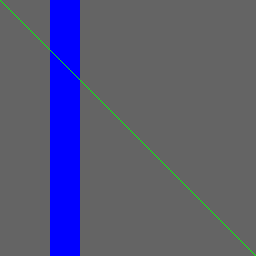
\includegraphics[width=0.25\linewidth]{img/a.png}
    }
    \quad\quad
    \subfloat[\label{fig-opencv-mat-b}]{
      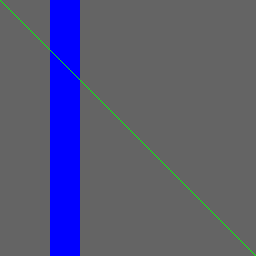
\includegraphics[width=0.25\linewidth]{img/b.png}
    }
    \quad\quad
    \subfloat[\label{fig-opencv-mat-c}]{
      
\includegraphics[width=0.25\linewidth]{img/c.png}
    }
    \caption{Ausgabe vom Mat und ROI Beispiel}
    \label{fig-opencv-mat}
\end{figure}
\section{Transformation von Bildern}
Um bekannte lineare Transformationen (Skalierung, Rotation, Scherung) und affine Transformationen (lineare Transformationen mit einer Translationskomponente) auf Bildern anzuwenden, bietet OpenCV die Funktion \texttt{cv::warpAffine()} an. Neben dem Ausgangsbild, auf welches die Transformation angewendet werden soll, und einem Zielbild, welches das Ergebnis der Transformation halten soll, übernimmt diese Funktion noch eine $2\times3$ Transformationsmatrix.

Eine affine Transformation $T:\mathbb{R}^2\rightarrow\mathbb{R}^2$ bildet einen Vektor $\vec{x}=\begin{bmatrix}x\\y\end{bmatrix}\in\mathbb{R}^2$ auf einen Vektor $T(\vec{x})\in\mathbb{R}^2$ ab. Eine solche Transformation hat die Form
\begin{gather*}
    T(\vec{x})=\mathbf{A}\vec{x}+\vec{b}
\end{gather*}
mit $\mathbf{A}=\begin{bmatrix}a_{11}&a_{12}\\a_{21}&a_{22}\end{bmatrix}\in\mathbb{R}^{2\times2}$ und dem Translationsvektor $\vec{b}\in\mathbb{R}^2$.

Für $\vec{b}=\vec{0}$ ist $T$ eine lineare Transformation. Eine solche Transformation erfüllt folgende Bedingung ($T$ ist homogen und additiv): $T(\alpha\vec{u}+\vec{v})=\alpha T(\vec{u})+T(\vec{v})$ für ein Skalar $\alpha\in\mathbb{R}$ und zwei Vektoren $\vec{u},\vec{v}\in\mathbb{R}^2$. Eine Implikation dieser Bedingung ist, dass der Nullvektor stets auf sich selber abgebildet wird: $T(\vec{0})=T(0\cdot\vec{e}_1+0\cdot\vec{e}_2)=0\cdot T(\vec{e}_1)+0\cdot T(\vec{e}_2)=\vec{0}+\vec{0}=\vec{0}$.

Wird $\vec{x}$ in homogenen Koordinaten betrachtet ($\vec{x}=\begin{bmatrix}x&y&1\end{bmatrix}^\mathsf{T}$), so lässt sich eine Matrix $\mathbf{M}$ zur Transformation $T$ angeben.
\begin{align*}
    T(\vec{x})&=\mathbf{A}\vec{x}+\vec{b}\\
    T(\vec{x})&=\begin{bmatrix}a_{11}&a_{12}\\a_{21}&a_{22}\end{bmatrix}\cdot\begin{bmatrix}x\\y\end{bmatrix}+\begin{bmatrix}b_1\\b_2\end{bmatrix}\\
    T(\vec{x})&=x\cdot\begin{bmatrix}a_{11}\\a_{21}\end{bmatrix}+y\cdot\begin{bmatrix}a_{12}\\a_{22}\end{bmatrix}+1\cdot\begin{bmatrix}b_1\\b_2\end{bmatrix}\\
    T(\vec{x})&=\underbrace{\begin{bmatrix}a_{11}&a_{12}&b_1\\a_{21}&a_{22}&b_2\end{bmatrix}}_{\eqqcolon\mathbf{M}\in\mathbb{R}^{2\times3}}\cdot\begin{bmatrix}x\\y\\1\end{bmatrix}
\end{align*}
Die Funktion \texttt{cv::warpAffine()} transformiert das Originalbild dann so, dass $$dst(\vec{x})=src(T^{-1}(\vec{x}))$$.\cite{opencv6}

Damit arbeitet die Funktion also mit der inversen Transformation, welche sich mit der Funktion \texttt{cv::invertAffineTransform()} berechnen lässt. Standardmäßig wird dies bereits von \texttt{cv::warpAffine()} übernommen. Liegt die Transformation jedoch schon invertiert vor, lässt sich diese auch an die Funktion übergeben. Das Setzen von dem \texttt{WARP\_INVERSE\_MAP}-Flag bewirkt dann, dass das Invertieren der Transformation übersprungen wird.

Um Beispielsweise das Bild um 90° (gegen den Uhrzeigersinn) um den Bildmittelpunkt zu rotieren, lässt sich eine Transformation als Komposition von Translation und Rotation angeben. Dabei ist zu beachten, dass der Ursprung des Koordinatensystems sich an der linkeren oberen Ecke des Bildes befindet. Die x-Achse zeigt nach rechts und die y-Achse nach unten. Bei einem Bild mit Breite $w$ und Höhe $h$ gilt $(x,y)\in[0,w)\times[0,h)$ womit sich der Bildmittelpunkt bei $(\frac{w-1}{2},\frac{h-1}{2})$ befindet.

Die entsprechende Transformationsmatrix $\mathbf{M}$ lautet dann $$\mathbf{M}=\begin{bmatrix}1&0&\frac{w-1}{2}\\0&1&\frac{h-1}{2}\end{bmatrix}\cdot\underbrace{\begin{bmatrix}0&1&0\\-1&0&0\\0&0&1\end{bmatrix}}_{Rotation}\cdot\begin{bmatrix}1&0&-\frac{w-1}{2}\\0&1&-\frac{h-1}{2}\\0&0&1\end{bmatrix}$$.

Die homogene Komponente wird bis zur letzten Transformation erhalten, um die Komposition von affinen und linearen Transformationen zu ermöglichen. Da \texttt{cv::warpAffine()} jedoch eine $2\times3$ Matrix benötigt, wird die letzte Matrix auch als $2\times3$ Matrix angegeben.
\begin{figure}[H]
    \centering
    \subfloat[src\label{fig-opencv-affine-1-src}]{
      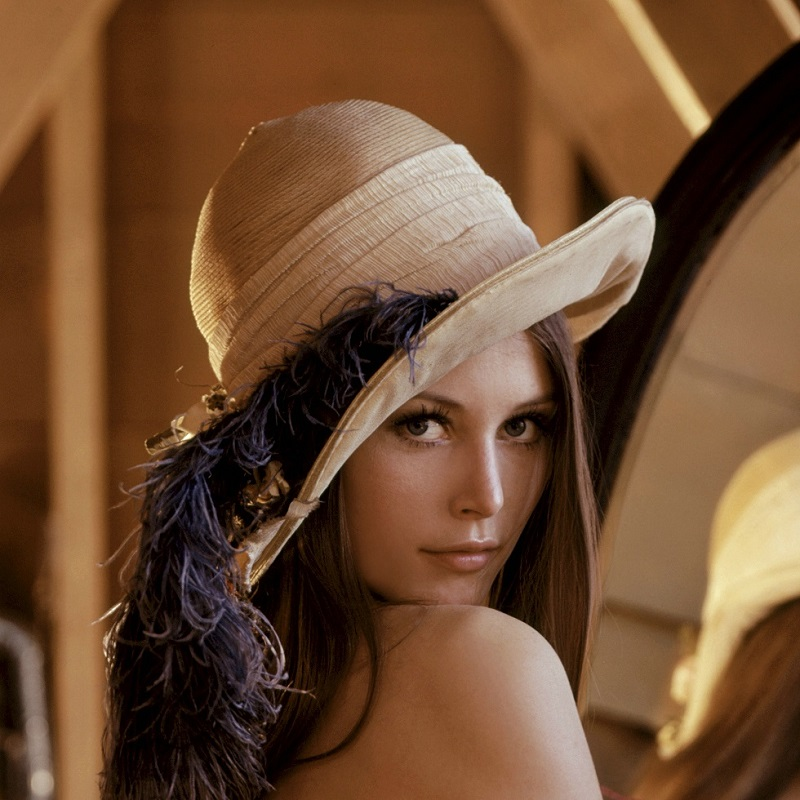
\includegraphics[width=0.25\linewidth]{img/affine_1_src.png}
    }
    \quad\quad\quad\quad
    \subfloat[dst\label{fig-opencv-affine-1-dst}]{
      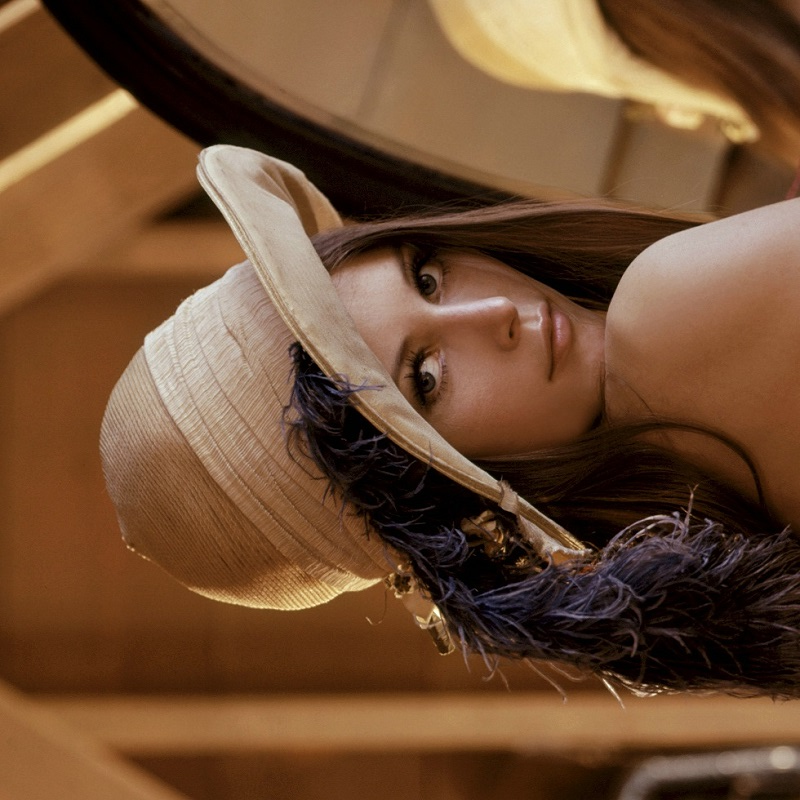
\includegraphics[width=0.25\linewidth]{img/affine_1_dst.png}
    }
    \caption{Rotation als affine Transformation}
    \label{fig-opencv-affine-1}
\end{figure}
Um die entsprechende Transformationsmatrix einer beliebigen Rotation direkt zu bekommen, bietet OpenCV die Funktion \texttt{cv::getRotationMatrix2D()} an, welche neben dem Rotationswinkel (gemessen in Grad und gegen dem Uhrzeigersinn) auch einen Punkt übernimmt, um den rotiert werden soll.

Da eine affine Transformation Dreiecke auf Dreiecke abbildet, lässt sich eine eindeutige affine Transformation finden, welche eine geordnete Menge von drei nicht-kollinearen Punkten auf eine andere Menge dieser Art abbildet.

OpenCV bietet dafür die Funktion \texttt{cv::getAffineTransform()} an. Diese übernimmt drei Punkte $(x_i,y_i)$, welche auf drei andere Punkte $(x_i^\prime,y_i^\prime)$ abgebildet werden sollen ($1\leq i\leq3$). Als Ergebnis liefert diese Funktion eine $2\times3$ Transformationsmatrix $\mathbf{M}$. Dabei ist $\mathbf{M}$ genau die Matrix der affinen Transformation, für die 
\begin{align}
\begin{bmatrix}x_i^\prime\\y_i^\prime\end{bmatrix}=\mathbf{M}\cdot\begin{bmatrix}x_i\\y_i\\1\end{bmatrix},1\leq i\leq3 \label{eq1}
\end{align}.\cite{opencv6}

Mit $$\mathbf{M}=\begin{bmatrix}m_{11}&m_{12}&m_{13}\\m_{21}&m_{22}&m_{23}\end{bmatrix}$$ wird dann intern von der Funktion ein $6\times6$ Gleichungssystem gelöst, um die Koeffizienten von $\mathbf{M}$ herauszufinden. Das Gleichungssystem lautet $$\begin{bmatrix}x_1&y_1&1&0&0&0\\x_2&y_2&1&0&0&0\\x_3&y_3&1&0&0&0\\0&0&0&x_1&y_1&1\\0&0&0&x_2&y_2&1\\0&0&0&x_3&y_3&1\end{bmatrix}\cdot\begin{bmatrix}m_{11}\\m_{12}\\m_{13}\\m_{21}\\m_{22}\\m_{23}\\\end{bmatrix}=\begin{bmatrix}x_1^\prime\\x_2^\prime\\x_3^\prime\\y_1^\prime\\y_2^\prime\\y_3^\prime\\\end{bmatrix}$$.

Alternativ dazu lassen sich auch zwei Matrizen $\mathbf{A},\mathbf{B}$ definieren mit $$\mathbf{A}=\begin{bmatrix}x_1&x_2&x_3\\y_1&y_2&y_3\\1&1&1\end{bmatrix},\mathbf{B}=\begin{bmatrix}x_1^\prime&x_2^\prime&x_3^\prime\\y_1^\prime&y_2^\prime&y_3^\prime\end{bmatrix}$$.

Die Matrix $\mathbf{A}$ bildet die drei Standardbasisvektoren des $\mathbb{R}^3$ ($\vec{e}_1,\vec{e}_2,\vec{e}_3$) auf die drei Vertices des Dreiecks ab (in homogenen Koordinaten). Es gilt also $\begin{bmatrix}x_i&y_i&1\end{bmatrix}^\mathsf{T}=\mathbf{A}\vec{e}_i,1\leq i\leq3$. Allgemein werden alle Vektoren $\begin{bmatrix}\alpha&\beta&\gamma\end{bmatrix}^\mathsf{T}$ mit $\alpha+\beta+\gamma=1$ auf einen Vektor in der Ebene des Dreiecks (also einen Vektor mit $1$ als homogene Komponente) abgebildet. Gilt außerdem noch $\alpha,\beta,\gamma\geq0$, dann ist dies sogar ein Vektor im Dreieck.

Die Matrix $\mathbf{B}$ hat ähnliche Eigenschaften wie $\mathbf{A}$. Hier wurden lediglich die Vertices des zweiten Dreiecks als Spaltenvektoren der Matrix verwendet. Außerdem fehlt hier jeweils die homogene Komponente in den Spaltenvektoren. Dadurch ist der Ergebnisvektor direkt ein Vektor im $\mathbb{R}^2$ (ohne homogene Komponente).

Damit lässt sich $\mathbf{M}$ nun folgendermaßen als Komposition dieser beiden Matrizen darstellen:$$\mathbf{M}=\mathbf{B}\cdot\mathbf{A}^{-1}$$.

Mit $$\begin{bmatrix}x_i&y_i&1\end{bmatrix}\xmapsto{\mathbf{A}^{-1}}\vec{e}_i\xmapsto{\mathbf{B}}\begin{bmatrix}x_i^\prime&y_i^\prime\end{bmatrix}$$ ist dies nach \ref{eq1} genau die gesuchte Matrix für die Transformation.

Die folgende Abbildung zeigt das Ergebnis einer solchen Transformation. Im Bild mit der Breite $w$ und Höhe $h$ wird das Dreieck mit den Vertices $(0,0),(w-1,0),(0,h-1)$ auf das Dreieck mit den Vertices $(\frac{w-1}{2},\frac{h-1}{2}),(0,0),(w-1,0)$ abgebildet.
\begin{figure}[H]
    \centering
    \subfloat[src\label{fig-opencv-affine-2-src}]{
        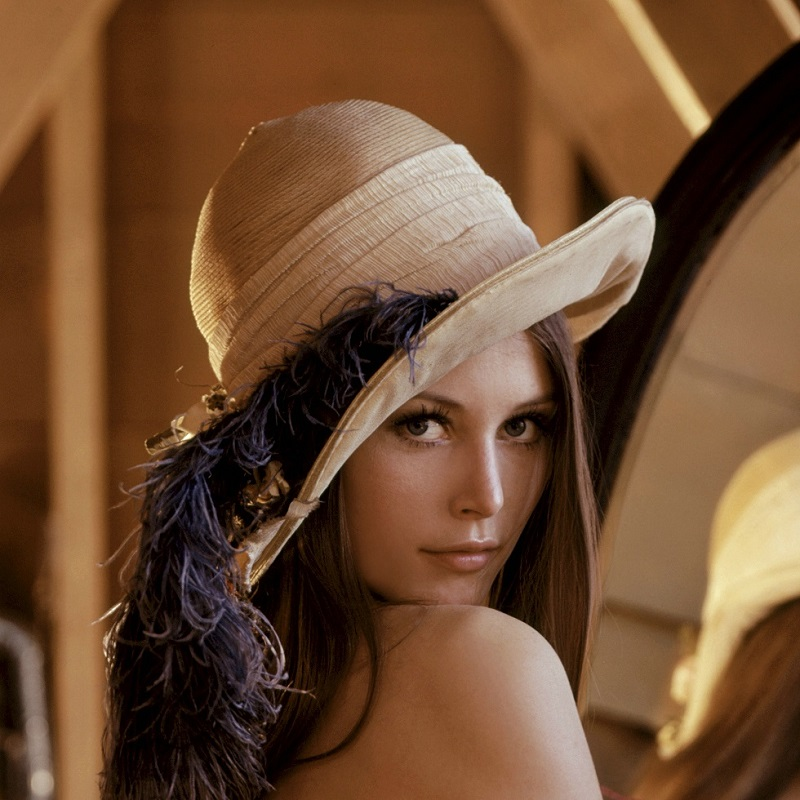
\includegraphics[width=0.25\linewidth]{img/affine_2_src.png}
    }
    \quad\quad\quad\quad
    \subfloat[dst\label{fig-opencv-affine-2-dst}]{
        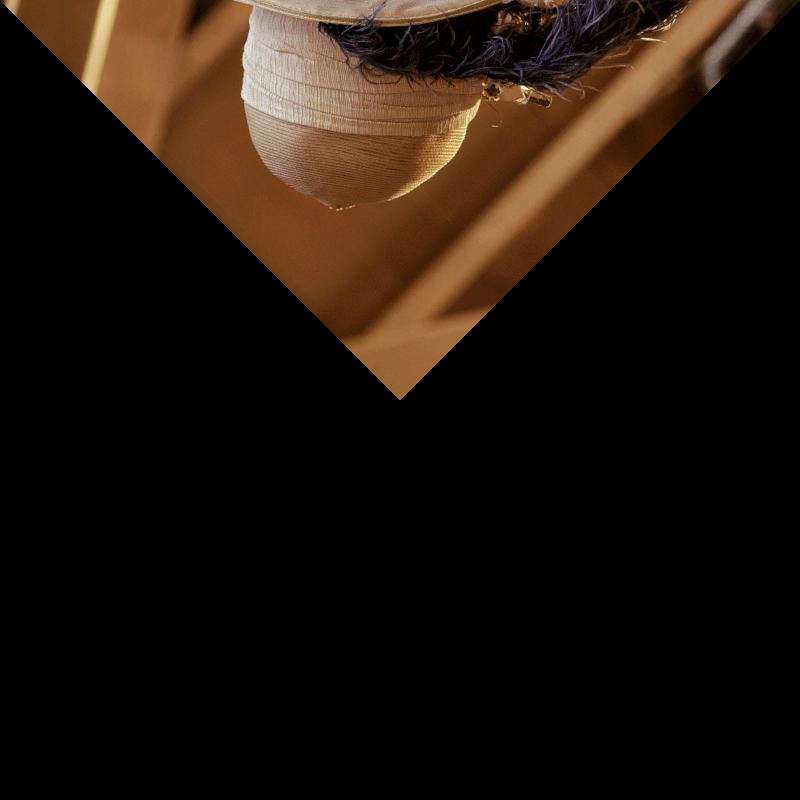
\includegraphics[width=0.25\linewidth]{img/affine_2_dst.png}
    }
    \caption{Abbildung zweier Dreiecke als affine Transformation}
    \label{fig-opencv-affine-2}
\end{figure}
Um die Abbildung zwischen zwei allgemeinen (konvexen) Vierecken darzustellen, muss eine perspektivische Transformation gewählt werden. Schließlich bildet eine affine Transformation parallele Linien wieder auf parallele Linien ab, womit Parallelogramme stets auf Parallelogramme abgebildet werden.

Eine solche perspektivische Transformation lässt sich durch eine $3\times3$ Matrix $\mathbf{P}$ darstellen, welche vier Punkte auf vier andere Punkte abbildet (genau genommen auf ein Vielfaches dieser Punkte), sodass: $$\begin{bmatrix}\lambda_i x_i^\prime\\\lambda_i y_i^\prime\\\lambda_i\end{bmatrix}=\underbrace{\begin{bmatrix}p_{11}&p_{12}&p_{13}\\p_{21}&p_{22}&p_{23}\\p_{31}&p_{32}&p_{33}\end{bmatrix}}_{\mathbf{P}}\cdot\begin{bmatrix}x_i\\y_i\\1\end{bmatrix},1\leq i\leq4$$.

In OpenCV lässt sich diese Matrix mit der Funktion \texttt{cv::getPerspectiveTransform()} finden. Die Funktion \texttt{cv::warpPerspective()} übernimmt dann die eigentliche Transformation des Bildes mit der Matrix.
\chapter{Metriken zur Bildrekonstruktion}\label{ch-metrics}
Um Schiebepuzzles mit Bildern lösen zu können, muss zunächst das Ausgangsbild (als gewünschten Endzustand) bekannt sein. Der erste Schritt ist somit, dieses Bild aus einer Menge von (rechteckigen) Puzzlestücken zu rekonstruieren. Diese Art von Problemstellung erinnert an eine andere Form von Puzzle, welche im englischen Sprachraum als \textit{Jigsaw Puzzle} bezeichnet werden. Abbildung \ref{fig-jig-ex} zeigt ein Beispielpuzzle dieser Art.
\begin{figure}[H]
    \centering
    \subfloat[Ausgangspuzzle\label{fig-jig-ex-1}]{
        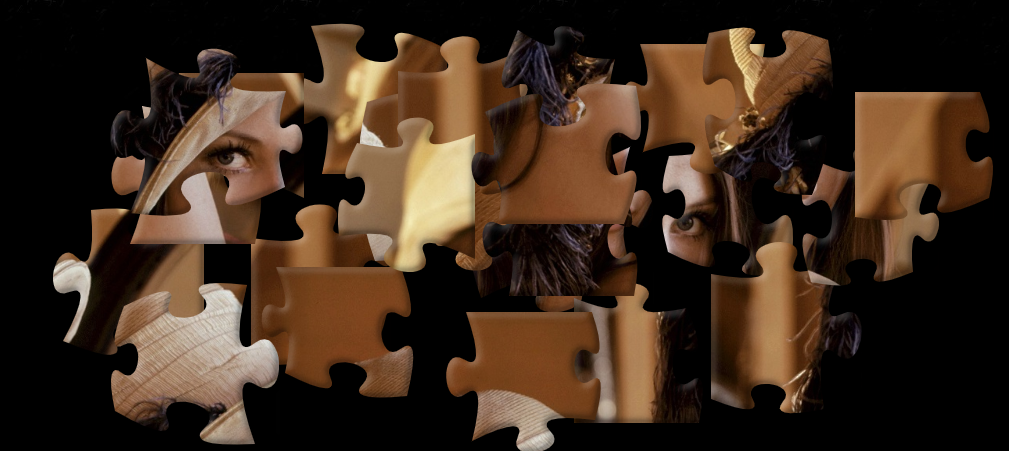
\includegraphics[width=0.70\linewidth]{img/jigex2.png}
    }
    \\
    \subfloat[Teillösung\label{fig-jig-ex-2}]{
        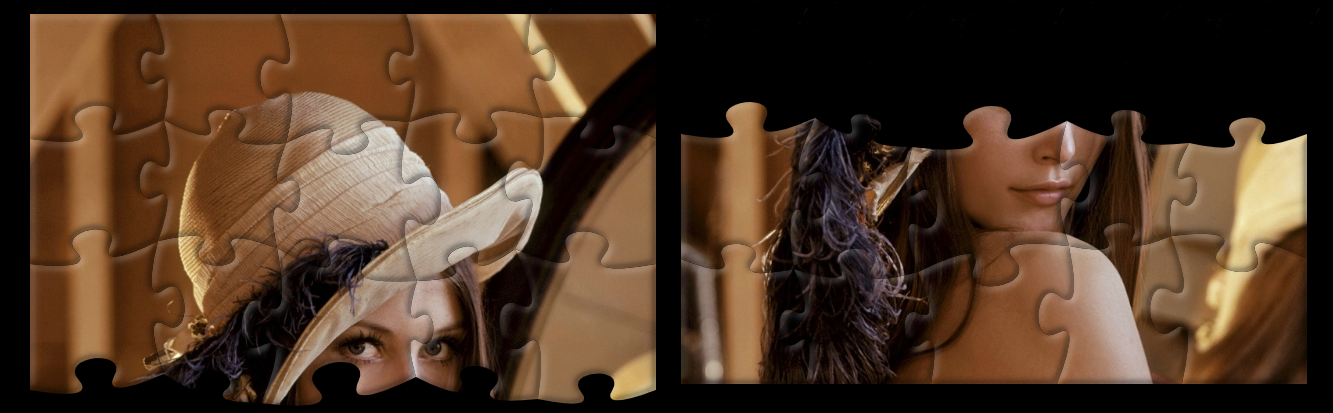
\includegraphics[width=0.60\linewidth,valign=t]{img/jigex3.png}
    }
    \quad
    \subfloat[Lösung\label{fig-jig-ex-3}]{
        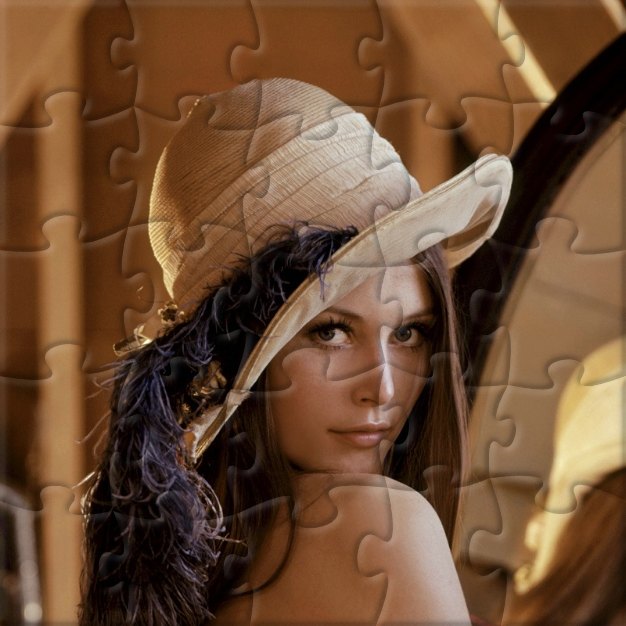
\includegraphics[width=0.30\linewidth,valign=t]{img/jigex1.png}
    }
    \caption{Beispiel eines Jigsaw-Puzzles}
    \label{fig-jig-ex}
\end{figure}
Normalerweise sind die Puzzlestücke dabei speziell geformt (oftmals ähnlich wie in Abb. \ref{fig-jig-ex}). Dies schränkt die Möglichkeiten der gültigen Zusammensetzungen des Puzzles stark ein, besonders da die Möglichkeit besteht zwischen Rahmenstücken und inneren Puzzlestücken zu unterscheiden (Stücke am Rand des Bildes haben mindestens eine glatte Kante). Dadurch entsteht ein Problem, welches sich teilweise nur durch die äußere Form der Puzzlestücke und deren Kompatibilität untereinander lösen lässt. Es gibt sogar Puzzle bei denen diese Information hinreichend ist um das Puzzle vollständig zu lösen (die Stücke selber weisen dann keine weiteren optischen Merkmale auf und sind meist einfarbig).

Mit der Motivation später Schiebepuzzle lösen zu können, muss das Problem auf rechteckige Puzzlestücke verallgemeinert werden. Damit kann weder gesagt werden, ob ein Puzzlestück ein Rahmenstück ist oder sich im inneren des Puzzles befinden muss, noch können Aussagen über die Kompatibilität zweier Puzzlestücke gemacht werden, ohne dabei die Bilder der Puzzlestücke zu analysieren.

Eine noch speziellere Variante von rechteckigen Jigsaw-Puzzles schränkt die Puzzlestücke auf eine quadratische Größe ein. Bei diesen Square Jigsaw Puzzles werden in der Literatur nach \cite{gallagher} zwischen drei Typen unterschieden. Alle Typen haben (sofern nicht anders definiert) Informationen über die Dimensionsgrößen ($m$ Zeilen, $n$ Spalten) des Puzzles. Alle Puzzleteile sind quadratisch (mit der gleichen Seitenlänge) und besitzen Farbinformationen (in Form von einem Bild für jedes Stück). Es gibt exakt $N=m\times n$ Puzzlestücke, womit das Puzzle also keine Lücken oder überschüssige Teile haben wird.

Bei dem Type 1 Square Jigsaw Puzzle ist die Position der Puzzlestücke unbekannt, deren Orientierung jedoch fest und bekannt. Alle möglichen Puzzlestellungen sind dann eine Permutation der vorhandenen Puzzlestücke. Davon gibt es $N!$ verschiedene. Außerdem lassen sich somit zwei Puzzleteile $(x_i,x_j)$ auf vier verschiedene Arten zusammensetzen ($x_i$ kann links, rechts, oben oder unten von $x_j$ platziert werden). Jede Seite von $x_i$ hat nur eine Seite von $x_j$ als möglichen Partner. Das Type 1 Puzzle ist der am meisten untersuchteste Typ von den dreien und hat den Namen \textit{jig swap}\cite{loop} bekommen.

Das Type 2 Puzzle lässt eine unbekannte Orientierung der Puzzleteile zu. Somit lassen die Puzzleteile sich nicht nur anordnen, sondern auch rotieren. Die Anzahl der möglichen Anordnungen des Puzzles vervielfacht sich somit um einen Faktor von $4^N$ auf insgesamt $4^N\cdot N!$. Zwei Puzzlestücke $(x_i,x_j)$ lassen sich nun auf $16$ verschiedene Arten anordnen, da jede Seite von $x_i$ mit jeder Seite von $x_j$ kombiniert werden kann.

Beim Type 3 Puzzle ist die Orientierung zwar unbekannt, die Positionen der Puzzleteile sind jedoch fest und bekannt. Da die Anordnung fest ist und jedes Puzzlestück sich rotieren lässt, hat dieses Puzzle mit $4^N$ möglichen Anordnung die geringste Komplexität. Zwei Puzzlestücke $(x_i,x_j)$ lassen sich auch hier auf $16$ verschiedene Arten kombinieren. Der Unterschied dabei zu Type 1 und Type 2 Puzzles ist jedoch, dass nur die Kompatibilität zwischen Seiten von bereits benachbarten Teilen analysiert werden muss (da die Anordnung fest ist). Bei Type 1 und Type 2 Puzzles kommen für ein Teil $x_i$ alle anderen Teile $x_j,j\neq i$ als mögliche Nachbarn in Frage.

Die Anzahl der möglichen Kombinationen die es gibt, wenn man zwei Seiten von zwei Puzzlestücken vergleichen möchte, ist bereits eine gute untere Schranke für die Laufzeit- und Speicherkomplexität von Algorithmen, welche die Kompatibilität aller Puzzlestücke (in allen möglichen Anordnungen) braucht, um Entscheidungen treffen zu können (um beispielsweise zunächst die Puzzlesteile zu kombinieren, welche von allen die höchste Kompatibilität aufweisen).

Type 1 Puzzle müssen alle Puzzlestücke mit allen anderen Puzzlestücken vergleichen. Da die Kompatibilität zwischen zwei Stücken symmetrisch ist und es $4$ Möglichkeiten gibt die zwei Stücke in einem Type 1 Puzzle anzuordnen ergeben sich somit $$4\binom{N}{2}=2N(N-1)\in\Theta(N^2)$$ Kompatibilitäten die berechnet werden müssen.

Bei Type 2 Puzzle ändert sich lediglich der konstante Faktor vor dem Binomialkoeffizienten von $4$ auf $16$, womit sich auch die Anzahl der berechneten Metriken vervierfach und somit auf $8N(N-1)$ wächst, was weiterhin $\Theta(N^2)$ ist.

Im Gegensatz dazu werden bei Type 3 Puzzles lediglich die Kompatibilitäten zu den benachbarten Puzzlestücken berechnet. Durch die mögliche Rotation der beiden Stücke ergeben sich (wie bei Type 2) $16$ Möglichkeiten pro Paar. Jedes Paar entspricht einer (inneren) Kante im Puzzle (vgl. Abb. \ref{fig-type3}). Die Anzahl der vertikalen Kanten (in der Abbildung rot gekennzeichnet) entspricht $m(n-1)$, die Anzahl der horizontalen Kanten (in der Abbildung grün gefärbt) entspricht dann der Symmetrie nach $n(m-1)$. Damit ergeben sich insgesamt
\begin{align*}
    &16[m(n-1)+n(m-1)]\\
    =&16[2mn-m-n]\\
    =&16(2N-m-n)\in\Theta(N)
\end{align*}
mögliche Kompatibilität, die berechnet werden müssen.
\begin{figure}[H]
    \centering
    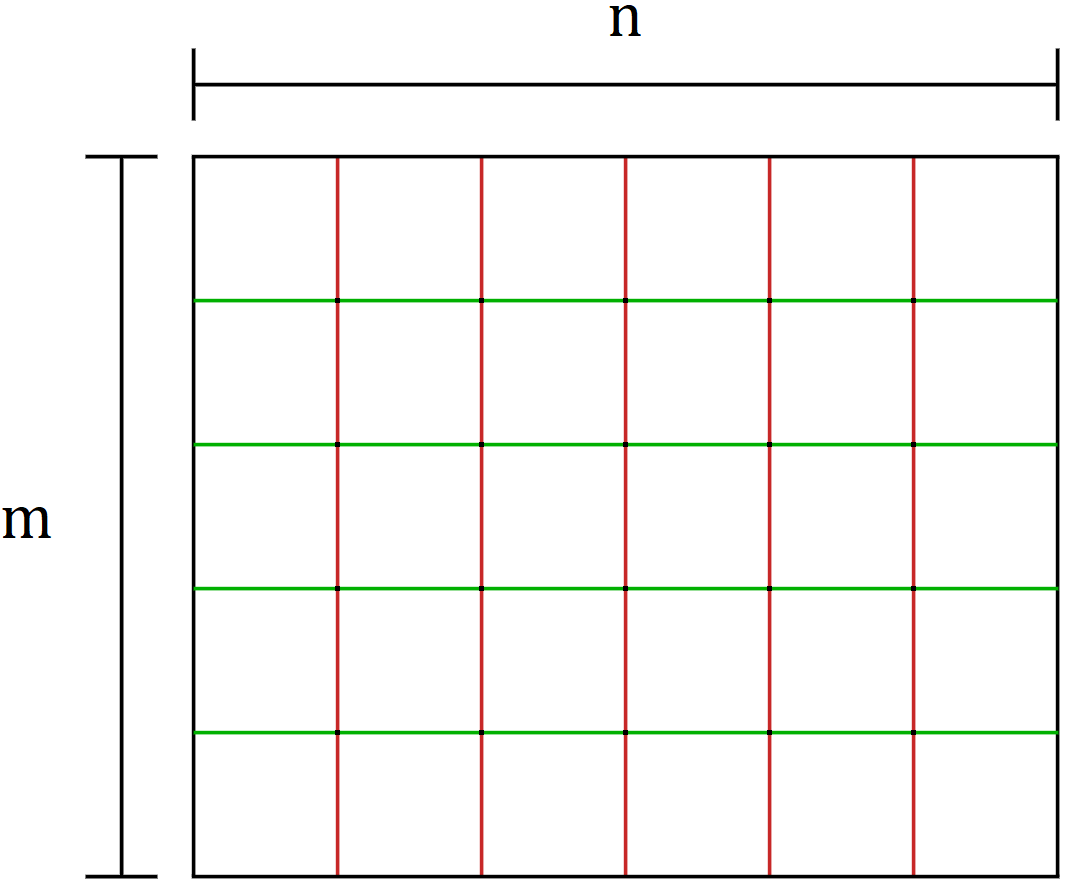
\includegraphics[width=0.60\linewidth]{img/type3.png}
    \caption{Anzahl der Kanten bei einem Type 3 Puzzle}
    \label{fig-type3}
\end{figure}
Es ist zu beachten, dass $N$ bereits quadratisch wächst (bei einem Puzzle mit quadratischen Dimensionen $m=n$). Bei einem $n\times n$ Puzzle ist der Aufwand eines Type 3 Puzzles somit mindestens quadratisch von $n$ abhängig. Bei Type 1 und Type 2 Puzzles wächst dies noch schneller: $\Theta(N^2)=\Theta(n^4)$.

Außerdem sei noch erwähnt, dass mögliche Lösungen beim Type 2 Puzzle aufgrund der erlaubten Rotation (und der Tatsache, dass die Position der Stücke nicht fixiert ist) nicht unbedingt eindeutig sind. Selbst wenn ein Algorithmus es schafft das Bild so zu rekonstruieren, dass jede Seite eines Puzzlestückes den richtigen Partner hat, kann es sein, dass das Gesamtbild jedoch rotiert ist.

Im weiteren Verlauf dieser Arbeit werden hauptsächlich Type 1 Puzzles betrachtet, da Schiebepuzzle sowieso keine Rotation zulassen. Abbildung \ref{fig-jigswap} zeigt ein $8\times 8$ Type 1 Puzzle.
\begin{figure}[H]
    \centering
    \subfloat[Permutiertes Puzzle\label{fig-jigswap-1}]{
      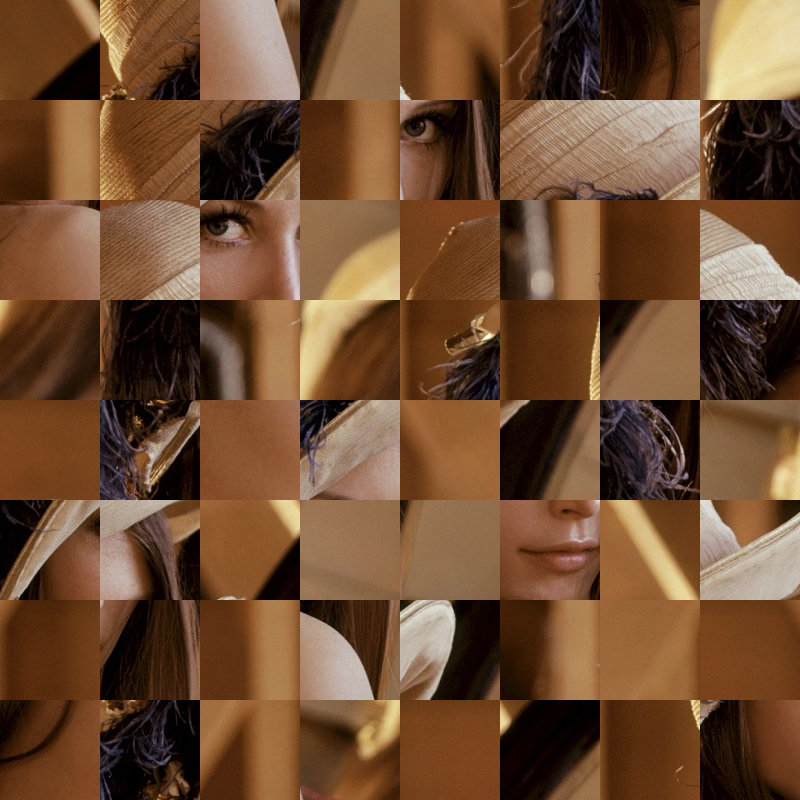
\includegraphics[width=0.30\linewidth]{img/jigswap2.png}
    }
    \quad\quad\quad\quad
    \subfloat[Gelöstes Puzzle\label{fig-jigswap-2}]{
      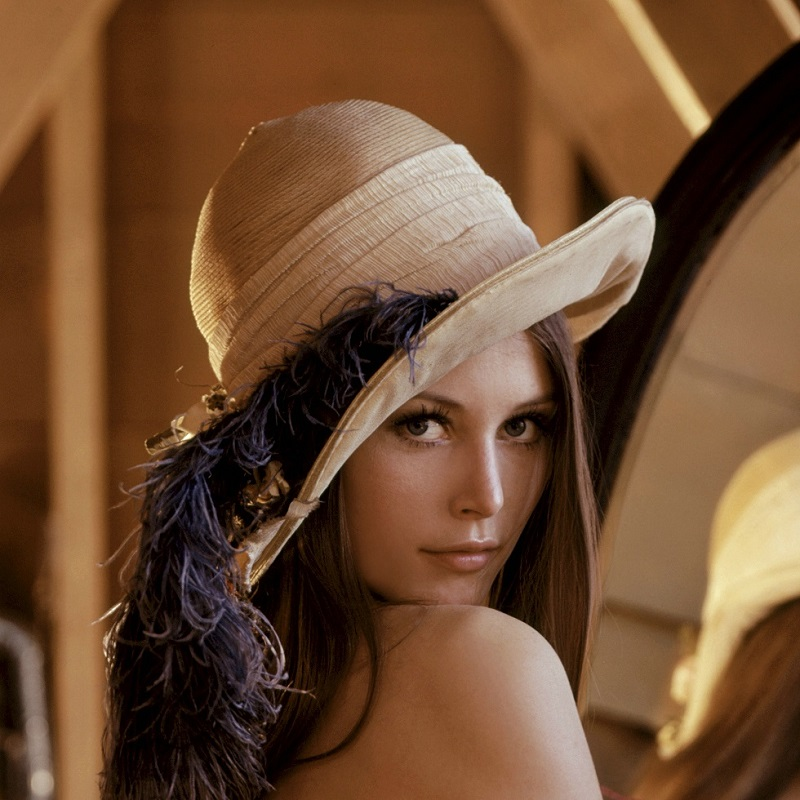
\includegraphics[width=0.30\linewidth]{img/jigswap1.png}
    }
    \caption{Beispiel eines Type 1 Puzzles}
    \label{fig-jigswap}
\end{figure}
Zur Rekonstruktion des Bildes werden Kompatibilitätsmetriken betrachtet, welche später als Information vom eigentlichen Algorithmus verwendet werden, um Entscheidungen zu treffen, welche Puzzlestücke miteinander kombiniert werden sollen und welche nicht.

Genau genommen werden im Folgenden eher Metriken (Distanzfunktionen) betrachtet, die genau das Gegenteil von der Kompatibilität zweier Puzzlestücke darstellen. Den Begriff der Kompatibilität wurde jedoch in \cite{pomeranz} eingeführt und wird seitdem in weiterer Literatur verwendet.
\section{$(L_p)^q$ Norm}\label{section-norm}
Um Aussagen über die Kompatibilität bzw. die Unähnlichkeit (mit Hilfe einer Distanzfunktion) zweier Puzzlestücke zu machen, muss zunächst geklärt werden, wie die Distanz zweier Pixel beschrieben werden kann. Welche Pixel wirklich miteinander verglichen werden beim Vergleich zweier Puzzlestücke ist schließlich erst dann relevant, wenn Möglichkeiten bestehen, die Unähnlichkeit von zwei Pixeln anzugeben.

Da weiterhin Farbbilder aus dem (OpenCV übglichen) BGR-Raum betrachtet werden und somit jeder Pixel drei Channel (mit je 8 Bit) hat, lässt sich ein Pixel als einen Vektor aus dem Raum $[0,256)^3$ auffassen. Damit lässt sich eine Norm $\|\cdot\|:[0,256)^3\rightarrow[0,\infty)$ definieren. Mit einer Norm lässt sich aber mit $d(\vec{u},\vec{v})\coloneqq\|\vec{u}-\vec{v}\|$ eine Metrik einführen.

Die aus der Mathematik bekannte $L_p$ Norm mit $$L_p(\vec{v})=\|\vec{v}\|_p\coloneqq\sqrt[p]{\sum_{i=1}^{n}|v_i|^p},p\in\mathbb{R}^{\geq1}$$ liegt dabei am nächsten. Besonders die $L_2$ Norm (euklidische Norm) oder die $L_1$ Norm (Taxicab Norm oder Manhatten Norm) würden in Frage kommen. In \cite{pomeranz} wurde jedoch für Jigsaw Puzzles mit der $(L_p)^q$ Norm eine weitere (allgemeinere) Norm eigeführt. Die $(L_p)^q$ Norm berechnet sich zu $$(L_p)^q[\vec{v}]=\|\vec{v}\|_p^q\coloneqq \sqrt[\leftroot{-2}\uproot{5}\frac{p}{q}]{\sum_{i=1}^{n}|v_i|^p}$$.

Die $(L_p)^q$ Norm ist damit die mit $q$ potenzierte $L_p$ Norm: $(L_p)^q[\vec{v}]\coloneqq(L_p[\vec{v}])^q$. Auch in \cite{pomeranz} (empirisch) gezeigt wurde, dass besonders $p=\frac{3}{10}$ und $q=\frac{1}{16}$ gute Ergebnisse liefern.
\section{Dissimilarity-Based Compatibility (DBC)} \label{section-dbc}
Die erste Metrik beschrieben in \cite{pomeranz} ist die Dissimilarity-Based Compatibility (DBC). Diese summiert die Distanzen zweier Puzzlestücke entlang einer Kante auf. Da es für Type 1 Puzzle vier verschiedene Möglichkeiten gibt, zwei Stücke $x_i$ und $x_j$ anzuordnen, wird zunächt eine numerische Konstante $r\in\{0,1,2,3\}$ definiert, die diesen Zusammenhang darstellt.
\begin{table}[H]
    \centering
    \begin{tabular}{c|c|c|c}
        $r=0$ & $r=1$ & $r=2$ & $r=3$\\
        \hline
        \begin{tikzpicture}
            \draw (0,0) rectangle (1,1) node[midway] {$x_i$};
            \draw (1,0) rectangle (2,1) node[midway] {$x_j$};
        \end{tikzpicture}&
        \begin{tikzpicture}
            \draw (0,0) rectangle (1,1) node[midway] {$x_j$};
            \draw (0,1) rectangle (1,2) node[midway] {$x_i$};
        \end{tikzpicture}&
        \begin{tikzpicture}
            \draw (0,0) rectangle (1,1) node[midway] {$x_j$};
            \draw (1,0) rectangle (2,1) node[midway] {$x_i$};
        \end{tikzpicture}&
        \begin{tikzpicture}
            \draw (0,0) rectangle (1,1) node[midway] {$x_i$};
            \draw (0,1) rectangle (1,2) node[midway] {$x_j$};
        \end{tikzpicture}
    \end{tabular}
    \caption{Räumlicher Zusammenhang zweier Puzzlestücke}
    \label{tbl-spatial-relation}
\end{table}
Die DBC entlang einer Kante, die beim Zusammensetzen zweier Puzzlestücke entsteht, wird dann mit $D(x_i,x_j,r)$ bezeichnet. Da diese Metrik symmetrisch ist gilt außerdem $D(x_i,x_j,r)=D(x_j,x_i,r^\prime)$. Wobei $r^\prime$ die inverse Relation der beiden Puzzlestücke darstellt und sich zu $$r^\prime=(r+2)\bmod4$$ berechnet.

Als Referenzstellung der beiden Puzzleteile wird im weiteren Verlauf $r=0$ verwendet ($x_i$ befindet sich also links von $x_j$). Andere Stellungen lassen sich entweder ähnlich berechnen (lediglich durch das Vertauschen der Dimensionen oder durch das Vertauschen von $i$ und $j$) oder sogar gleich berechnen, sofern die beiden Puzzlestücke zuvor entsprechend rotiert wurden.

Diese DBC zweier Puzzlestücke $x_i(x,y)$ und $x_j(x,y)$ mit Höhe $h$ und Breite $w$ und basierend auf einer Norm $\|\cdot\|$ berechnet sich dann zu:
\begin{align} \label{eq-dbc}
    D(x_i,x_j,0)=\sum_{k=0}^{h-1}\|x_i(w-1,k)-x_j(0,k)\|
\end{align}
.

Da diese Distanz bei rechteckigen Puzzlestücken die kürzeren Seiten generell bevorzugt (die Summanden sind stets positiv, womit selbst gute Kanten bei vielen Summanden große Werte liefern), kann diese Distanz noch durch die Anzahl der Summanden bzw. die Länge der Seite $K$ (bei $r=0$ beispielsweise die Höhe der Puzzlestücke) dividiert werden: $$\bar{D}(x_i,x_j,r)=\frac{1}{K}\cdot D(x_i,x_j,r)$$.

Um diese Distanz gegebenenfalls noch auf das Intervall $[0,1]$ zu normalisieren, lässt sich die durchschnittliche Distanz (pro Summand) durch die maximale Distanz $d_{max}$ zwischen zwei Pixel dividieren. Diese maximale Distanz hängt von der gewählten Norm ab. Bei der euklidischen Norm ist dies beispielsweise $d_{max}=\sqrt{255^2+255^2+255^2}=\sqrt{3\cdot255^2}=\sqrt{3}\cdot255$.

Damit lässt sich nun die Kompatibilität zweier Puzzlestücke als die Gegenwahrscheinlichkeit dieser relativen Distanz definieren:$$C(x_i,x_j,r)\coloneqq 1-\frac{\bar{D}(x_i,x_j,r)}{d_{max}}$$.

Die DBC bietet eine simple Möglichkeit die Kompatibilität (oder Distanz) zwischen zwei Puzzlestücken zu berechnen. Die Berechnung einer solchen Distanz bezüglich einer Kante ist linear in der Länge dieser Kante $\Theta(K)$ (Höhe oder Breite der Puzzlestücke). Ein Nachteil ist, dass lediglich die äußersten Pixel eines Puzzlestückes betrachtet werden. Dadurch werden Farbübergänge, die zwar im Gesamtbild Sinn ergeben, an den Kanten als harsch angesehen, da diese dort für große Distanzen sorgen.
\section{Prediction-Based Compatibility (PBC)}\label{section-pbc}
Um neben den Randpixeln auch noch die Informationen von deren (inneren) benachbarten Pixeln nutzen zu können, wird bei der Prediction-Based Compatibility (PBC) das Bild eines Puzzlestückes um einen Pixel in jede Richtung erweitert. Diese approximierten Pixel einer Seite werden dann anstatt den eigentlichen Pixeln dieser Seite (wie es bei der DBC der Fall ist) in der Distanzberechnung verwendet. Es wird also die Distanz zwischen einem approximierten Pixel in einem Puzzlestück und einem echten Pixel in einem anderen Puzzlestück ermittelt.

Zur Approximierung der Farbwerte lässt sich ein Bild $I$ mit der Breite $w$ und der Höhe $h$ im BGR-Farbraum wieder als vektorwertige Funktion $\vec{I}(\vec{x}):[0,w)\times[0,h)\rightarrow[0,256)^3$ betrachten. Es wird eine lineare Approximierung nach Taylor gewählt. Um eine Entwicklungsstelle $\vec{x}_0$ gilt dann $$\vec{I}(\vec{x})\approx\vec{I}(\vec{x}_0)+J_I(\vec{x}_0)\cdot(\vec{x}-\vec{x_0})$$. Wobei mit $J_I(\vec{x}_0)$ die Jacobi-Matrix (ausgewertet an der Entwicklungsstelle $\vec{x}_0$) gemeint ist. Die Jacobi-Matrix fasst alle partiellen Ableitungen der Funktion zusammen (die Komponenten von $I$ werden entsprechend der Farbchannel als $b$, $g$ und $r$ bezeichnet): $$J_I=\begin{bmatrix}\frac{\partial b}{\partial x}&\frac{\partial b}{\partial y}\\\frac{\partial g}{\partial x}&\frac{\partial g}{\partial y}\\\frac{\partial r}{\partial x}&\frac{\partial r}{\partial y}\end{bmatrix}$$.

Um die einzelnen Ableitungen numerisch zu bestimmen, werden finite Differenzen verwendet. Dabei wird unterschieden zwischen dem Forward-Differenzenquotienten $\Delta_F[f](x)$, Backward-Differenzenquotienten $\Delta_B[f](x)$ und Central-Differenzenquotienten $\Delta_C[f](x)$.
\begin{align*}
    \Delta_F[f](x) &= \frac{f(x+h)-f(x)}{h}\\
    \Delta_B[f](x) &= \frac{f(x)-f(x-h)}{h}\\
    \Delta_C[f](x) &= \frac{\Delta_F[f](x)+\Delta_B[f](x)}{2}\\
                   &= \frac{f(x+h)-f(x-h)}{2h}
\end{align*}
Der Central-Differenzenquotient ist damit also das arithmetische Mittel vom Forward-Differenzenquotienten und vom Backward-Differenzenquotienten. Da die Ableitung einer Funktion $f$ an einer Stelle $x$ gerade der Grenzwert dieser Quotienten darstellt, für die $h\rightarrow0$, werden zur numerischen Berechnung kleine $h\neq0$ gewählt. Die Koordinaten $(x,y)$ eines Bildes können jedoch nur diskrete Werte annehmen, womit das kleinstmögliche $h$ somit $h=1$ ist. Das Aufstellen der Differenzenquotienten für vektorwertige Funktionen lässt sich analog zum skalaren Beispiel konstruieren (wobei die Funktionsdifferenz im Zähler dann eine Vektordifferenz ist, anders gesagt wird der Differenzenquotient für jede Komponente gebildet). Für Funktionen, die von mehreren Variablen abhängig sind, entsprechen die Differenzenquotienten dann einer Approximierung der partiellen Ableitungen, wobei lediglich der Parameter variiert wird, nach dem abgeleitet werden soll. Die restlichen Parameter werden konstant gehalten.

Als Beispiel lässt sich somit ein Bild an den Rändern erweitern, indem der nächstgelegene Pixel als Entwicklungsstelle für die lineare Approximierung genommen wird. In Abbildung \ref{fig-pred} wird gezeigt, wie ein Bild sowohl nach oben als auch nach rechts um jeweils einen Pixel erweitert wird.

Ein Pixel am (erweiterten) rechten Rand (in der Zeile $y$) des Bildes hat die Koordinaten $(w,y)$. Als Entwicklungsstelle wird der links benachbarte Pixel mit den Koordinaten $(w-1,y)$ gewählt. Der Farbwert des neuen (erweiterten) Pixels lässt sich dann mit
\begin{align} \label{eq2}
    \vec{I}(w,y) &= \vec{I}(w-1,y) + \begin{bmatrix}
        \frac{\partial \vec{I}}{\partial x} &
        \frac{\partial \vec{I}}{\partial y}
    \end{bmatrix}
    \biggr \rvert_{(x,y)=(w-1,y)} \cdot
    \left( \begin{bmatrix}
        w \\
        y
    \end{bmatrix} - \begin{bmatrix}
        w-1 \\
        y
    \end{bmatrix} \right),&\forall y:0\leq y<h \nonumber \\
    &= \vec{I}(w-1,y) + \begin{bmatrix}
        \vec{I}_x(w-1,y) & \vec{I}_y(w-1,y)
    \end{bmatrix} \cdot \begin{bmatrix}
        1 \\
        0
    \end{bmatrix} \nonumber \\
    &= \vec{I}(w-1,y) + \vec{I}_x(w-1,y)
\end{align}
approximieren.

Bei der numerischen Approximierung der partiellen Ableitung von $\vec{I}$ entlang der $x$-Achse kommt ausschließlich der Backward-Differenzenquotient in Frage. Dies liegt daran, dass die Pixel mit einer $x$-Koordinate von $w-1$ sich in der letzten Spalte des Bildes befinden und somit entlang der $x$-Achse keinen rechts benachbarten Pixel haben. Damit ergibt sich:
\begin{align} \label{eq3}
    \vec{I}_x(w-1,y) &= \Delta_B\left[\vec{I}\right](w-1,y) \nonumber \\
    &= \frac{\vec{I}(w-1,y)-\vec{I}(w-1-h,y)}{h} \nonumber \\
\shortintertext{Mit $h=1$ folgt}
    \vec{I}_x(w-1,y) &= \vec{I}(w-1,y)-\vec{I}(w-2,y)
\end{align}
Insgesamt ergibt sich mit \ref{eq2} und \ref{eq3} die vollständige Formel zu Berechnung des erweiterten Randes vom Bild.
\begin{align} \label{eq4}
    \vec{I}(w,y)=2\vec{I}(w-1,y)-\vec{I}(w-2,y)
\end{align}
Die Formulierung einer solchen Approximierung für Pixel an anderen Seiten des Bildes lässt sich ähnlich angeben. Lediglich bei der Approximierung der Pixel in einer (neuen) Ecke des Bildes müssen beide partiellen Ableitungen approximiert werden (als Entwicklungsstelle wird die alte Ecke des Bildes genommen, womit sowohl ein Schritt entlang der x-Achse, also auch einen Schritt entlang der y-Achse gegangen wird).

Außerdem ist noch zu beachten, dass mit der reinen Berechnung nach \ref{eq4} noch nicht sichergestellt ist, dass die Channel des neuen Pixels sich auch wieder in dem Wertebereich $[0,256)$ befinden. Es gilt also zu beachten, dass die Berechnung keine modulare Arithmetik verwenden sollte (dazu sollte die Berechnung in einem größeren Vorzeichen behafteten Datentyp stattfinden). Um die Werte danach wieder auf das Intervall $[0,256)$ zu bringen, sollte dann unbedingt der in \ref{section-sat} angesprochene \texttt{cv::saturate\_cast<>()} verwendet werden.

Der folgende Ausschnitt an Quelltext zeigt, wie die Berechnung nach \ref{eq4} mit einem Quellbild \texttt{src} und einem Zielbild \texttt{dst} in OpenCV umgesetzt werden kann.
\begin{lstlisting}[caption=Lineare Approximierung (nach Taylor) von Pixel am rechten Bildrand, label=lst-pred-sat]
for (size_t row = 0; row < src.rows; row++)
{
    for (size_t ch = 0; ch < 3; ch++)
    {
        dst.at<cv::Vec3b>(row, src.cols)[ch] =
            cv::saturate_cast<cv::uchar>(
                  2 * dst.at<cv::Vec3b>(row, src.cols - 1)[ch]
                -     dst.at<cv::Vec3b>(row, src.cols - 2)[ch]
            )
        ;
    }
}
\end{lstlisting}
Um den \texttt{cv::saturate\_cast<>()} geeignet anwenden zu können, werden die Pixel im Quelltext Channel für Channel durchgegangen (Schleife in Zeile 3). Außerdem wird mit der Multiplikation der numerischen Konstante $2$ in Zeile 7 die komplette Berechnung implizit zu einer Berechnung mit Integer Werten. Wäre dies hier nicht der Fall, würde auch die Saturierung des berechneten Wertes nichts daran ändern, dass bereits bei der Berechnung selber gegebenenfalls Over- oder Underflows aufgetreten sind.

Abbildung \ref{fig-pred} zeigt neben dem Ausgangsbild und der oberen rechten Ecke dieses Bildes, zwei Varianten zur Berechnung der Approximierung.

In \ref{fig-pred-nosat} wurde der Saturate-Cast weggelassen, wodurch der (zunächst richtig) berechnete Wert bei der Zuweisung an einen kleineren Datentypen die Informationen in den höheren Bits verliert. Als Ergebnis entstehen einzelne Pixel, die stark vom eigentlichen Bildverlauf abweichen. Suggerieren zwei benachbarte Pixel etwa einen immer dunkler werdeden Farbverlauf, so kann es vorkommen, dass der approximierte Pixel als so dunkel angenommen wird, dass die Werte der Channel bei der Berechnung negativ werden. Diese Annahme ist nicht falsch. Ein impliziter Cast zu einem \texttt{uchar} bewirkt dann jedoch, dass die Channel sehr große Werte annehmen. Das bereits beschriebene Clamping vom Saturate-Cast verhindert dies, sodass ein überaus dunkler Pixel in jedem Channel gegebenenfalls auf den dunkelsten Wert (welcher $0$ entspricht) gesetzt wird. Die gleiche Berechnung mit einem Saturate-Cast liefert, wie in \ref{fig-pred-sat} zu sehen ist, eine zum Farbverlauf passende und somit realistisch aussehende Approximierung der neuen Randpixel.
\begin{figure}[H]
    \centering
    \subfloat[Originalbild\label{fig-pred-orig}]{
      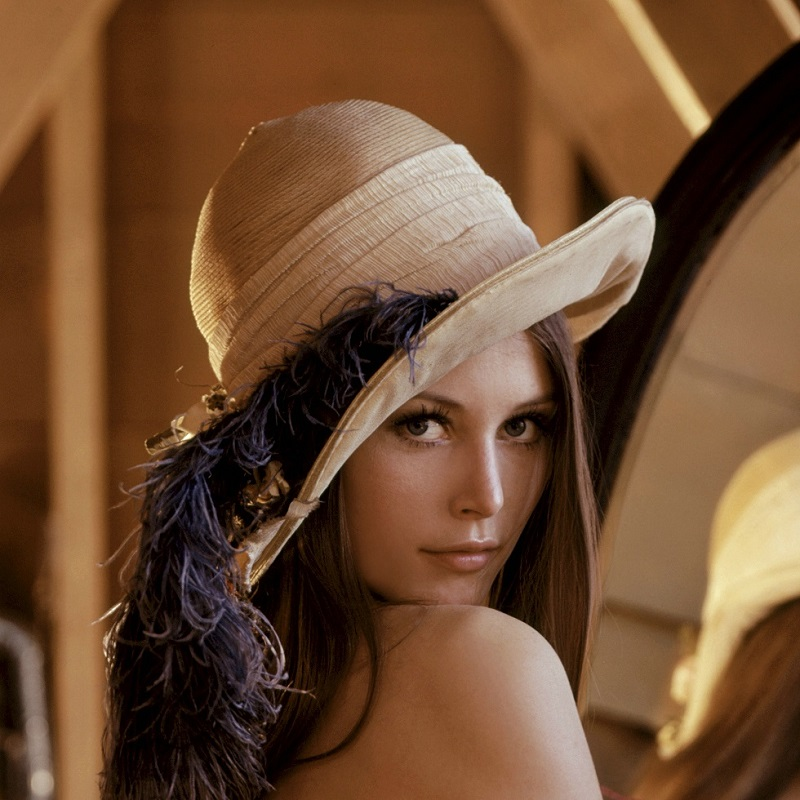
\includegraphics[width=0.40\linewidth,valign=t]{img/linear_orig.png}
    }
    \quad\quad
    \subfloat[Obere rechte Ecke im Originalbild\label{fig-pred-orig2}]{
      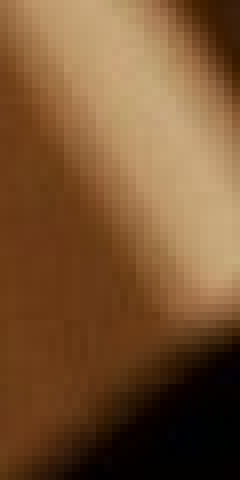
\includegraphics[width=0.20\linewidth,valign=t]{img/linear_orig2.png}
    }
    \\
    \subfloat[Berechnung ohne Saturierung\label{fig-pred-nosat}]{
        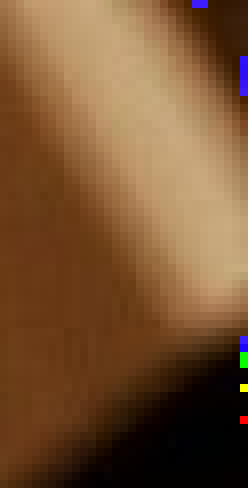
\includegraphics[width=0.20\linewidth]{img/linear_nosat.png}
    }
    \quad\quad\quad\quad\quad\quad\quad\quad
    \subfloat[Berechnung mit Saturierung\label{fig-pred-sat}]{
        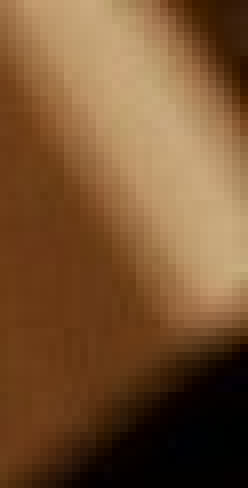
\includegraphics[width=0.20\linewidth]{img/linear_sat.png}
    }
    \caption{Lineare Approximierung der Pixel am rechten und am oberen Bildrand}
    \label{fig-pred}
\end{figure}
Um diese Art der Approximierung nun zu nutzen um die Kompatibilität zweier Puzzlestücke herauszufinden, wird ähnlich wie in \ref{section-dbc} vorgegangen. Als Referenzstellung wird wieder $r=0$ gewählt, womit sich ein Puzzlestück $x_i$ links von einem anderen Puzzlestück $x_j$ befindet. Dabei wird die Berechnung diesmal jedoch in zwei Teile eingeteilt. Es wird zunächst die Distanz betrachtet, die entsteht wenn man die rechte Seite von $x_i$ approximiert und mit den (echten) Pixeln der linkten Seite von $x_j$ vergleicht. Diese Distanz $D_L$ berechnet sich dann analog zu der DBC in \ref{eq-dbc}. Der einzige Unterschied besteht darin, dass die approximierte Spalte an Pixeln von $x_i$ genommen wird. In der Formel aus \ref{eq-dbc} wird also das $x_i(w-1,k)$ zu einem $x_i(w,k)$ geändert, was für die Pixel in der (nicht existierenden, aber approximierten) Spalte von $x_i$ steht. Dann ergibt sich:
\begin{align}\label{eq-DL}
    D_L(x_i,x_j,0)&=\sum_{k=0}^{h-1}\|x_i(w,k)-x_j(0,k)\| \nonumber \\
\shortintertext{Entsprechend der Approximierung in \ref{eq4} lässt sich $x_i(w,k)$ aber als die Linearkombination zweier echten Pixel von $x_i$ berechnen}
    D_L(x_i,x_j,0)&=\sum_{k=0}^{h-1}\|2x_i(w-1,k)-x_i(w-2,k)-x_j(0,k)\|
\end{align}
Um weiterhin garantieren zu können, dass die Distanz zwischen zwei Puzzlestücken symmetrisch ist, wird die Gesamtdistanz zweier Puzzlestücke als die Summe beider Distanzen der Approximierungen gebildet. Dazu wird nun $D_R(x_i,x_j,0)$ ähnlich wie in \ref{eq-DL} berechnet.
\begin{align}\label{eq-DR}
    D_R(x_i,x_j,0)&=\sum_{k=0}^{h-1}\|x_i(w-1,k)-2x_j(0,k)+x_j(1,k)\|
\end{align}
Wurden beide Seiten berechnet, so lässt sich die gesamte Distanz zu $D(x_i,x_j,r)=D_L(x_i,x_j,r)+D_R(x_i,x_j,r)$ berechnen. Damit ist sichergestellt, dass weiterhin der Symmetrie nach $D(x_i,x_j,r)=D\left(x_i,x_j,\left(r+2\right)\bmod4\right)$ gilt.

Da ähnlich wie bei der DBC in \ref{section-dbc} die Distanzen entlang einer Kante aufsummiert werden, ist die Berechnung einer Distanz linear in der Länge dieser Kante. Bei der PBC kommen entsprechend noch zusätzliche Berechnung zur Approximierung der Pixel dazu. Um die Anzahl der konstanten Schritte möglichst minimal zu halten (im Austausch von zusätzlichem Speicherplatz), lassen sich die approximierten Seiten eines Puzzlestückes nur einmal initial berechnen und dann zwischenspeichern. Damit müssen für jedes der $N$ Puzzlestücke zwei horizontale Kanten der Breite $w$ (oben und unten) und zwei vertikale Kanten der Höhe $h$ (links und rechts) abgespeichert werden. Insgesamt müssen damit $2N(w+h)$ Pixel berechnet und abgespeichert werden (alle jeweils mit drei Channel).
\section{Dynamic Time Warping (DTW)}\label{section-dtw}
Eine weitere Methode zur Berechnung der Gesamtdistanz zwischen zwei Puzzlestücken wurde in \cite{hungarian} beschrieben. Intuitiv betrachtet lässt sich vermuten, dass der Vergleich zweier Pixel sich nicht nur auf unmittelbar benachbarte Pixel entlang einer Achse (beispielsweise linke und rechte Nachbarn) beschränken sollte.

Abbildung \ref{fig-dtw-ex} zeigt als Beispiel zwei $8\times1$ Bildränder: $R$ (etwa der rechte Bildrand eines Puzzlestückes $x_i$) und $S$ (der linke Rand eines anderen Puzzlestückes $x_j$). Diese sollen beispielsweise nach \ref{section-dbc} mit der DBC verglichen werden. Wird als Norm die $L_1$ Norm gewählt (Summe der absoluten Differenzen oder auch Manhatten oder Taxicab-Norm), ergibt sich nach dem aufsummieren dieser $8$ Distanzen eine Gesamtdistanz von $2246$.
\begin{figure}[H]
    \centering
    \subfloat[$R$\label{fig-dtw-ex-a}]{
      
\includegraphics[width=0.06\linewidth]{img/dtw_ex_a.png}
    }
    \quad\quad\quad\quad
    \subfloat[$S$\label{fig-dtw-ex-b}]{
      
\includegraphics[width=0.06\linewidth]{img/dtw_ex_b.png}
    }
    \caption{Direkte Zuordnung der Pixel}
    \label{fig-dtw-ex}
\end{figure}
Die Farben in Beispiel \ref{fig-dtw-ex} suggerieren bereits, dass eine andere Zuordnung, welche nicht nur ausschließlich direkt benachbarte Pixel vergleicht, eine geringere Distanz ergeben könnte. So würde beispielsweise das Verschieben von $S$ um einen Pixel nach unten dafür sorgen, dass viele ähnliche Pixel (blau mit blau und grün mit grün) verglichen werden könnte.

Ein Algorithmus der dieses Problem behandelt ist der Dynamic Time Warping (DTW) Algorithmus. Ursprünglich wurde der Algorithmus entwickelt, um die best mögliche Zuordnung (die Zuordnung mit der geringsten Distanz bzw. mit der größten Ähnlichkeit) von zwei zeitabhängigen Sequenzen zu bestimmen (die nicht zwingend gleicher Länge sein müssen). Möchte man beispielsweise Aussagen über die Ähnlichkeit zweier Audiosignale machen, in denen zwei verschiedene Personen die gleiche Sequenz von Wörtern vorlesen (ein Anwendungsbeispiel aus dem Bereich der automatische Spracherkennung), so würde ein direkter Vergleich der beiden Signale auf zwei grundlegende Probleme stoßen: Werden ausschließlich die Frequenzen verglichen, die in den Signalen am gleichen Zeitpunkt $t$ auftreten, so müsste vorausgesetzt werden, dass die beiden Signale die gleiche Länge $T$ haben, was aufgrund der unterschiedlichen Sprachgeschwindigkeit von Menschen sehr unwahrscheinlich ist. Und selbst wenn beide Signale eine gleiche Länge aufweisen, so sorgt genau diese Sprachgeschwindigkeit dafür, dass gegebenenfalls ein Signal zeitlich immer leicht verschoben ist. Somit würden zwei ähnliche Signale als komplett verschieden anerkannt werden, weil bei der Zuordnung der Frequenzen nicht beachtet wird, dass gleiche Frequenzen zeitverschoben auftreten können. Abbildung \ref{fig-dtw-vs} zeigt zwei Beispiel Matchings einer zeitabhängigen Sequenz. Eine direkte Zuordnung (euklidisches Matching) sorgt dafür, dass zeitlich verschobene aber ähnliche Frequenzen nicht einander zugeordnet werden können. Der DTW-Algorithmus findet das beste Matching, indem die Sequenzen so \textit{verzerrt} werden, dass diese Zuordnung der ähnlichen Frequenzen möglich wird.
\begin{figure}[H]
    \centering
    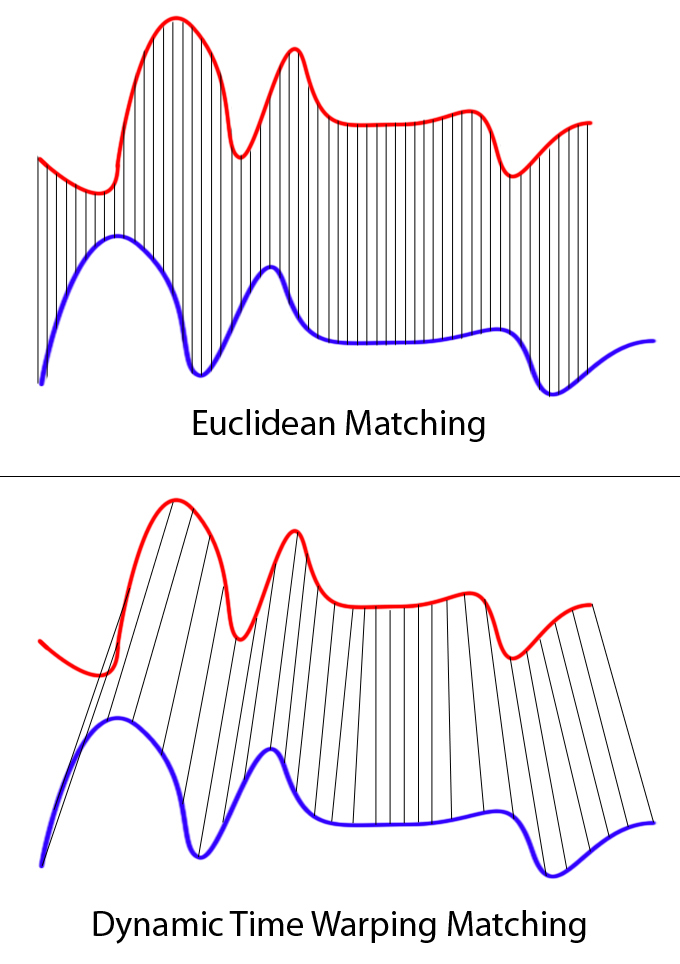
\includegraphics[width=0.60\linewidth]{img/eu_vs_dtw.jpg}
    \caption{Euclidean Matching im Vergleich mit DTW}
    \caption*{Quelle: Wiki Commons: File:Euclidean vs DTW.jpg (\url{https://commons.wikimedia.org/wiki/File:Euclidean_vs_DTW.jpg})}
    \label{fig-dtw-vs}
\end{figure}
Im Gegensatz zu zeitabhängigen Sequenzen (welche ein Beispiel für stetige Sequenzen sind) ist die Zuordnung zwischen zwei Pixelsequenzen diskret, da es nur eine endliche Anzahl an Indizes gibt. Bevor der Algorithmus selber beschrieben werden kann, sollte festgelegt werden, welche Eigenschaften eine Zuordnung aufweisen muss um gültig zu sein (bzw. welche Matchings zulässig sind).

Es werden zwei Sequenzen $R=(r_1,\dots,r_m)$ und $S=(s_1,\dots,s_n)$ betrachtet, mit entsprechenden Längen $|R|=m$ und $S=n$ (im konkreten Fall, wo $R$ und $S$ Seitenränder von Puzzlestücken sind gilt natürlich $m=n$). Auf den Elementen der Sequenz sei eine Metrik bzw. Distanzfuntkion $d(r_i,r_j)$ definiert. Bei den Bildpunkten lässt sich die Matrik mit einer Norm $\|\cdot\|$ nach \ref{section-norm} als $d(r_i,r_j)=\|r_i-r_j\|$ definieren. Gesucht ist die minimale Gesamtdistanz $D$ als Summe einzelner Distanzen durch das Matching jeweils zweier Elemente aus den Sequenzen $D(R,S)=\sum_{i,j}d(r_i,r_j)$. Dieses Matching muss folgende Eigenschaften beachten:
\begin{enumerate}
    \item Jedes Element muss mindestens einen Summanden zur Gesamtdistanz beitragen. Anders gesagt muss jedes Element aus einer Sequenz mit mindestens einem Element aus der anderen Sequenz verbunden werden. Es existieren also keine Elemente, die bei der Berechnung nicht in die Gesamtdistanz mit einfließen.
    \item Ein Matching $(r_i,s_j)$ besagt, dass das Element $r_i$ mit dem Element $s_j$ verbunden wurde (es wird also $d(r_i,s_j)$ aufsummiert). Existiert solch ein Matching $(r_i,s_j)$, dann darf kein Matching $(r_k,s_l)$ existieren mit $(k<i\land l>j)\lor (k>i\land l<j)$. Anschaulich bedeutet dies, dass Zuordnungen sich nicht überkreuzen dürfen (wie auch in Abbildung \ref{fig-dtw-vs} zu sehen ist.
    \item Zusammen implizieren Punkt 1 und 2 damit außerdem, dass beide Anfangs- und Endelemente der beiden Sequenzen stets in Verbindung stehen. Es existieren also mit Sicherheit die Verbindungen $(r_1,s_1)$ und $(r_m,s_n)$. Um dies zu begründen, wird die Verbindung $(r_1,s_1)$ betrachtet (die Begründung für beide Endelemente der Sequenzen geht analog). Nach Punkt 1 muss mindestens ein Matching $(r_1,s_k)$ existieren. Ist $k=1$, so gilt Punkt 3 trivialerweise. Andernfalls kann $k$ nur größer $1$ sein. Jetzt gilt nach Punkt 1 wieder, dass aber auch eine Verbindung $(r_l,s_1)$ existieren muss. Wählt man nun auch ein $l>1$, so existieren gleichzeitig die Verbindungen $(r_1,s_{k>1})$ und $(r_{l>1},s_1)$. Nach Punkt 2 kreuzen die beiden Verbindungen sich dann aber. Es würde also nur ein $l\leq1$ in Frage kommen. Das einzige $l$ was damit in Frage kommt, wäre $l=1$. Auch damit existiert also wieder die Verbindung $(r_1,s_1)$.
\end{enumerate}
Der DTW-Algorithmus arbeitet rekursiv. Dabei werden Teillösungen der Gesamtdistanz $D(R,S)$ betrachtet, die sich auf die Gesamtdistanz zwischen einem Präfix von $R$ und einem Präfix von $S$ beziehen. Diese Zwischenlösungen werden im Folgenden als $D_{i,j}(R,S)$ geschrieben und stellen die Gesamtdistanz zwischen den ersten $i$ Elementen von $R$ und den ersten $j$ Elementen von $S$ dar. Es gilt also $D_{i,j}(R,S)\coloneqq D((r_1,\dots,r_i),(s_1,\dots,s_j))$. Die am Ende gesuchte Gesamtdistanz von allen Elementen von $R$ und allen Elementen von $S$ ist dann $D(R,S)\coloneqq D_{m,n}(R,S)$. Mit dieser Schreibweise lässt sich der Algorithmus dann folgendermaßen rekursiv definieren:
\begin{align}\label{eq-dtw-cases}
    D_{i,j}(R,S)=\begin{cases}
        0&i=0\land j=0\\
        d(r_i,s_j)+\min\begin{cases}
            D_{i-1,j}(R,S)\\
            D_{i,j-1}(R,S)\\
            D_{i-1,j-1}(R,S)
        \end{cases}&1\leq i\leq m\land1\leq j\leq n\\
        \infty&\text{sonst}
    \end{cases}
\end{align}
Der erste Fall ist der Basisfall, wo die Gesamtdistanz von zwei leeren Sequenzen berechnet werden soll. Da somit keine Verbindungen zwischen Elementen entstehen können und somit auch keine Distanzen berechnet werden können, wird definiert dass $D(\varnothing,\varnothing)=0$. Beim dritten Fall der Fallunterscheidung handelt es sich auch um einen Basisfall. Hier ist $i=0\lor j=0$ nicht aber $i=0\land j=0$. Damit soll die Gesamtdistanz von einer nicht leeren Sequenz und einer leeren Sequenz berechnet werden. Da jedoch jedes Element mindestens Teil einer Verbindung sein muss und es keine möglichen Partner für Elemente aus der nicht leeren Sequenz gibt (da die andere Sequenz leer ist), wird die Distanz hier als maximal bzw. $\infty$ definiert. Da der Algorithmus probiert zu minimieren, wird also niemals eine Zuordnung gewählt, die im Laufe des Algorithmus auf solch einen Fall trifft (da offensichtlich nicht alle Elemente einen Partner zugewiesen bekommen haben und das Matching somit nicht gültig ist). Im Rekursionsschritt werden dann die Elemente $r_i$ und $s_j$ verbunden und deren Distanz $d(r_i,s_j)$ berechnet und mit der minimalen Distanz aller Rekursionsfälle addiert. Dabei wird zwischen drei Fällen unterschieden. Da sowohl $r_i$ als auch $s_j$ nun mindestens einen Partner besitzen, lassen sich diese von den jeweiligen Sequenzen ausschließen und es kann mit dem entsprechenden Präfix der Sequenz weitergerechnet werden. Dabei können beide ausgeschlossen werden, womit im weiteren Verlauf keine Verbindung mehr mit $r_i$ oder $s_j$ hergestellt werden kann oder es wird genau einer von beiden ausgeschlossen, wobei der jeweils andere in der nächsten Rekursionstiefe wieder eine (weitere) Verbindung mit dem Vorgänger von dem ausgeschlossenen Element aufbaut. Es sei zu beachten, dass zu keiner Zeit im Algorithmus eine Verbindung mit einem Element aufgebaut werden kann, welches sich außerhalb der beiden Präfixe befindet. Damit ist implizit sichergestellt, dass ein Matching nie zwei Verbindung enthält, welche sich kreuzen.

Da eine rekursive Implementation nach \ref{eq-dtw-cases} gleiche Teilprobleme öfters berechnet, ergibt sich aufgrund der kombinatorischen Explosion des Algorithmus ein exponentielles Laufzeitverhalten. Der DTW-Algorithmus ist ein klassisches Problem der dynamischen Programmierung (DP) und erinnert in seiner Formulierung stark an andere ähnliche DP-Probleme, wie etwa die Berechnung der Editierdistanz (Levenshtein-Distanz) von zwei Sequenzen oder der Berechnung der größten gemeinsamen Teilsequenz von zwei Sequenzen (Longest Increasing Subsequence - LCS).

Stattdessen wird der DTW-Algorithmus in der Regel als iterativer Algorithmus formuliert, welcher die Teilprobleme in einem $m\times n$ Array speichert, um diese Zwischenergebnisse nicht erneut berechnen zu müssen (dies wird auch als Memoisation bezeichnet). Dabei wählt man einen Bottom-Up Ansatz: Es werden zunächst die Basisfälle in das Array eingetragen. Daraufhin lässt sich so über das Array iterieren, dass jeder Wert direkt berechnet werden kann (da die nötigen Teilprobleme bereits gelöst wurden und deren Ergebnisse abgespeichert wurden). Am Ende ist das komplette Array gefüllt und man kann die Gesamtdistanz zum Ausgangsproblem einfach im Array auslesen und zurückgeben.

Der Folgende Ausschnitt an Pseudocode (\ref{alg-dtw}) beschreibt diese Art des DTW-Algorithmus.
\begin{algorithm}[H]
    \caption{DTW-Algorithmus}\label{alg-dtw}
    \begin{algorithmic}[1]
        \Function{DTW}{$R:[r_1\dots r_m],S:[s_1\dots s_n]$}
            \State $D\gets\text{array}[0\dots m,0\dots n]$
            \State $D[0,0]\gets0$
            \For{$i=1\text{ to }m$}
                \State $D[i,0]\gets\infty$
            \EndFor
            \For{$j=1\text{ to }n$}
                \State $D[0,j]\gets\infty$
            \EndFor
            \For{$i=1\text{ to }m$}
                \For{$j=1\text{ to }n$}
                    \State $D[i,j]\gets d(r_i,s_j)+\min\begin{cases}D[i-1,j]\\D[i,j-1]\\D[i-1,j-1]\end{cases}$
                \EndFor
            \EndFor
            \State \Return $D[m,n]$
        \EndFunction
    \end{algorithmic}
\end{algorithm}
Die Laufzeitkomplexität von Algorithmus \ref{alg-dtw} ist nun nicht mehr exponentiell sondern polynomial. Die dafür ausschlaggebende Operation ist die Berechnung in Zeile 12. Diese Operation ist zwar konstant, wird aufgrund der Schleifen in Zeile 10 und Zeile 11 jedoch exakt $m\cdot n$ mal ausgeführt. Dementsprechend ist das Laufzeitverhalten vom DTW-Algorithmus $\Theta(m\cdot n)$. Angewandt auf den Anwendungsfall, die minimale Distanz zweier Kanten von zwei Puzzlestücken zu berechnen, ist dieser Algorithmus damit quadratisch in der Länge der Kante (hier mit $K$ bezeichnet): $\Theta(K^2)$. Im Vergleich dazu war die Berechnung nach einer euklidischen Zuordnung (beschrieben anhand der DBC in \ref{section-dbc}) linear. Außerdem besitzt Algorithmus \ref{alg-dtw} auch eine Speicherkomplexität von $\Theta(m\cdot n)$, um die Zwischenergebnisse per Memoisation im Array zwischenspeichern zu können. Es existieren für solche Art von DP-Algorithmen einfache Erweiterungen, welche die Speicherkomplexität auf $\Theta(\min(m,n))$ verbessern können. Die Begründung dafür ist, dass bei genauerer Betrachtung des Algorithmus auffällt, dass zur Berechnung in Zeile 12 lediglich Zwischenergebnisse aus der aktuell betrachteten Zeile und der vorherigen Zeile notwendig sind. Zwei Zeilen als zusätzlicher Speicher sind also hinreichend zur Berechnung des Endergebnisses (und es lässt sich auch zeigen, dass dies sich noch weiter auf nur eine Zeile und eine zusätzliche Variable verbessern lässt, was jedoch an der Speicherkomplexität nichts ändert). Da der Speicheraufwand jedoch selbst in der Version, welche in Algorithmus \ref{alg-dtw} dargestellt wird, bereits vergleichsweise gering ist und die zusätzlichen Zwischenergebnisse in der Matrix durchaus hilfreiche Informationen über das eigentliche Matching liefern, gilt Algorithmus \ref{alg-dtw} an dieser Stelle als hinreichend gut. Als Begründung für die erste Aussage (dass der Speicheraufwand vergleichsweise gering ist), lässt sich sagen, dass zu jederzeit nur eine solche Matrix im Speicher liegen sollte, welche außerdem bei jeder Berechnung wiederverwendet werden kann. Im Vergleich dazu wurde bei der PBC in \ref{section-pbc} für alle vier Seiten von jedem Puzzlestück eine zusätzliche Zeile bzw. Spalte an approximierten Pixeln zwischengespeichert.

Um zuletzt noch zu zeigen, dass die Zwischenergebnisse in der Matrix verwendet werden können, um das Matching zweier Sequenzen bestimmen zu können (und nicht nur die Distanz von diesem minimalen Matching), wird wieder das Beispiel \ref{fig-dtw-ex} betrachtet. Ein euklidisches Matching mit der $L_1$ Norm ergab eine Distanz von $2246$. Tabelle \ref{tbl-dtw-back} zeigt die Matrix nach einem Durchlauf des Algorithmus mit den Pixel-Sequenzen $R$ und $S$ aus Abbildung \ref{fig-dtw-ex}. Wie an der untersten rechten Zelle zu erkennen ist, ist die minimale Distanz $1434$. Da $1434<2246$ existiert also ein Matching was nicht dem euklidischen Matching entspricht, aber geringere Distanzen liefert.

Dazu lässt sich mit den Werten in der Matrix nun der Algorithmus zurückverfolgen (Backtracking). Dazu wird rechts unten beim Endergebnis gestartet. An dieser Stelle wurden die letzten beiden Pixel von $R$ und $S$ verbunden (deshalb ist die Zelle farblich hinterlegt). Außerdem wurde an dieser Stelle die Entscheidung getroffen, als Teillösung die Lösung zu nehmen, die den letzten Pixel von $S$ ausschließt (da dies die Teillösung war mit der geringsten Gesamtdistanz als Zwischenergebnis). Es wird also in der Zelle links vom Endergebnis weiter gemacht. Dort lässt sich wieder ablesen, welche Pixel verbunden wurden und anhand der Werte in den benachbarten Zellen (direkt links, direkt oben und diagonal links-oben der aktuell betrachteten Zelle) lässt sich sagen, welche Entscheidung der Algorithmus an dieser Stelle getroffen hat. Dies lässt sich bis zum Basisfall zurückverfolgen, wo beide Präfixe der Sequenzen leer sind. Es sei gesagt, dass auch der erste Pixel von $R$ mit dem ersten Pixel von $S$ verbunden wird (es wurde bereits gezeigt, dass sowohl die Anfangs-, als auch die Endelemente beider Sequenzen stets verbunden werden).
\begin{table}[H]
    \begin{center}
        \begin{tabular}{|cTc|c|c|c|c|c|c|c|c|}
            \hline
            \backslashbox{$R$}{$S$} & $\varnothing$ & \cellcolor[rgb]{0.10,0.51,0.11} & \cellcolor[rgb]{0.29,0.53,0.81} & \cellcolor[rgb]{0.60,0.37,0.00} & \cellcolor[rgb]{0.40,1.00,0.02} & \cellcolor[rgb]{0.98,0.83,0.76} & \cellcolor[rgb]{0.44,0.00,0.00} & \cellcolor[rgb]{0.30,0.17,0.62} & \cellcolor[rgb]{0.31,0.85,0.73}\\\thickhline
            $\varnothing$ & \cellcolor{blue!25}0 & $\infty$ & $\infty$ & $\infty$ & $\infty$ & $\infty$ & $\infty$ & $\infty$ & $\infty$\\\hline
            \cellcolor[rgb]{0.47,0.31,0.19} & $\infty$ & \cellcolor{blue!25}$167$ & $430$ & $529$ & $764$ & $1174$ & $1308$ & $1494$ & $1811$\\\hline
            \cellcolor[rgb]{0.13,0.32,0.15} & $\infty$ & \cellcolor{blue!25}$235$ & $431$ & $602$ & $803$ & $1267$ & $1371$ & $1507$ & $1824$\\\hline
            \cellcolor[rgb]{0.22,0.29,0.91} & $\infty$ & $525$ & \cellcolor{blue!25}$339$ & $689$ & $1054$ & $1170$ & $1531$ & $1496$ & $1706$\\\hline
            \cellcolor[rgb]{0.55,0.71,0.16} & $\infty$ & $704$ & $618$ & \cellcolor{blue!25}$480$ & $625$ & $917$ & $1169$ & $1487$ & $1728$\\\hline
            \cellcolor[rgb]{0.09,0.53,0.23} & $\infty$ & $739$ & $817$ & $707$ & \cellcolor{blue!25}$729$ & $1063$ & $1197$ & $1411$ & $1676$\\\hline
            \cellcolor[rgb]{0.82,0.54,0.73} & $\infty$ & $1086$ & $898$ & $990$ & $1110$ & \cellcolor{blue!25}$853$ & $1273$ & $1451$ & $1622$\\\hline
            \cellcolor[rgb]{0.65,0.32,0.33} & $\infty$ & $1331$ & $1169$ & $1007$ & $1303$ & $1179$ & \cellcolor{blue!25}$1071$ & $1271$ & $1596$\\\hline
            \cellcolor[rgb]{0.03,0.26,0.57} & $\infty$ & $1531$ & $1365$ & $1327$ & $1429$ & $1614$ & $1386$ & \cellcolor{blue!25}$1172$ & \cellcolor{blue!25}$1434$\\\hline
        \end{tabular}
    \end{center}
    \caption{Backtracking im DTW-Algorithmus}
    \label{tbl-dtw-back}
\end{table}
Markiert man sich nun den Weg (blau hinterlegt in \ref{tbl-dtw-back}), der beim Backtracking der Matrix entsteht, so lassen sich alle Verbindungen zwischen den einzelnen Pixeln ablesen und in Abbildung \ref{fig-dtw-ex} eintragen. Das dabei entstandende Matching ist in Abbildung \ref{fig-dtw-ex2} dargestellt.
\begin{figure}[H]
    \centering
    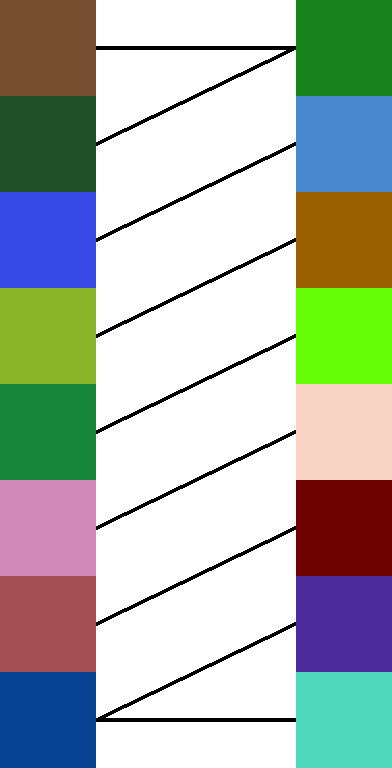
\includegraphics[width=0.30\linewidth]{img/dtw_ex2.png}
    \caption{Zuordnung der Pixel beim DTW-Algorithmus}
    \label{fig-dtw-ex2}
\end{figure}
Wie zu sehen ist, ist dieses Matching auch gültig, da jedes Element mindestens einen Partner hat und sich außerdem keine Verbindungen überkreuzen.
\section{Mahalanobis Gradient Compatibility (MGC)}\label{section-mgc}
Die Mahalanobis Gradient Compatibility (MGC) wurde zuerst in \cite{gallagher} beschrieben und später in weiteren Werken \cite{linear,paikin,loop,robust,crisjim} verwendet oder je nach Problemstellung leicht angepasst.

Bei dieser Art der Kompatibilität wird zunächst von allen vier Seiten jedes Puzzlestückes der durchschnittliche Wert der Ableitungen (vgl. \ref{section-pbc}) berechnet (für allen drei Farb-Channels). Mit diesen Ableitungen und dem Durchschnitt lässt sich dann die Kovarianzmatrix bezüglich diesen Ableitungen berechnen. Beim Vergleich zweier Puzzlestücke werden dann wieder beide Seiten betrachtet. Es wird zunächst die Mahalanobis-Distanz von allen Ableitungen zwischen den Puzzlestücken bezüglich der Verteilung von einem Puzzlestück berechnet und aufsummiert. Um die Symmetrie beizubehalten wird dies auch noch von der anderen Seite gemacht. Die Mahalanobis-Distanz berechnet dabei die (euklidische) Distanz eines Ableitungsvektors (mit drei Komponenten für die entsprechenden Channels) bezüglich eines Koordinatensystems welches durch den Durchschnittsvektor und der Kovarianzmatrix (des jeweils anderen Puzzlestückes) beschrieben wird. Der Durchschnittsvektor bildet dabei den Ursprung des Koordinatensystems und die (normierten) Eigenvektoren der Kovarianzmatrix bilden die Achsen. Die Mahalanobis-Distanz führt zunächst diese Koordinatentransformation durch, um danach die Distanz eines Vektors in diesem Koordinatensystem berechnen zu können.

Es werden im Folgenden wieder zwei Puzzlestücke $x_i$ und $x_j$ betrachtet, wobei $r=0$ und $x_i$ damit links von $x_j$ platziert wird. Die Distanz $D(x_i,x_j,r)$ wird wieder in zwei Teile aufgeteilt (ähnlich wie bei der PBC in \ref{section-pbc}): $D(x_i,x_j,r)=D_L(x_i,x_j,r)+D_R(x_i,x_j,r)$. Damit ist die Symmetrie der Distanz garantiert und es gilt $D(x_i,x_j,r)=D(x_i,x_j,r')$. Es wird im Folgenden dann nur die Berechnung für $D_L(x_i,x_j,0)$ aufgeführt. Für diese Berechnung ist es zunächst nötig, die Ableitungen von $x_i$ an der rechten Seite zu berechnen. Wie in \ref{section-pbc} wird dafür der Backward-Differenzenquotient entlang der x-Achse genommen. In der Literatur werden diese Ableitungen als Gradient $G$ bezeichnet. Für die rechte Seite von $x_i$ ergeben sich die Ableitungsvektoren dann folgendermaßen (es ist zu beachten, dass ein $G$ drei Komponenten hat):
\begin{align}\label{eq-mgc1}
    G_k=x_i(w-1,k)-x_i(w-2,k),\;\forall 0\leq k<h
\end{align}
Damit lässt sich dann der durchschnittliche Ableitungsvektor bestimmen:
\begin{align}\label{eq-mgc2}
    \mu=\frac{1}{h}\sum_{k=0}^{h-1}G_k
\end{align}
Mit allen Ableitungsvektoren und dem durchschnittlichen Ableitungsvektor lässt sich dann die Kovarianzmatrix $S$ bestimmen. Dies ist hier eine $3\times3$ Matrix und lässt sich folgendermaßen bestimmen:
\begin{align}\label{eq-mgc3}
    S=\frac{1}{h-1}\sum_{k=0}^{h-1}(G_k-\mu)(G_k-\mu)^\mathsf{T}
\end{align}
Um numerische Probleme bei der späteren Invertierung von $S$ zu vermeiden, lassen sich einige \textit{dummy} Gradienten mit in die Berechnung der Matrix $S$ einbeziehen. Dabei wurde sich an \cite{gallagher,crisjim} orientiert und es wurden neun solcher Gradienten gewählt. Diese Gradienten lauten
\begin{align*}
    &(0,0,0),(1,1,1),(-1,-1,-1),\\
    &(0,0,1),(0,1,0),(1,0,0),\\
    &(-1,0,0),(0,-1,0),(0,0,-1)
\end{align*}
Die Mahalanobis-Distanz von einem Vektor $x$ berechnet sich dann zu:
\begin{align}\label{eq-mgc4}
    D_M(x)=\sqrt{(x-\mu)^\mathsf{T}S^{-1}(x-\mu)}
\end{align}
Es ist nun möglich mit \ref{eq-mgc2}, \ref{eq-mgc3} und \ref{eq-mgc4} die einseitige Gesamtdistanz $D_L(x_i,x_j,0)$ zu definieren. Dabei ist lediglich zu beachten, dass nach \cite{gallagher} die Wurzeloperation aus \ref{eq-mgc4} weggelassen wird.
\begin{align}\label{eq-mgc5}
    D_L(x_i,x_j,0)=\sum_{k=0}^{h-1}(G_k^{i\rightarrow j}-\mu)^\mathsf{T}S^{-1}(G_k^{i\rightarrow j}-\mu)
\end{align}
Dabei ist $G_k^{i\rightarrow j}$ der Ableitungsvektor der beim Übergang von einem Puzzlestück zum anderen entsteht, wenn man die beiden Puzzlestücke $x_i$ und $x_j$ nun (mit $x_i$ links von $x_j$) zusammenfügt. Dafür gilt:
\begin{align}\label{eq-mgc6}
    G_k^{i\rightarrow j}=x_j(0,k)-x_i(w-1,k),\;\forall 0\leq k<h
\end{align}
Bezüglich der Implementation lässt sich sagen, dass es durchaus möglich ist (ähnlich wie in \ref{section-pbc}), die Ableitungsvektoren, den durchschnittlichen Ableitungsvektor und auch die Inverse der Kovarianzmatrix (es wird zu jederzeit nur die Inverse von $S$ benötigt, daher lohnt es sich nicht auch $S$ selber abzuspeichern) jeder Seite (und für jedes Puzzlestück) nur einmal zu berechnen und diese dann abzuspeichern. Bei dem eigentlichen Vergleich zweier Puzzlestücke müssen dann nur \ref{eq-mgc5} und \ref{eq-mgc6} berechnet werden. Trotz der großen Anzahl und höheren Komplexität der Berechnungen, ist das Laufzeitverhalten der kompletten Prozedur linear in der Länge der Kante (beispielsweise $h$ wie in den obigen Gleichungen). Berechnungen wie \ref{eq-mgc3} oder \ref{eq-mgc5} haben aufgrund der Matrizenmultiplikationen zwar größeren konstanten Aufwand (in der Summe), da jede Matrix aber die Dimensionen $1\times3$, $3\times1$ oder $3\times3$ besitzt, sind die Dimensionen der Matrizen und somit auch alle Operationen mit diesen Matrizen konstant.

Diese Linearität dieses Verfahrens bietet einen großen Vorteil bei der Berechnung von sehr hochauflösenden Bildern (bzw. hochauflösenden Puzzlestücken). Verfahren wie etwa DTW (\ref{section-dtw}) sind dort aufgrund der quadratischen Laufzeit eher weniger geeignet. Diese Tatsache und ein komplexeres Verfahren zur Bewertung der Übergänge zwischen zwei Puzzlestücken (im Vergleich zu der trivialeren PBC in \ref{section-pbc}), hat dazu geführt, dass selbst komplexere Jigsaw-Puzzle-Solver (wie etwa \cite{paikin}) noch diese Metrik verwenden. Aus diesen Gründen wurde diese Metrik auch für den folgenden Algorithmus verwendet.
\chapter{Algorithmus zur Puzzle-Assemblierung}
Ausgestattet mit einer Vielzahl von Metriken aus \ref{ch-metrics} gilt es nun einen Algorithmus zu entwickeln, der die eigentliche Assemblierung des Puzzles übernimmt. Dabei wird aktuell noch von einem Jigsaw-Puzzle ausgegangen bei dem keine Puzzlestücke fehlen (bei Schiebepuzzles fehlt entsprechend ein Stück, auf diesen Sonderfall wird dort eingegangen, wo dieser Fall Probleme beim Algorithmus bereitet). Da das Jigsaw-Puzzle nachweisbar als NP-Hard gilt \cite{dem}, beruhen alle bekannten algorithmischen Puzzle-Löser auf einen heuristischen Ansatz, um große Puzzle lösen zu können.

Aktuelle Methoden zum Lösen von Jigsaw-Puzzles lassen sich grob in zwei Kategorien aufteilen:
\begin{enumerate}
    \item Greedy Methoden \cite{loop,pomeranz,gallagher}, welche probieren aus den paarweisen Distanzen der einzelnen Puzzlestücke iterativ ein Gesamtbild zu assemblieren, indem in jedem Schritt die günstigsten bzw. besten Puzzlestücke miteinander verbunden werden.
    \item Globale Methoden, welche probieren eine globale Kompatibilitätsfunktion zu maximieren (bzw. eine globale Distanzfunktion zu minimieren) um dabei ein globales Maximum (oder Minimum im Falle einer Distanzfunktion) zu finden. Darunter fallen unter anderem Ansätze aus der genetischen Programmierung \cite{genetic}, linearen Programmierung \cite{linear} und auch probabilistische Verfahren \cite{cho}.
\end{enumerate}
In dieser Arbeit wird sich auf das Spannbaum Verfahren von Gallagher \cite{gallagher} fokussiert. Dieses Verfahren lässt sich in die Kategorie der Greedy Methoden einordnen und basiert hauptsächlich auf der Observierung, dass gängige Algorithmen zur Berechnung eines minimalen Spannbaums (Minimum Spanning Tree - MST) mit wenigen Änderungen bereits in der Lage dazu sind, simple Jigsaw-Puzzle zu assemblieren. Diese Idee wurde dann so perfektioniert, dass Gallagher selber in der Lage dazu war, Puzzle mit mehreren tausend Puzzlestücken perfekt zu rekonstruieren. Neben dieser vielversprechenden Ergebnisse und der Tatsache, dass dieses Verfahren auch das erste Verfahren war, welches die MGC (vgl. \ref{section-mgc}) verwendet hat (auch diese wurde von Gallagher selber in \cite{gallagher} beschrieben), basiert dieses Verfahren trotz State-of-the-Art Ergebnisse hauptsächlich auf Methoden der Graphentheorie. Andere Verfahren mit vergleichbaren Ergebnissen (etwa das probabilistische Verfahren von Cho et al. \cite{cho}) basieren auf tiefliegendere und komplexere stochastische Zusammenhänge.

Neben dem Algorithmus selber und einige Änderungen um diesen auch für Schiebepuzzle möglich zu machen, wird außerdem eine effiziente Datenstruktur beschrieben, auf die der Algorithmus arbeiten wird. Dabei handelt es sich um eine modifizierte Version der Disjoint-Set-Datenstruktur oder auch Disjoint-Set-Forest.\cite{dsf} Bei den Anforderungen dieser Datenstruktur wird sich sowohl an Gallagher selber gerichtet \cite{gallagher}, als auch an C. Zanoci und J. Andress Beschreibung von Gallaghers Algorithmus.\cite{crisjim}
\section{Baum-basierte Assemblierung nach Gallagher}
Es wird das Jigsaw-Puzzle Problem als Graph $G=(V,E)$ betrachtet mit der Menge der Puzzlestücke als Vertices $V$ und die Menge der möglichen Verbindungen von zwei Puzzlestücken als Kanten $E$. Diese Kanten sind gewichtet und erhalten ihre Kantengewichte nach einer der in Kapitel \ref{ch-metrics} vorgestellten Metriken (vorzugsweise die MGC). Außerdem sei zu beachten, dass zwei Puzzlestücken nicht nur durch eine Kante sondern durch exakt vier Kanten in Verbindung stehen - jeweils eine für jede mögliche räumliche Anordnung der beiden Puzzleteile (vgl. Tabelle \ref{tbl-spatial-relation}).

Da das fertige Puzzle eine Zusammenhangskomponente des Graphen darstellt (und zwar eine mit minimaler oder nahezu minimaler Kantengewichtssumme), bietet sich ein Algorithmus zur Berechnung des minimalen Spannbaums an. Ein solcher Algorithmus wäre in der Lage eine solche minimale Zusammenhangskomponente zu finden. Der minimale Spannbaum der durch einen solchen Algorithmus entstehen würde stellt in aller Regel jedoch keine legale Puzzlestellung dar. Dazu muss zusätzlich noch sichergestellt werden, dass jederzeit keine zwei Puzzlestücke in der Zusammenhangskomponente übereinander liegen. Diese zusätzliche Einschränkung des Algorithmus ist eine weitere Motivation für die Implementation einer modifizierten Disjoint-Set-Datenstruktur, die den räumlichen Zusammenhang der Zusammenhangskomponenten kennt und vermeidet, dass Zusammenhangskomponenten zusammengeführt werden, welche zu übereinander liegenden Puzzlestücken führen würden.

Entsprechend solch einer Datenstruktur wird damit im Zusammenhang der Algorithmus von Kruskal \cite{kruskal} betrachtet, um den minimalen Spannbaum in einem Graphen zu finden. Dabei werden am Anfang des Algorithmus alle Vertices (die Puzzlestücke) zunächst als seperate Zusammenhangskomponenten aufgefasst. Damit bildet jeder Vertex einen Baum, die Menge aller Bäume wird als Wald (Forest) bezeichnet. Daraufhin werden die Kanten des Graphen in absteigender Reihenfolge (bezüglich des Kantengewichts) betrachtet. Verbindet eine Kante zwei Vertices, welche sich bereits in der selben Zusammenhangskomponente befinden, so wird diese Kante nicht zum Baum hinzugefügt, da diese dort sonst eine Schleife erzeugen würde. Im Falle wo diese Kante zwei Vertices verbinden würde, welche sich in verschiedenen Zusammenhangskomponenten befinden, so wird diese Kante zum Baum hinzugefügt. Dieser Schritt verbindet die beiden Zusammenhangskomponenten zu einer größeren Zusammenhangskomponente. Dieser Vorgang wird solange wiederholt, wie noch Kanten vorhanden sind und es sich noch kein Spannbaum gebildet hat (es existieren noch mindestens zwei seperate Bäume im Wald).

Die normale Disjoint-Set-Datenstruktur (Disjoint-Set-Forest) \cite{dsf} übernimmt dabei die Aufgabe, die Menge der Vertices $V$ in disjunkte zusammenhängende Mengen (Zusammenhangskomponenten) zu partitionieren. Die üblichen Operationen auf eine solche Datenstruktur sind unter anderem das Initialisieren eines solchen disjunkten Waldes mit $n$ Elementen (was in $\Theta(n)$ Zeit möglich ist), das Testen, ob zwei Elemente sich in der selben Menge befinden und das Vereinigen zweier Mengen.

Die Laufzeit der letzten beiden Operationen hängt stark von der Implementation der Datenstruktur ab. Bei einer guten Implementation sind beide Operationen durchschnittlich $\Theta(\alpha(n))$.\cite{dsf-log,dsf-lower,tarjan,tarjan2,tarjan3} Wobei $\alpha(n)$ für die inverse Funktion der eindimensionalen Ackermann-Funktion $f(n)=A(n,n)$ steht. Die Funktion $f(n)$ nimmt bereits für kleine $n$ sehr große Werte an. So ist bereits $f(4)=A(4,4)=2\uparrow\uparrow7-3$ in Knuth's \textit{uparrow} Notation. Als Potenz ergibt sich der \textit{Power-Tower} $f(4)=2^{2^{2^{2^{2^{2^2}}}}}-3$. Die einfachste Potenz die dies noch darstellen kann ist $f(4)=2^{2^{2^{65536}}}-3$. Selbst die innerste Potenz $2^{65536}$ ist bereits unvorstellbar groß. Dementsprechend lässt sich sagen, dass die inverse Ackermann-Funktion selbst für sehr große $n$ stets Werte annehmen wird, die $4$ nicht überschreiten. Damit lässt sich sagen, dass Operationen mit einem Laufzeitverhalten von $\Theta(\alpha(n))$ \textit{quasi konstant} sind.

Ein Disjoint-Set-Forest (DSF) wird in der Regel als kompaktes Array implementiert. Jedes Element im Array ist dann ein Element im Forest (also ein Element eines Baums im Wald). Die Array-Indizes können dann dazu dienen die Elemente zu identifizieren. Jedes Element enthält dann zusätzlich noch einen Parent-Pointer (bei Arrays bietet sich auch ein Parent-Index an). Um zwei Mengen später effizient vereinigen zu können, lässt sich auch noch ein zusätzliches Feld definieren, welches die Anzahl der Elemente mitspeichert, die sich in dem selben Baum wie das Element befinden. Dieses Feld ist nur für Elemente von Bedeutung, die die Wurzel ihres Baumes darstellen (da nur dort die Anzahl erhöht wird). Die Beziehungen der Elemente über den Parent-Index bilden einen \textit{rückverweisenden} Baum: Es lässt sich bei jedem beliebigen Element starten und solange der Parent-Index verfolgen, bis dieser entweder ungültig (\texttt{null}) ist oder (bei Arrays üblich) ein Element der Parent von sich selber ist. Dieses Element ist die Wurzel des Baums, der alle Elemente enthält, die dieses Element auch als Wurzel haben. Dieses Wurzelelement \textit{repräsentiert} seine Menge.

Die \texttt{InitForest} Operation initialisiert einen DSF mit einer vorgegeben Kapazität $n$. Jedes Element befindet sich anfangs in seiner eigenen Menge.
\begin{algorithm}[H]
    \caption{Initialisierung eines Disjoint-Set-Forest}\label{alg-dsf-init}
    \begin{algorithmic}
        \Procedure{InitForest}{$n$}
            \State nodes $\gets$ array$[n]$
            \For{$i=1$ to $n$}
                \State nodes$[i]$.parent $\gets i$\Comment{Element ist Wurzel seiner Menge}
                \State nodes$[i]$.size $\gets 1$\Comment{Menge enthält nur dieses Element}
            \EndFor
        \EndProcedure
    \end{algorithmic}
\end{algorithm}
Die \texttt{FindRoot} Operation übernimmt den Index $i$ eines Elementes $x_i$ und gibt den Index des Wurzelelementes der Menge zurück in der sich $x_i$ befindet. Diese Operation arbeitet sich solange den Baum hoch bis ein Element gefunden wurde, welches als Parent-Index sich selbst eingetragen hat. Der Index dieses Elementes wird dann zurückgegeben. An dieser Stelle lässt sich noch eine wichtige Verbesserung vornehmen, welche notwendig (jedoch noch nicht hinreichend) dafür ist, das durch die inverse Ackermann-Funktion beschränkte Laufzeitverhalten zu garantieren. Diese Erweiterung wird als Pfadkomprimierung bezeichnet und soll dafür sorgen, dass alle Elemente die auf dem Weg der \texttt{FindRoot} Operation betrachtet werden, als direkte Kinder des Wurzelelementes eingetragen werden. Damit wird ein gegebenenfalls sehr langer Pfad im Baum durch viele kleine Pfade (direkte Verbindungen zwischen den Elementen des Pfades und des Wurzelelementes) ersetzt. Dies ist eine valide Operation, da die Zugehörigkeit zu einer Menge lediglich von dem Wurzelelement des Baums bestimmt wird und in keinster Weise von den Beziehungen abhängt, die die Elemente untereinander haben. Dadurch das Bäume so stets \textit{flach} gehalten werden, wird das Laufzeitverhalten dieser und anderer Operationen die den Baum nach oben traversieren deutlich verbessert. Die \texttt{FindRoot} Operation mit Pfadkomprimierung wird dann in der Regel folgendermaßen rekursiv definiert:
\begin{algorithm}[H]
    \caption{FindRoot Operation mit Pfadkomprimierung}\label{alg-dsf-find}
    \begin{algorithmic}
        \Function{FindRoot}{$i$}
            \If{nodes$[i]$.parent $\neq i$}
                \State nodes$[i]$.parent $\gets$ FindRoot(nodes$[i]$.parent)
            \EndIf
            \State \Return nodes$[i]$.parent
        \EndFunction
    \end{algorithmic}
\end{algorithm}
Die \texttt{Union} Operation übernimmt zwei Indizes $i,j$, welche für die Elemente $x_i,x_j$ stehen und vereinigt die Menge in der sich $x_i$ befindet mit der Menge in der sich $x_j$ befindet. Falls $x_i$ und $x_j$ sich bereits in der selben Menge befinden, muss die Operationen keine weiteren Änderungen an der Datenstruktur vornehmen. Ein Wahrheitswert als Rückgabewert der Funktion informiert darüber, ob die Mengen vereinigt wurden (\texttt{true}) oder nicht (\texttt{false}). Der Algorithmus bestimmt dafür zunächst die beiden Indizes $k,l$ der Wurzelelemente $r_i,r_j$ indem die Operation \texttt{FindRoot} entsprechend mit $i$ und $j$ aufgerufen wird. Sind diese Indizes gleich so wird \texttt{false} zurückgegeben. Andernfalls wird eines der beiden Wurzelelemente (hier beispielsweise $r_j$) als das neue Wurzelelement für die vereinigte Menge festgelegt. Dafür wird der Parent von $r_i$ auf den Index von $r_j$ gesetzt. Ein kompletter Baum wird also direkt an der Wurzel des anderen Baumes angehängt. Es entsteht ein neuer großer Baum. Selbst mit Pfadkomprimierung in der \texttt{FindRoot} Operation kann das Vereinigen zweier Mengen dazu führen, dass die Bäume sehr schnell in die Tiefe wachsen (wodurch die \texttt{FindRoot} Operation und damit auch die \texttt{Union} Operation lange Pfade traversieren muss). Als weitere notwendige Erweiterung für die Effizient der Datenstruktur (entsprechend der inversen Ackermann-Funktion) muss versichert werden, dass stets der kleinere der beiden Bäume an den größeren angehängt wird. Dabei bezieht sich die Größe der Bäume auf die Anzahl der Elemente in der Menge. Diese Erweiterung wird als \textit{Union by Size} bezeichnet. Zusammen mit der Pfadkomprimierung in \texttt{FindRoot} ist damit das durchschnittliche Laufzeitverhalten von $\Theta(\alpha(n))$ garantiert.
\begin{algorithm}[H]
    \caption{Union Operation als Union by Size}\label{alg-dsf-union}
    \begin{algorithmic}
        \Function{Union}{$i,j$}
            \State $k\gets$ FindRoot(i)
            \State $l\gets$ FindRoot(j)
            \If{$k=l$}
                \State \Return false\Comment{$x_i$ und $x_j$ befinden sich in der selben Menge}
            \EndIf
            \If{nodes$[k]$.size $>$ nodes$[l]$.size}
                \State Swap($k,l$)\Comment{$k$ ist der Wurzelindex der kleineren Menge}
            \EndIf
            \State nodes$[k]$.parent $\gets l$\Comment{Kleinere Menge an die größere anhängen}
            \State nodes$[l]$.size $\gets$ nodes$[l]$.size $+$ nodes$[k]$.size\Comment{Anzahl aktualisieren}
            \State \Return true
        \EndFunction
    \end{algorithmic}
\end{algorithm}
Um die normale DSF-Datenstruktur für das rekonstruieren von Puzzles anzupassen, müssen zunächst weitere Attribute zu der Datenstruktur hinzugefügt werden, welche die räumliche Beziehung der Mengenelemente (welche jetzt konkret Puzzlestücke sind) beschreiben.

Neben einem Parent-Index, sollte jedes Element zusätzlich noch seine relative Position zu seinem Parent in Form von zweidimensionalen Koordinaten abspeichern. Dabei zeigt die positive x-Achse wieder nach rechts und die positive y-Achse nach unten. Die Koordinaten eines Elementes $v$ bezüglich seines Parent $p$ wird dann durch den Vektor von $p$ nach $v$ ausgedrückt: $\vv{pv}$. Alle Elemente einer Menge befinden sich in einem gemeinsamen Koordinatensystem, wobei das Wurzelelement den Ursprung dieses Koordinatensystems bildet.

Auch das Attribut welches die Anzahl der Elemente in der Menge des Elementes angibt (welches lediglich dann von Nutzen ist, wenn das Element ein Wurzelelement ist) lässt sich ersetzen (dabei muss aufgepasst werden, dass diese Information nicht komplett verloren geht, da die Anzahl für Algorithmus \ref{alg-dsf-union} benötigt wird). Stattdessen bekommt jedes Element (auch wenn das Attribut wieder nur für Wurzelelemente gedacht ist) eine Menge von geordneten Paaren. Diese Paare bestehen aus einem Elementindex und aus einer Koordinate. Ein solches Paar repräsentiert ein Element $v$ im Baum des Wurzelelementes $r$ und die Koordinate ist die \textit{absolute} Koordinate dieses Elementes im Koordinatensystem der Menge (also $\vv{rv}$). Jedes Wurzelelement kennt also alle Elemente seiner Menge und weiß auch wo diese Elemente sich relativ zu ihm befinden. Die Kardinalität der Menge ist dann die Anzahl der Elemente in diesem Baum, womit klar wird wieso das Attribut \texttt{size} entfernt wurde: Diese Information ist nun implizit durch die Menge aller Elemente gegeben.

Als letztes Attribut soll sich die Datenstruktur auch merken, wie viele aktive Bäume sich im Wald befinden. Anfangs sind dies $n$ Bäume für $n$ Elemente (da jedes Element in seiner eigenen Menge ist), im Hinblick auf den Algorithmus von Kruskal ist es aber besonders interessant, wann diese Anzahl $1$ ist (und somit eine Zusammenhangskomponente entstanden ist).

Damit lassen sich nun Algorithmen \ref{alg-dsf-init}, \ref{alg-dsf-find}, \ref{alg-dsf-union} so anpassen, dass die Datenstruktur für die Rekonstruktion von Puzzles geeignet ist (und somit die Aufgabe übernimmt, nur gültige Zusammensetzungen von Puzzlestücken als Zusammenhangskomponenten zuzulassen).
\begin{algorithm}[H]
    \caption{Erweiterte InitForest Operation}\label{alg-dsf-init2}
    \begin{algorithmic}[1]
        \Procedure{InitForest}{$n$}
            \State nodes $\gets$ array$[n]$
            \State tree\_count $\gets n$\Comment{Anzahl der aktiven Bäume ist anfangs $n$}
            \For{$i=1$ to $n$}
                \State nodes$[i]$.parent $\gets i$\Comment{Element ist Wurzel seiner Menge}
                \State nodes$[i]$.parent\_coords $\gets(0,0)$
                \State nodes$[i]$.tree $\gets$ set$\{(index:i,root\_coords:(0,0))\}$
            \EndFor
        \EndProcedure
    \end{algorithmic}
\end{algorithm}
Zeile 6 in Algorithmus \ref{alg-dsf-init2} definiert für ein Element $v$ die relativen Koordinaten zu seinem Parent als die Koordinaten des Vektors $\vv{pv}$. Da alle Elemente aber anfangs sich selber als Parent haben gilt $\vv{pv}=\vv{vv}=\vec{0}$. Zeile 7 erstellt die Menge, die alle Elemente mit Index und Koordinate (bezüglich des Wurzelelement der Menge) enthält. Anfangs ist jedes Element in seiner eigenen Menge und das einzige Paar was bei der Initialisierung eingetragen werden muss ist das mit Paar mit dem Index des eigenen Elementes und den Koordinaten $(0,0)$. Da jedes Element anfangs die Wurzel seiner Menge darstellt, befindet sich dieses Element auch im Ursprung des Koordinatensystems (welches ja seinen Ursprung beim Wurzelelement der Menge hat). Anders gesagt ist anfangs $r=v$ und damit $\vv{rv}=\vv{vv}=\vec{0}$.
\begin{algorithm}[H]
    \caption{Erweiterte FindRoot Operation}\label{alg-dsf-find2}
    \begin{algorithmic}[1]
        \Function{FindRoot}{$i$}
            \If{nodes$[i]$.parent $\neq i$}
                \State k $\gets$ FindRoot(nodes$[i]$.parent)
                \State $\vv{rp}\gets$ nodes$[$nodes$[i]$.parent$]$.parent\_coords
                \State nodes$[i]$.parent\_coords $\gets\vv{rp}$ $+$ nodes$[i]$.parent\_coords
                \State nodes$[i]$.parent = k
            \EndIf
            \State \Return nodes$[i]$.parent
        \EndFunction
    \end{algorithmic}
\end{algorithm}
Algorithmus \ref{alg-dsf-find2} übernimmt neben der Rückgabe des Wurzelindex weiterhin eine Pfadkomprimierung. Da die Koordinaten eines Elementes $v$ bezüglich seines Parent $p$ bei der Pfadkomprimierung ihre Gültigkeit verlieren, weil das Element durch die Komprimierung einen neuen Parent (das Wurzelelement) bekommt, muss die Koordinate von $\vv{pv}$ auf $\vv{rv}$ geändert werden. Dazu muss jedoch zunächst $\vv{rp}$ bekannt sein. Diesen Vektor bekommt man durch einen rekursiven Aufruf von \texttt{FindRoot} mit dem Parent als Parameter. Dann wird dort die Pfadkomprimierung angestoßen und $p$ bekommt die Wurzel als Parent. Dies geht bis zum Basisfall der Rekursion weiter. Beim Abbau der Rekursion werden dann alle Vektoren aufaddiert. Für einen Pfad von $v$ nach $r$ mit $m$ Zwischenelementen $q_1\dots q_m$ baut sich durch die Rekursion folgende Summe auf:$$\underbrace{\vec{0}+\vv{r q_m}+\vv{q_m q_{m-1}}+\dots+\vv{q_2 q_1}}_{\vv{r q_1}}+\vv{q_1 v}=\vv{r v}$$
Damit lässt sich erklären, was genau in Algorithmus \ref{alg-dsf-find2} passiert (und warum die Reihenfolge der einzelnen Statements genau so gewählt ist). Beim Aufruf von \texttt{FindRoot} mit einem Index der für Element $v$ steht, wird in Zeile 3 der Index des Wurzelelementes zwischengespeichert ($k$). Viel wichtiger noch ist, dass nach Abschluss dieser Zeile der rekursive Schritt fertig ist und für das Parent-Element $p$ nun im Koordinaten-Feld der Vektor $\vv{rp}$ steht. Da der Index des Parents noch bekannt ist (deswegen wurde der Index des Wurzelelementes zunächst nur zwischengespeichert), lässt sich dieser Vektor einfach nach Zeile 4 auslesen. Die Addition in Zeile 5 berechnet dann $\vv{rp}+\vv{pv}=\vv{rv}$. Jetzt lässt sich ohne Probleme die Pfadkomprimierung abschließen, indem man das zuvor gefundene Wurzelelement als Parent von $v$ erklärt (Zeile 6).

Als simples Beispiel ist in Abbildung \ref{fig-dsf-vec} ein Koordinatensystem dargestellt. Es wird ein Element $v$ betrachtet mit einem Parent $p$, Grandparent $g$ und Root $r$. Dabei ist $r$ der Ursprung des Koordinatensystems. Die Vektoren $\vv{pv},\vv{gp},\vv{rg}$ beschreiben die relativen Position von einem Element bezüglich seines Parents. Ziel ist es $\vv{rv}=\vv{rg}+\vv{gp}+\vv{pv}$ zu berechnen. Die Rekursion bewirkt, dass zunächst $\vv{rp}=\vv{rg}+\vv{gp}$ berechnet wird und dann mit dem Ergebnis das gesuchte $\vv{rv}=\vv{rp}+\vv{pv}$.
\begin{figure}[H]
    \centering
    \begin{tikzpicture}
        \draw[step=1cm,gray,very thin] (0,0) grid (8,8);
        
        \draw[thick] (0.5,4)--(4,4);
        \draw[thick] (4,7.5)--(4,4);
        \draw[thick,->] (4,4) node[anchor=south east] {$r$} -- (7.5,4) node[anchor=west] {$x$};
        \draw[thick,->] (4,4) -- (4,0.5) node[anchor=north] {$y$};

        \fill[black] (6,1) node[anchor=north west] {$v$} circle (0.04cm);
        \fill[black] (2,2) node[anchor=north east] {$p$} circle (0.04cm);
        \fill[black] (7,5) node[anchor=south west] {$g$} circle (0.04cm);

        \draw[red,thick,->] (4,4) -- (6.98,4.98) node[above,midway] {$\vv{rg}$};
        \draw[blue,thick,->] (7,5) -- (2.02,2.02) node[below,pos=0.40] {$\vv{gp}$};
        \draw[purple,thick,->] (2,2) -- (5.98,1.02) node[below,midway] {$\vv{pv}$};
        \draw[black!40!green,thick,->] (4,4) -- (2.02,2.02) node[above,pos=0.60] {$\vv{rp}=\vv{rg}+\vv{gp}$};
        \draw[orange,thick,->] (4,4) -- (5.98,1.02) node[above,midway] {$\;\;\;\;\;\;\;\;\;\;\;\;\;\;\;\;\;\;\;\;\;\;\;\;\;\;\vv{rv}=\vv{rg}+\vv{gp}+\vv{pv}=\vv{rp}+\vv{pv}$};
    \end{tikzpicture}
    \caption{Koordinatentransformation im DSF bei Pfadkomprimierung}
    \label{fig-dsf-vec}
\end{figure}
Bei der \texttt{Union} Operation gilt es nun die neuen implementierten Informationen (in Form von räumlichen Beziehungen der Elemente) so zu verwenden, dass nur dann vereinigt wird, wenn dabei keine zwei Puzzlestücke übereinander liegen. Dazu wird optimistischer Weise eine Vereinigung der beiden Mengen berechnet, welche die Paare von Elementindizes inklusive Koordinaten enthalten. Da diese Koordinaten sich jedoch auf zwei verschiedene Koordinatensysteme beziehen, muss zunächst in einer dieser Mengen eine Transformationen dieser Koordinaten vorgenommen werden. Diese Vereinigung wird dann nur bezüglich der Koordinate eines solchen Paares gebildet. Mit der Kardinalität dieser Vereinigungsmenge lässt sich dann feststellen, ob die beiden Bäume vereinigt werden können oder nicht. Da nun das Vereinigen zweier Bäume konkret das Zusammenstecken zweier Puzzlestücke darstellt ist es bei dieser Operation nun auch notwendig zu wissen, wie diese beiden Stücke zusammengesetzt werden. Dazu wird eine numerische Konstante $r$ definiert nach Tabelle \ref{tbl-spatial-relation} mit übergeben.
\begin{algorithm}[H]
    \caption{Erweiterte Union Operation}\label{alg-dsf-union2}
    \begin{algorithmic}[1]
        \Function{Union}{$i,j,r$}
            \State $k\gets$ FindRoot(i)
            \State $l\gets$ FindRoot(j)
            \If{$k=l$}
                \State \Return false\Comment{$v_i$ und $v_j$ befinden sich in der selben Menge}
            \EndIf
            \If{nodes$[k]$.tree.size $>$ nodes$[l]$.tree.size}
                \State Swap($k,l$)\Comment{$k$ ist der Wurzelindex der kleineren Menge}
                \State Swap($i,j$)\Comment{$i$ ist Index vom Element der kleineren Menge}
                \State $r\gets(r+2)\bmod4$\Comment{Inverse Beziehung von $v_i,v_j$ berechnen}
            \EndIf
            \State tree$_i^\prime$ $\gets$ set $\{\}$
            \ForAll{$(u,\vv{r_i v_u})\in$ nodes$[k]$.tree}
                \State tree$_i^\prime$ $\gets$ tree$_i^\prime$ $\cup\:\{(u,\vv{r_j r_i}+\vv{r_i v_u})\}$
            \EndFor
            \If{tree$_i^\prime$ $\cap$ nodes$[l]$.tree $\neq\varnothing$}
                \State \Return false\Comment{Stücke überschneiden sich}
            \EndIf
            \State nodes$[l]$.tree $\gets$ nodes$[l]$.tree $\cup$ tree$_i^\prime$
            \State nodes$[k]$.parent $\gets l$\Comment{Kleinere Menge an die größere anhängen}
            \State nodes$[k]$.parent\_coords $\gets\vv{r_j r_i}$
            \State nodes$[k]$.tree $\gets$ set $\{\}$
            \State tree\_count $\gets$ tree\_count $-\:1$
            \State \Return true
        \EndFunction
    \end{algorithmic}
\end{algorithm}
Der interessante Teil des Algorithmus läuft zwischen Zeile 12 und 19 ab. Kommt der Algorithmus erfolgreich bis Zeile 12, so befinden sich die beiden Elemente $v_i,v_j$ nicht in der selben Menge. Außerdem ist an dieser Stelle sichergestellt, dass $v_i$ stets das Element der kleineren Menge ist (die Wurzel $r_i$ des Baumes dieses Elementes soll an die Wurzel $r_j$ des größeren Baumes des anderen Elementes angehängt werden). Beide Wurzeln $r_i,r_j$ kennen alle Elemente ihrer Menge mit den Koordinaten in dem Koordinatensystem der Menge. Beim Vereinigen bekommt $r_j$ nun alle Elemente von $r_i$. Dazu müssen aber die Koordinaten aller Elemente zunächst angepasst werden. Für ein Element $v_u$ in der Menge von $r_i$ ist die Koordinate dieses Elementes in der Form $\vv{r_i v_u}$ angegeben. Um $v_u$ in die Menge aller Elemente aus $r_j$ übernehmen zu können muss diese Koordinate in die Form $\vv{r_j v_u}$ gebracht werden. Dazu muss berechnet werden:
\begin{align}\label{eq-dsf-trans}
    \vv{r_j v_u}&=\vv{r_j r_i}+\vv{r_i v_u}
\end{align}
Es ist also der Vektor $\vv{r_j r_i}$ gesucht (die relative Position von der Wurzel $r_i$ zu $r_j$). Diese standen zuvor in keinerlei Beziehung, da jede Menge ihr eigenes Koordinatensystem besitzt. Bei der Zusammensetzung von $v_i$ und $v_j$ lässt sich jedoch eine Beziehung der beiden Wurzeln beschreiben. Zunächst sei gesagt, dass der Parameter $r$ der Methode (die räumliche Beziehung der beiden Elemente) exakt den Vektor $\vv{v_j v_i}$ bestimmt. Dieser lässt sich direkt der Tabelle \ref{tbl-spatial-relation} entnehmen. Beispielsweise ist $\vv{v_j v_i}=(-1,0)$ genau dann wenn $r=0$.

Da beide Wurzeln alle Koordinaten ihrer Elemente kennen (und somit auch die Koordinaten der entsprechenden $v$'s), könnte man diese Menge durchsuchen. Dies dauert aber zu lange und ist dank der neuen erweiterten Pfadkomprimierung aus Algorithmus \ref{alg-dsf-find2} nicht nötig. In Zeile 2 und 3 von Algorithmus \ref{alg-dsf-union2} werden die Indizes von $r_i,r_j$ bestimmt dabei werden $v_i,v_j$ aber direkte Kinder ihrer entsprechenden Wurzeln. Dank der Koordinatentransformation nach Abbildung \ref{fig-dsf-vec} stehen die Koordinaten $\vv{r_i v_i}$ und $\vv{r_j v_j}$ direkt als Attribut in den jeweiligen Elementen drin. Damit sind alle Informationen zur Berechnung von $\vv{r_j r_i}$ vollständig und es gilt:
\begin{align}\label{eq-dsf-trans2}
    \vv{r_j r_i}&=\vv{r_j v_j}+\vv{v_j v_i}+\underbrace{\vv{v_i r_i}}_{=-\vv{r_i v_i}}\nonumber\\
    \vv{r_j r_i}&=\vv{r_j v_j}+\vv{v_j v_i}-\vv{r_i v_i}
\end{align}
Somit lässt sich $\vv{r_j r_i}$ noch vor den Eintritt in die Schleife in Zeile 13 berechnen. Diese Schleife verwendet dann $\vv{r_j r_i}$ zusammen mit Gleichung \ref{eq-dsf-trans} lässt sich dann $\vv{r_j v_u}$ berechnen. Am Ende der Schleife ergibt sich die Menge aller Paare mit Elementen von $r_i$ jedoch in den Koordinaten von $r_j$. Jetzt lässt sich bezüglich der Koordinaten dieser Paare die Durchschnittsmenge von dieser neu berechneten Menge und von der Menge bilden, die $r_j$ bereits kennt. Ist diese Durchschnittsmenge nicht leer, so bekommen zwei Elemente beim Vereinigen der Bäume die gleiche Koordinate. Anders gesagt: Zwei Puzzlestücke würden sich überschneiden. Andernfalls kann bereits die Vereinigungsmenge der beiden Paar-Mengen gebildet werden, diese muss schließlich die alte Paar-Menge von $r_j$ überschreiben. In der Implementation wird oftmals wie schon erwähnt ein optimistischer Ansatz gewählt und es wird direkt die Vereinigungsmenge gebildet, da die Durchschnittsmenge eigentlich nicht gebraucht wird (außer um auf eine nicht leere Menge zu überprüfen). Nach dem Inklusion-Exklusion-Prinzips lässt sich die Kardinalität der Durchschnittsmenge dann aus den Kardinalitäten der beiden Mengen und der Kardinalität der Vereinigungsmenge berechnen: $|A\cap B|=|A|+|B|-|A\cup B|$. Diese Kardinalität lässt sich dann auf $0$ überprüfen und es muss stets nur eine Mengenoperation angewandt werden.

Das Zurücksetzen der Paar-Menge von dem (nun nicht mehr Wurzel-) Element $r_i$ in Zeile 22 ist optional, bietet sich jedoch an um den Speicheraufwand der Datenstruktur zu verringern.

Da bei der Vereinigungsoperation nur ein Element ($r_i$) seinen Parent (von keinen Parent auf $r_j$) ändert (abgesehen von der Pfadkomprimierung die implizit im Algorithmus stattfindet), gibt es auch nur eine Parent-Koordinate, welche angepasst werden muss. Dies geschieht in Zeile 21 mit dem zuvor berechneten Vektor $\vv{r_j r_i}$, welcher genau diese relative Koordinate vom Element $r_i$ relativ zu seinem neuen Parent $r_j$ beschreibt. Alle Elemente unterhalb von $r_i$ ändern zwar implizit ihr Wurzelelement von $r_i$ auf $r_j$, jedoch nicht ihr Parent-Element, womit alle Parent-Koordinaten weiterhin konsistent sind.

Damit ist der Hauptalgorithmus der Datenstruktur komplett beschrieben. An dieser Stelle sollte klar sein, dass iteratives Vereinigen der Bäume zu einer Zusammenhangskomponente führt, welche außerdem keine Puzzlestücke enthält, die sich überschneiden. Damit ist jedoch noch nicht garantiert, das das entstandende Bild auch die gewünschten Dimensionen des Puzzles ($m\times n$) besitzt. Auch dazu wird sich an Gallagher \cite{gallagher,crisjim} orientiert und noch zwei simple Schritte eingeführt: Trimming und Filling.
\begin{figure}[H]
    \centering
    \subfloat[Ausgangspuzzle\label{fig-dsf-stages-1}]{
      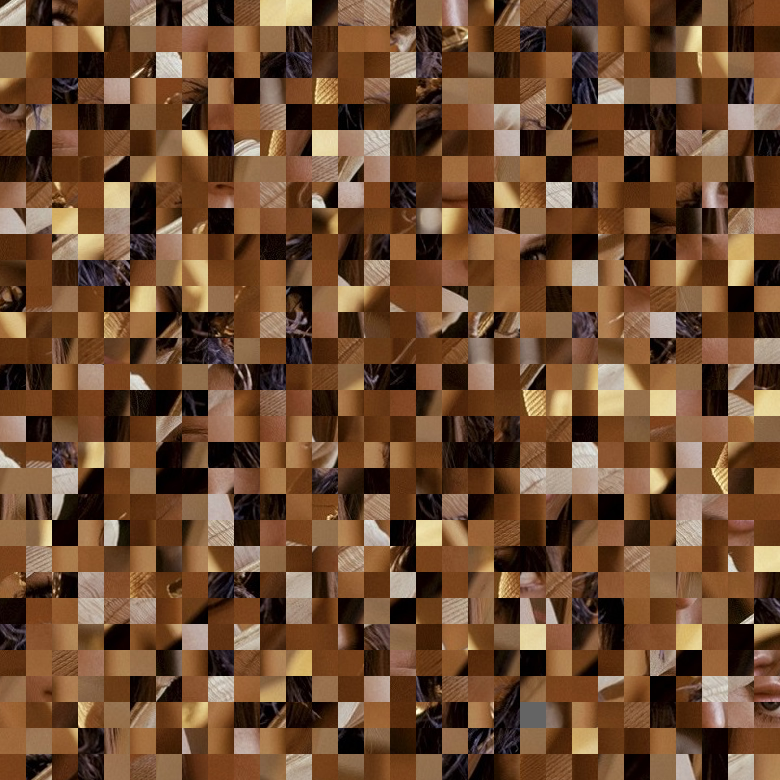
\includegraphics[width=0.35\linewidth]{img/dsf-1.png}
    }
    \quad\quad
    \subfloat[Puzzle nach Spanning-Tree Algorithmus\label{fig-dsf-stages-2}]{
      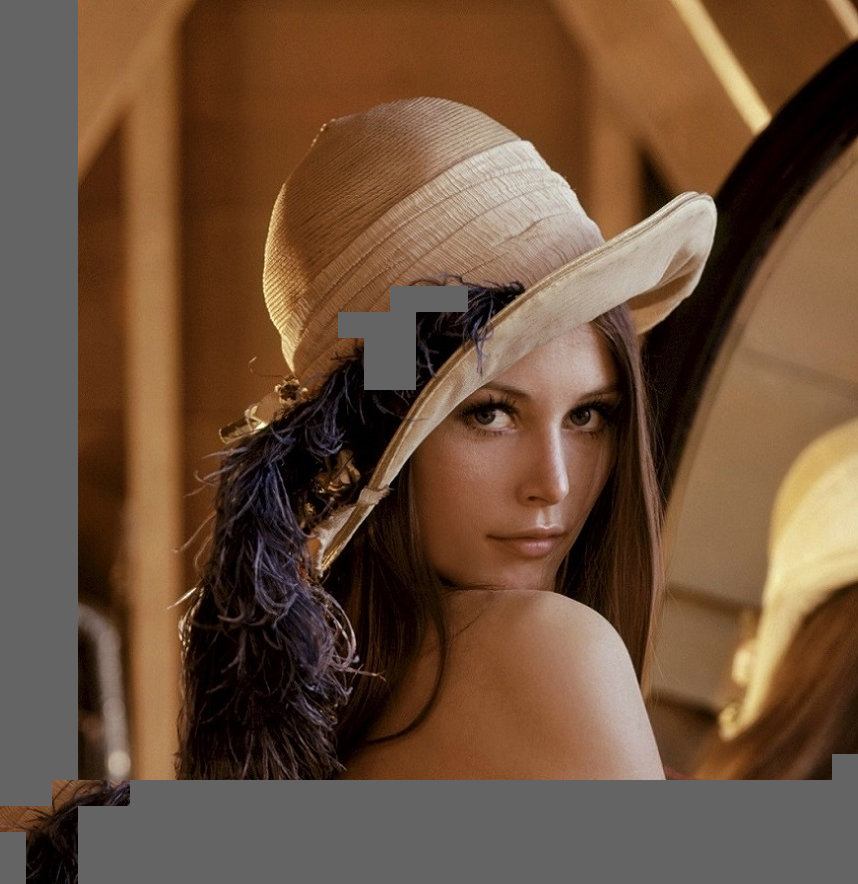
\includegraphics[width=0.35\linewidth]{img/dsf-2.png}
    }
    \\
    \subfloat[Puzzle nach Trimming\label{fig-dsf-stages-3}]{
        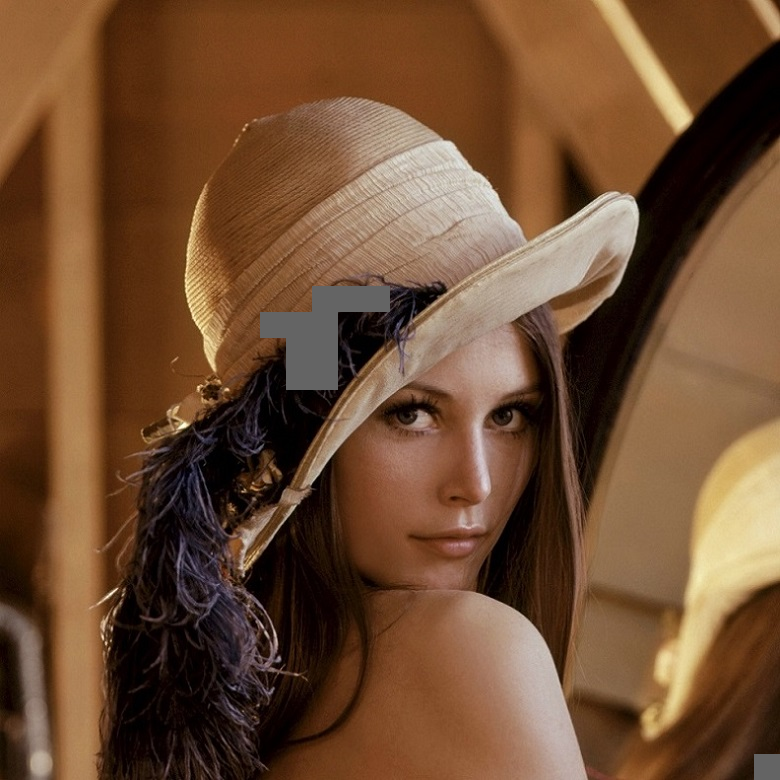
\includegraphics[width=0.35\linewidth]{img/dsf-3.png}
    }
    \quad\quad
    \subfloat[Puzzle nach Filling\label{fig-dsf-stages-4}]{
        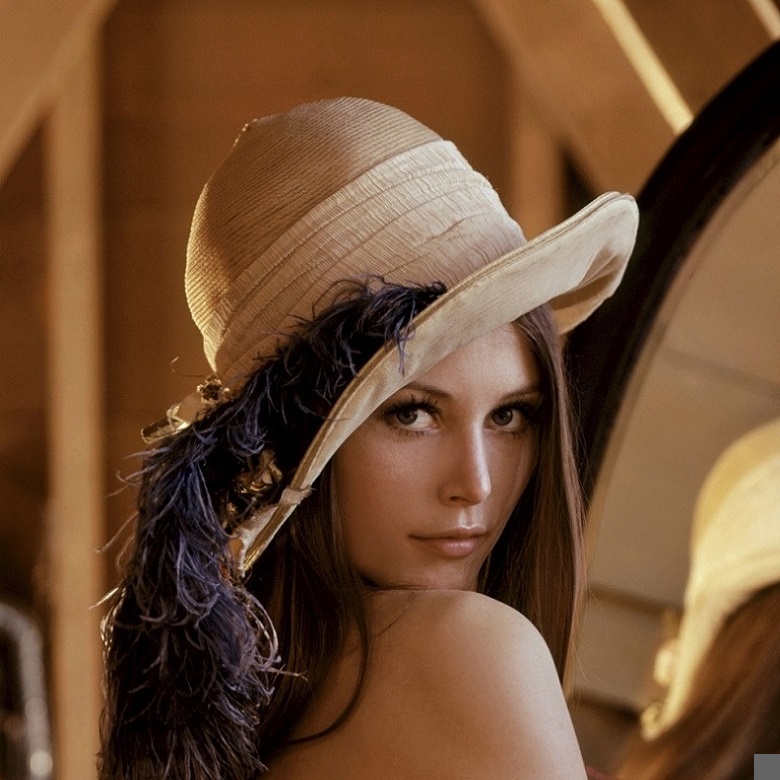
\includegraphics[width=0.35\linewidth]{img/dsf-4.png}
    }
    \caption{Die 4 Stages eines Puzzles im Gesamtalgorithmus}
    \label{fig-dsf-stages}
\end{figure}
\section{Trimming}
Sobald nur noch eine Zusammenhangskomponente im Forest vorhanden ist, lässt sich die Wurzel dieses Spannbaums im Array auffinden. Diese Wurzel kennt alle Elemente inklusive den relativen Koordinate zu sich selbst. Mit den minimalen und maximalen x- und y-Koordinaten aller Elemente lässt sich die Anzahl der nötigen Zeilen und Spalten bestimmen, um alle Elemente in einem Rechteck darzustellen. Der Punkt mit der minimalen x-Koordinate aller Elemente und der minimalen y-Koordinate aller Elemente (die obere-linke Ecke des Rechtecks) wird Urpsrung des neuen Koordinatensystems. Durch eine simple Vektordifferenz zwischen den Wurzelkoordinaten eines Elementes und den Koordinaten dieses Ursprungs (auch in Wurzelkoordinaten) ergibt sich die Koordinate eines Elementes in dem neuen Frame. Das Ergebnis dieser Rekonstruktion ist in Abbildung \ref{fig-dsf-stages-2} dargestellt.

Aus diesem Zwischenergebnis soll dann ein Rechteck extrahiert werden, welches die Dimensionen des Puzzles besitzt. Dazu wird dem Algorithmus diese Information mitgeteilt (Anzahl der Zeilen und Spalten vom Puzzle). Dieser legt dann eine Art Sliding-Window über das zuvor rekonstruierte Puzzle und summiert die Anzahl der belegten Puzzlefelder auf. Die Position, die ein Puzzle ergeben würde, was am dichtesten gefüllt ist (also am meisten Stücke platziert sind), wird als beste Position definiert.

Im nächsten Schritt wird das Puzzle aus \ref{fig-dsf-stages-2} so getrimmt, dass der Teil des Puzzles, welcher sich innerhalb dieses Sliding-Windows (welches an der zuvor bestimmten Position angebracht wird) befindet, in ein neues Zwischenergebnis übernommen wird. Das dabei entstehende Bild besitzt nun die gewünschten Dimensionsgrößen, enthält aber noch nicht belegte Plätze (vgl. Abbildung \ref{fig-dsf-stages-3}). Alle Stücke die nicht übernommen wurden, werden in einer Menge zwischengespeichert. Es gilt nun im nächsten Schritt, alle Stücke dieser Menge bestmöglich auf die freihen Plätze des Puzzles zu verteilen.
\section{Filling}
Bevor das Puzzle gefüllt wird, sollen zunächst die möglichen Plätze für Stücke analyisert werden. Die freien Plätze werden dabei in $5$ Buckets eingeteilt: Buckets $0\dots4$. Die Nummer des Bucket steht für die Anzahl der benachbarten belegten Felder. Die Idee dabei ist, zunächst die Buckets in absteigender Reihenfolge abzuarbeiten, da die Felder mit mehr Nachbarn auch mehr Informationen darüber liefern können, wie gut ein Stück in das Feld passt. Außerdem gilt zu beachten, dass im Laufe dieses Verfahren Puzzlestücke aus den niedrigen Buckets durch das Füllen der Plätze wiederum Nachbarn bekommen und somit solange \textit{promoted} werden, bis diese Stücke selber platziert werden.

Dieses Verfahren funktioniert wie von \cite{gallagher,crisjim} gezeigt, gut für Puzzle, die keine fehlenden Puzzlestücke haben. Damit ist dies der erste (und auch einzige Schritt) im ganzen Algorithmus, der hier leicht abgeändert werden muss. Schließlich fehlt bei Schiebepuzzles immer exakt ein Puzzlestück. Der Algorithmus wird dementsprechend angepasst. Es sei aber gesagt, dass dieses Verfahren nicht gut erweiterbar ist auf mehrere fehlende Puzzlestücke. Diese Problemstellung ist ein viel schwierigeres Problem, welches auch schon entsprechend Aufmerksamkeit in der Literatur bekommen hat. \cite{paikin}

Die ursprüngliche Idee ist es, alle Kombinationen aus noch nicht platzierten Stücken und freien Plätzen eines Buckets durchzuprobieren. Dabei wird in jedem Durchgang der höchste Bucket ausgewählt, der mindestens ein Element enthält. Durch die gleichen Distanzen welche auch schon für den Hauptalgorithmus genommen wurden, lässt sich vergleichen, wie gut ein Puzzlestück in ein freies Feld passt. Es wird wieder Greedy vorgegangen, womit das beste Paar aus Puzzlestück und Platz kombiniert werden. Das Stück wird platziert und aus der Menge entfernt. Auch der (nun nicht mehr) freie Platz wird aus seinem entsprechenden Bucket platziert. Außerdem werden dabei ggf. die Nachbarn des Platzes aktualisiert. Befinden sich dort freie Plätze, so können diese alle einen Bucket höher platziert werden (da ein freier Nachbarplatz nun gefüllt wurde). Dieser Vorgang wird so lange wiederholt, wie sich noch nicht platzierte Stücke in der Menge befinden.

An dieser Stelle ist klar, dass dies bei einem Schiebepuzzle ziemlich schief gehen kann. Ist das freie Feld des Schiebepuzzles beispielsweise von keinen freien Feldern umgeben, hat dieses (selbst wenn es schlechte Kompatibilitäten mit den Puzzlestücken aufweist) eine so hohe Priorität bearbeitet zu werden, dass es mit großer Wahrscheinlichkeit trotzdem fälschlicherweise gefüllt wird. Abbildung \ref{fig-dsf2} zeigt ein Beispiel solch eines Fehlers.
\begin{figure}[H]
    \centering
    \subfloat[Gewünschte Lösung\label{fig-dsf2-1}]{
      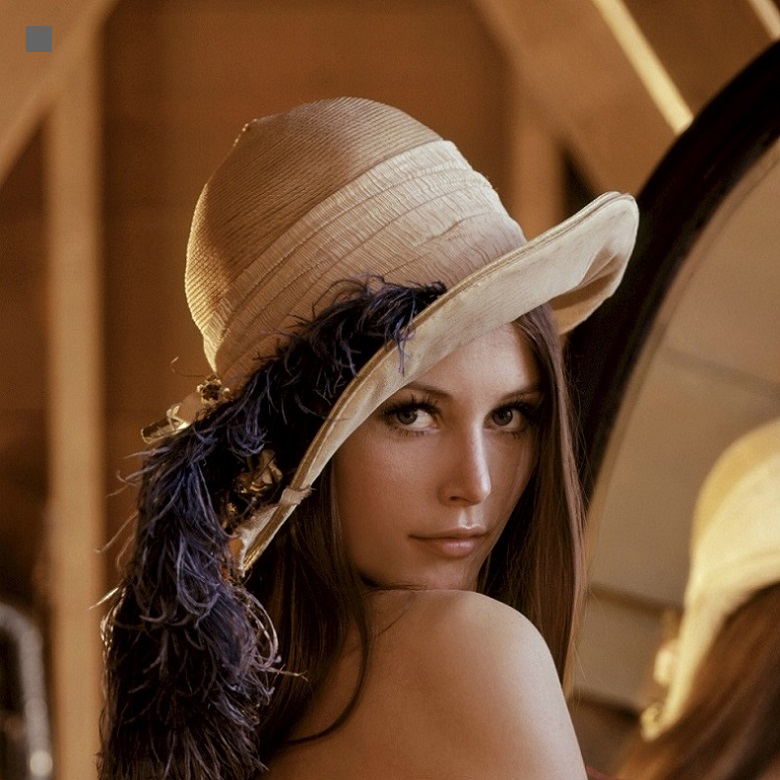
\includegraphics[width=0.50\linewidth]{img/dsf2-1.png}
    }
    \subfloat[Lösung mit falschem Filling\label{fig-dsf2-1}]{
      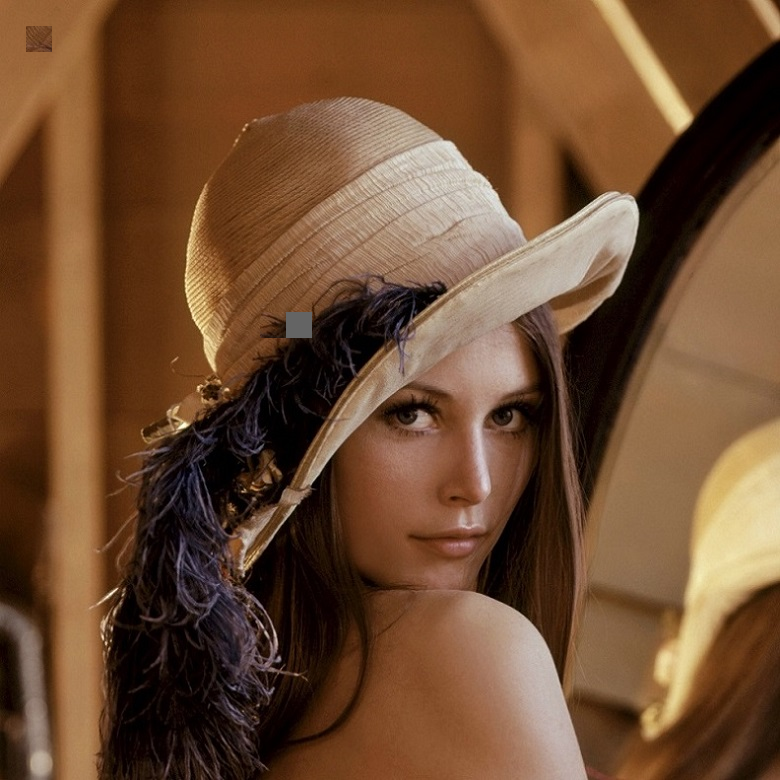
\includegraphics[width=0.50\linewidth]{img/dsf2-2.png}
    }
    \caption{Fehler beim Filling Algorithmus}
    \label{fig-dsf2}
\end{figure}
Um dieses Problem zu lösen, wird das Verfahren nur leicht angepasst. Anstatt den höchsten Bucket mit mindestens einem Element zu nehmen (was dazu führt, dass dieser Platz auf jeden Fall belegt wird, was wiederum zu den Fehler in Abb. \ref{fig-dsf2} führt), wird der höchste Bucket mit mindestens zwei Elementen genommen und sofern ein höherer Bucket mit exakt einem Element existiert, dann konkurriert dieses Element mit allen Elementen des niedrigeren Buckets. Existiert der freie Platz des Schiebepuzzles etwa in Bucket 4, so würden zunächst alle anderen freien Plätze mit vier Nachbarn vergeben werden sofern die Metrik stimmt (da es kein passendes Stück für diesen Platz gibt). Danach ist dieses Element alleine im Bucket, wird aber nicht automatisch ausgewählt, sondern wird jetzt zusammen mit den Elementen aus Bucket 3 gegen die noch nicht platzierten Stücke verglichen. Somit ist sichergestellt, dass das Element was am Ende der Prozedur über bleibt, nicht irgendein Element ist, sondern das Element, was im Vergleich zu allen anderen Elementen immer die schlechteste Kompatibilität mit den Puzzlestücken hatte.
\section{Kanten-Vorverarbeitung}
An dieser Stelle sind noch zwei Dinge zu erledigen, die einerseits die Qualität des Algorithmus verbessern und andererseits die Laufzeit durchschnittlich verringern.

Da der Algorithmus keine Form von Backtracking hat (außer in Form von Trimming \& Filling), kann selbst eine einzige falsche Zuordnung von Puzzleteilen, welche sehr früh im Algorithmus auftritt, später zu sehr falschen Ergebnissen führen. Intuitiv lässt sich das damit begründen, dass der Fehler nie behoben werden kann (zwei verbundene Stücke bleiben immer verbunden) und der Algorithmus somit um den Fehler herumarbeiten muss, wodurch weitere falsche Entscheidungen getroffen werden (die in diesem Zeitpunkt als das geringste Übel aussehen und der Algorithmus schließlich greedy vorgeht). Damit pflanzen sich diese Fehler immer weiter fort. Dies ist besonders bei Bildern der Fall, wo viele Stücke ähnlich gute Kompatibilitäten zueinander besitzen. Beispielsweise Puzzlestücke mit Teilen vom Himmel oder wo nur Wasser abgebildet ist. Um diesem Effekt entgegenzuwirken werden die Distanzen der Puzzlestücke nach der initialen Berechnung angepasst. Dazu wird zu jedem Paar von Puzzlestück und Position des Puzzlestücks die Kante mit der zweitniedrigsten Distanz aller dieser Kanten ermittelt (beispielsweise die Kante mit der zweitbesten Distanz von allen Kanten die bei denen ein Teil $x_i$ links vom anderen Puzzlestück liegt).\cite{gallagher,crisjim} Damit werden die Kantengewichte so normalisiert, dass nur die besten Kanten eine Distanz $<1$ aufweisen und alle anderen Distanzen nun $\geq1$ sind. Damit würde der Algorithmus in einem Bild mit einem klaren Himmel also nicht probieren zunächst diesen Himmel komplett anzuordnen (obwohl die Kanten dort sehr niedrige absolute Distanzen aufweisen), was mit hoher Wahrscheinlichkeit nicht fehlerlos passieren würde.

Da die Datenstruktur fast den kompletten Algorithmus übernimmt, muss der eigentliche Algorithmus (Kruskal) nur über die Kanten iterieren und die entsprechende \texttt{Union} Operation der Datenstruktur aufrufen, sofern noch kein Spannbaum entstanden ist. Da die Kanten in aufsteigender Reihenfolge (bezüglich der Distanz) abgearbeitet werden sollen, wird dafür oft zunächst die Kantentabelle sortiert (was $\Theta(|E|\log|E|)$ ist). Da der Graph des Puzzles jedoch unglaublich dicht ist (jedes Paar zweier Vertices wird durch $4$ Kanten verbunden), werden nur ein Bruchteil dieser Kanten benötigt, um den Graphen zu spannen. Daher bietet es sich an eine Priority-Queue zu verwenden, womit zunächst nur ein $\Theta(|E|)$ Aufwand nötig ist, um die Heapbedingung der Kantentabelle herzustellen und dann das Entfernen einer Kante dann $\mathcal{O}(\log|E|)$ ist. Selbst in dem Fall, dass doch fast alle Kanten betrachtet werden müssen ist dieser Ansatz von der Komplexität her trotzdem nicht schlechter als der Ansatz mit vorherigem Sortieren, da es sich dann lediglich ein Heapsort ergibt, welcher optimales Laufzeitverhalten besitzt.
\section{Ergebnis}
Wie bereits in Abbildung \ref{fig-dsf-stages} gezeigt wurde, ist der Algorithmus in der Lage Puzzles von bis zu 1000 Puzzlestücken (die Abbildung zeigt in $30\times30$ Beispiel) perfekt zu lösen. Diese Genauigkeit ist zu einem großen Teil der MGC-Metrik \ref{section-mgc} zu verdanken. Puzzles mit bis zu 1000 Stücken werden aufgrund einer effizienten Implementation der Datenstruktur in wenigen Sekunden assembliert. Mögliche Verbesserungen und Erweiterungen bezüglich der Genauigkeit, Laufzeit und auch Speicherverbrauch (zur Speicherung der berechneten Distanzen zwischen Puzzlestücken) sind für das Lösen von sehr großen Puzzles (mehrere tausend Stücke) möglich, jedoch hier nicht nötig. Mit der Hauptmotivation diese Assemblierung als Zwischenschritt für das Lösen von Bild-Schiebepuzzles zu verwenden, sollte bewusst sein, dass die Anzahl der Puzzlestücke von Schiebepuzzles in der Regel nicht viel mehr als etwa $20$ sein dürfen, sofern dieses Puzzle optimal von einem Suchalgorithmus gelöst werden soll.
\chapter{Lösbarkeit eines Schiebepuzzles}\label{ch-perm}
In diesem Kapitel wird kurz erklärt, wie geprüft werden kann, ob ein Schiebepuzzle mit einem bestimmten Anfangszustand und einem bestimmten Endzustand lösbar ist. Mit den Ergebnissen der vorherigen Kapitel lässt sich ein $m\times n$ Puzzle aus einer Menge von $N-1=mn-1$ Puzzlestücken zusammensetzen. Diese Zusammensetzung wird als Endzustand anerkannt. Der Startzustand sei beliebig, weshalb deshalb von Interesse ist, ob und wann es überhaupt möglich ist durch eine Reihe von legalen Zügen einen Startzustand in den Endzustand zu bringen. Im Zusammenhang damit ist dann auch interessant, wie sich aus einem Bild (und damit mit einem festen Endzustand) Startzustände generieren lassen, welche immer lösbar sind (dies ist nützlich um Algorithmen zur Lösung des Puzzles zu testen).

Dazu wird angenommen, dass die $N-1$ Puzzlestücke von $1$ bis $N-1$ nummeriert sind (das leere Feld im Puzzle wird als $0$ definiert). Sowohl der Anfangs- als auch der Endzustand ist dann lediglich eine Permutation dieser Zahlen. Es werden dann für beide Zustände die Permutation betrachtet, die beim abtragen der Zahlen in Leserichtung (also von oben nach unten und innerhalb einer Zeile von links nach rechts) entsteht. Das freie Feld wird dabei ignoriert. Damit entstehen für beide Zustände eine Permutation der Form $\alpha,\beta:\{1,\dots,N-1\}\longrightarrow\{1,\dots,N-1\}$.

Zwischen diesen beiden Permutationen wird die Kendall-Tau-Distanz betrachtet, welche die Summe aller Paare der beiden Permutationen zählt, welche nicht in der gleichen Reihenfolge in den Permutationen vorkommt. Es wird also jedes Paar gezählt, dessen Reihenfolge in den beiden Permutationen verschieden ist. Die Kendall-Tau-Distanz zwischen den beiden Permutationen $(2,1,4,3)$ und $(4,1,3,2)$ ist beispielsweise $4$, da die folgenden Paare an Zahlen in verschiedener Reihenfolge in den beiden Permutationen auftreten: $(1,2),(1,4),(2,3),(2,4)$. Formal lässt sich die Kendall-Tau-Distanz folgendermaßen für die beiden Permutationen $\alpha,\beta$ berechnen:\cite{sedge}
\begin{align}\label{eq-kendall}
    K(\alpha,\beta)=\sum_{0<i<j<N}\left[\beta^{-1}\left(\alpha\left(i\right)\right)>\beta^{-1}\left(\alpha\left(j\right)\right)\right]
\end{align}
Wobei $[\cdot]$ für das Iverson-Bracket steht, welches $1$ ergibt, wenn die Bedingung in den eckigen Klammern erfüllt ist und $0$ wenn nicht.

Substituiert man nun $\pi=\beta^{-1}\circ\alpha$, erhält man die Definition der Anzahl der Inversionen einer Permutation:\cite{inv}
\begin{align}\label{eq-inv}
    inv(\pi)=\sum_{0<i<j<N}[\pi(i)>\pi(j)]
\end{align}
Der Zusammenhang dieser beiden Operationen ist, dass die Anzahl der Inversionen einer Permutation die Kendall-Tau-Distanz dieser Permutation mit der Identitätspermutation $id(x)=x$ darstellt.

Die Substitution bewirkt quasi, dass man nun zwei andere Zustände der Schiebepuzzle hat (bezüglich der Zahlenwerte her, das leere Feld bleibt unverändert), indem man den Endzustand als Identitätspermutation definiert hat. Der Startzustand wird durch die Permutation $\pi$ repräsentiert. Ein $\pi(k)$ ist dann anschaulich der Index aus $\beta$ an dem der Wert $\alpha(k)$ steht. Hat unser alte Anfangszustand beispielsweise die Zahl $5$ im ersten Feld (erste Zeile, erste Spalte) und befindet sich die $5$ im Endzustand im dritten Feld (erste Zeile, dritte Spalte), so steht der Wert $3$ im ersten Feld des neu definierten Anfangszustands. Diese Umbenennung dient lediglich der einfacheren Handhabung einer Permutation (und einer impliziten Identitätspermutation).

Um das Schiebepuzzle zu lösen, ist es notwendig die Permutation $\pi$ in die Identitätspermutation zu transformieren. Dies ist noch nicht hinreichend, weil dann noch sichergestellt werden muss, dass nicht nur die Reihenfolge der Zahlenwerte stimmt, sondern auch das leere Feld sich an der richtigen Stelle befindet.

Da die Anzahl der Inversionen einer Permutation nur dann gleich $0$ sind, wenn es sich um die Identitätspermutation handelt, lässt sich auch sagen, dass das Ziel ist $inv(\pi)$ auf $0$ zu bringen.

Beim Schiebepuzzle sind zwei Arten von Zügen zugelassen: Züge innerhalb einer Zeile und Züge innerhalb einer Spalte. An dieser Stelle lässt sich der Vorteil der Repräsentation als Permutation ohne leeres Feld erkennen, denn ein Zug innerhalb einer Zeile des Puzzles ändert nichts an der Permutation und somit auch nichts an der Anzahl der Inversionen der Permutation.

Für Spaltenzüge wird ein Puzzlestück betrachtet mit Koordinaten $(i,j)$, wobei $i$ der nullbasierte Zeilenindex ist und $j$ der nullbasierte Spaltenindex. Der nullbasierte Index $k$ in Leserichtung (und diesmal mit dem leeren Element) berechnet sich zu $k=n\:i+j$. Soll dieses Stück innerhalb seiner Spalte bewegt werden, so muss sich das leere Element an der Stelle $(i\pm1,j)$ befinden oder auch $l=n\:(i\pm1)+j$. Die Anzahl der Elemente zwischen dem Puzzlestück und dem leeren Feld ist $|k-l|-1=|n\:i+j-[n\:(i\pm1)+j]|-1=|\mp n|-1=n-1$. In der Permutation bedeutet dies, dass das Puzzlestück um $n-1$ Stellen nach links oder rechts rutscht. Damit ändert sich die relative Position von diesem Puzzlestück mit jedem der $n-1$ Elemente: Hat eines der Elemente vorher eine Inversion mit dem Stück gebildet, so ist dies jetzt nicht mehr der Fall und umgekehrt auch. Die Anzahl der Inversionen ändert sich also. Es gilt
\begin{align}\label{eq-parity}
    inv(\pi^\prime)=inv(\pi)\underbrace{\pm1\pm1\pm\dots\pm1\pm1}_{n-1\text{ mal}}
\end{align}
An dieser Stelle wird unterschieden zwischen Schiebepuzzles mit einer geraden Anzahl von Spalten geraden $n$ und Schiebepuzzles mit einer ungeranden Anzahl an Spalten.

Für ungerade $n$ ist $n-1$ gerade. Da eine Summe mit einer geraden Anzahl an ungeraden Summanden stets gerade ist, ist der Ausdruck über der geschweiften Klammer in \ref{eq-parity} somit auch gerade. Dann ist die Parität von $inv(\pi^\prime)$ aber gleich der Parität von $inv(\pi)$. Anders gesagt gilt$$inv(\pi^\prime)\equiv inv(\pi)\pmod2$$
Damit ändert sich die Anzahl der Inversionen für ungerade $n$ bei einem Zeilenzug garnicht womit die Parität der Anzahl der Inversionen trivialerweise gleich bleibt. Und da diese auch bei einem Spaltenzug gleich bleibt, lässt sich sagen, dass die Parität der Anzahl der Inversionen einer Permutation unter allen legalen Zügen des Schiebepuzzles invariant ist. Um die Anzahl der Inversionen also auf $0$ (eine gerade Zahl) bringen zu können (und das Puzzle damit zu lösen), muss die Permutation des Anfangszustand eine gerade Anzahl an Inversionen aufweisen.

Im anderen Fall ($n$ ist ungerade), lässt sich sagen, dass die Summe über der geschweiften Klammer in \ref{eq-parity} stets ungerade ist, wodurch sich die Parität mit jedem Spaltenzug ändert. Deshalb werden für ungerade $n$ auch noch die Zeilenindizes $r,s$ der leeren Felder in beiden Zuständen betrachtet. Um das Puzzle zu lösen ist es auch notwendig das leere Feld an der richtigen Stelle zu haben (und damit besonders in der richtigen Zeile). Betrachtet man den Zeilenabstand der beiden leeren Felder, also $|r-s|$, so ist klar, dass auch dieser notwendigerweise $0$ sein muss. Dieser Zeilenabstand ändert sich aber bei jedem Spaltenzug um $\pm1$. Damit ändert sich die Parität von $|r-s|$ bei jedem Spaltenzug. Zusammengefasst lässt sich schließen, dass die Puzzles mit ungeraden $n$ die Parität der Anzahl der Inversionen gleich der Parität des Zeilenabstand beider leeren Felder sein muss. Da beide Attribute auf $0$ gebracht werden müssen beim Lösen und somit am Ende auf eine gerade Parität kommen müssen, beide aber in jedem Spaltenzug ihre Parität ändern, würde eine ungleiche Parität der beiden dazu führen, dass in jedem Schritt genau einer von beiden dafür sorgt, dass das Puzzle nicht gelöst sein kann.

Die obigen Bedingungen müssen damit notwendigerweise von lösbaren Schiebepuzzles erfüllt sein. Die andere Richtung (dass diese Bedingungen tatsächlich auch hinreichend sind) wurde von Johnson \& Story \cite{fift} gezeigt. Dementsprechend gilt für alle Schiebepuzzle, dass diese dann und nur dann lösbar sind, wenn diese die obigen Bedingungen erfüllen. Tatsächlich wurde in diesem Paper auch gezeigt, dass die Menge aller Puzzlezustände sich in zwei gleich große Äquivalenzklassen partitionieren lässt. Die Zustände dieser Äquivalenzklassen lassen sich stets unter Verwendung legaler Züge nur in andere Zustände der selben Äquivalenzklasse transformieren. Damit ist immer genau die Hälfte aller Permutationen eines Schiebepuzzles lösbar.

Um die Lösbarkeit eines Schiebepuzzles zu bestimmen muss also lediglich die Parität der Anzahl der Inversionen der Permutation des Schiebepuzzles (und je nach Spaltenanzahl auch noch die Parität des Zeilenabstandes der beiden leeren Felder) überprüft werden. Da diese Überprüfungen alle konstant sind, hängt die Laufzeit- und Speicherkomplexität lediglich von der Bestimmung der zusammengesetzten Permutation $\pi$ ab (dies ist ein linearer Zeit mit linearem Speicher möglich) und der Berechnung der Parität.

Eine triviale Möglichkeit die Parität zu bestimmen basiert auf der Berechnung der Inversionen nach Gleichung \ref{eq-inv}. Da die Summe jedoch über $\binom{N-1}{2}$ geht, ist die Laufzeitkomplexität hier mit $\Theta(N^2)$ quadratisch. Dafür wird aber an dieser Stelle nicht noch weiterer zusätzlicher Speicher benötigt.

Eine Möglichkeit die Anzahl der Inversionen zu bestimmen ergibt sich durch eine Erweiterung des Mergesort-Algortihmus.\cite{sedge} Die Permutation wird in zwei gleich große Hälften zerlegt. Die gesamte Anzahl an Inversionen lässt sich dann in drei Summanden zerlegen: Alle Inversionen die in der linke Hälfte auftreten, alle Inversionen die in der rechten Hälfte auftreten und alle Inversionen, die übergreifend der Hälften auftreten. Die ersten beiden Summanden ergeben sich durch die Rekursion (der Basisfall der Rekursion sind Permutation mit weniger als zwei Elementen, welche trivialerweise keine Inversionen haben können). Die Inversionen, welche zwischen den beiden (nun auch sortierten) Hälften auftreten, lassen sich in dem Merge-Schritt des Algorithmus mitzählen. Da jedes Element aus der linken Hälfte in der Permutation vor jedem Element aus der rechten Hälfte kam, so entstehen genau dann Inversionen, wenn das aktuell betrachtete Element aus der rechten Hälfte kleiner ist als das aktuell betrachtete Element aus der linken Hälfte. Dieses Element der rechten Hälfte bildet dann mit allen verbleibenden Elementen der linken Hälfte eine Inversion, da es in der Permutation zwar rechts von diesen Elementen stand, jedoch kleiner als alle dieser Elemente ist. Es folgt ein Beispiel mit der Permutation $\pi=(3,4,7,9,2,5,6,8)$. Beide Hälften $\lambda=(3,4,7,9),\mu=(2,5,6,8)$ sind bereits sortiert, womit innerhalb der beiden Hälften keine Inversionen auftreten. Es gilt nun diese zusammenzufügen, um die Inversionen zwischen den beiden Hälften zu zählen.
\begin{align*}
    \lambda&=(3,4,7,9),&\mu&=(\underline{2},5,6,8),&\pi^\prime&=(),&inv(\pi)&=0\\
    \shortintertext{$2$ ist das Minimum und bildet mit allen restlichen Elementen aus $\lambda$ eine Inversion. Damit ergeben sich $4$ Inversionen beim Merge.}
    \lambda&=(\underline{3},4,7,9),&\mu&=(\cancel{2},5,6,8),&\pi^\prime&=(2),&inv(\pi)&=4\\
    \shortintertext{Das nächste Minimum kommt aus der linken Hälfte und bildet somit keine neuen Inversionen.}
    \lambda&=(\cancel{3},\underline{4},7,9),&\mu&=(\cancel{2},5,6,8),&\pi^\prime&=(2,3),&inv(\pi)&=4\\
    \lambda&=(\cancel{3},\cancel{4},7,9),&\mu&=(\cancel{2},\underline{5},6,8),&\pi^\prime&=(2,3,4),&inv(\pi)&=4\\
    \shortintertext{$5$ bildet mit den restlichen beiden Elementen aus $\lambda$ (Elemente $7,9$) Inversionen.}
    \lambda&=(\cancel{3},\cancel{4},7,9),&\mu&=(\cancel{2},\cancel{5},\underline{6},8),&\pi^\prime&=(2,3,4,5),&inv(\pi)&=6\\
    \lambda&=(\cancel{3},\cancel{4},\underline{7},9),&\mu&=(\cancel{2},\cancel{5},\cancel{6},8),&\pi^\prime&=(2,3,4,5,6),&inv(\pi)&=8\\
    \lambda&=(\cancel{3},\cancel{4},\cancel{7},9),&\mu&=(\cancel{2},\cancel{5},\cancel{6},\underline{8}),&\pi^\prime&=(2,3,4,5,6,7),&inv(\pi)&=8\\
    \lambda&=(\cancel{3},\cancel{4},\cancel{7},\underline{9}),&\mu&=(\cancel{2},\cancel{5},\cancel{6},\cancel{8}),&\pi^\prime&=(2,3,4,5,6,7,8),&inv(\pi)&=9\\
    \lambda&=(\cancel{3},\cancel{4},\cancel{7},\cancel{9}),&\mu&=(\cancel{2},\cancel{5},\cancel{6},\cancel{8}),&\pi^\prime&=(2,3,4,5,6,7,8,9),&inv(\pi)&=9
\end{align*}
Es ergibt sich für $\pi$ eine Inversionszahl von $9$.

Der Algorithmus besitzt somit die gleichen Eigenschaften wie ein normaler Mergesort, womit sich eine Laufzeitkomplexität von $\Theta(N\log N)$ ergibt. Es ist zusätzlich noch linearer Speicheraufwand nötig (für das temporäre Array, welches zum Mergen benötigt wird). Da die Berechnung der zusammengesetzten Permutation $\pi$ jedoch bereits linearen Speicher braucht, ändert dies nichts an der Speicherkomplexität der kompletten Prozedur.

Um die komplette Prozedur sowohl in Zeit, als auch in Speicher linear zu halten, muss ein anderer Ansatz her. Die entscheidende Beobachtung dafür ist, dass die exakte Anzahl der Inversionen garnicht nötig ist und lediglich die Parität dieser Anzahl eine Rolle spielt. Diese Parität der Inversionen wird tatsächlich als Parität der Permutation definiert und es gibt viele equivalente Definitionen der Parität einer Permutation. Eine dieser Definitionen definiert die Parität einer Permutation als die Parität der Anzahl der Transpositionen\footnote{Eine Transposition $\tau_{a,b}$ ist eine Permutation, welche zwei Elemente tauscht (also $a$ auf $b$ abbildet und $b$ auf $a$ abbildet) und alle anderen Elemente gleich lässt (also alle anderen Elemente $c$ wiederum auf $c$ abbildet).}, die nötig sind, um die Identitätspermutation in diese Permutation zu transformieren. Es sei zu beachten, dass die Anzahl der Transpositionen dabei (im Gegensatz zu der Annzahl der Inversionen) für eine Permutation nicht eindeutig ist. Die Parität dieser Anzahl ist jedoch immer gleich. Eine Permutation die beispielsweise $5$ Transpositionen benötigt, lässt sich auch in $7$ Transpositionen erstellen, indem am Ende der ersten $5$ noch eine willkürliche Transposition durchgeführt wird und dann sofort die inverse dieser Transposition angewendet wird.

Um die Äquivalenz der beiden Definitionen zu zeigen wird ein induktiver Ansatz gewählt. Offensichtlich lässt sich die Identitätspermutation durch das anwenden von $0$ Transpositionen in die Identitätspermutation transformieren. Außerdem hat die Identitätspermutation auch $0$ Inversionen, beide Definitionen liefern also die gleiche Parität. Sind beide Paritäten für eine Permutation $\pi$ nun gleich und wird eine beliebige Transposition $\tau_{\pi(i),\pi(j)}$ mit $i<j$ auf $\pi$ angewandt, so erhöht sich die Anzahl der Transpositionen um $1$ und $\tau_{\pi(i),\pi(j)}\circ\pi$ besitzt die inverse Parität von $\pi$. Nun gilt es zu betrachtet, was mit $inv(\pi)$ bei der Anwendung der Transposition passiert. Alle Inversionen der Permutation mit Elementen links von $i$ oder rechts von $j$ bleiben bei der Transposition erhalten. Nun befinden sich zwischen $i$ und $j$ genau $h=j-i-1$ Elemente. Jedes dieser Elemente könnte sowohl mit dem Element an der Stelle $i$, als auch mit dem Element an der Stelle $j$ eine Inversion gebildet haben. Sei nun $p$ die Anzahl dieser Elemente, welche eine Inversion mit dem Element an der Stelle $i$ gebildet haben und $q$ die Anzahl der Elemente, die eine Inversion mit $j$ formen. Beim Durchführen der Transposition gehen somit $p+q$ Inversionen verloren, es entstehen aber dafür $(h-p)+(h-q)$ neue Inversionen. Nun ist noch zu beachten, dass die Elemente an den Stellen $i$ und $j$ selber ihre relative Position ändern und somit die Anzahl der neuen Inversionen entweder inkrementieren oder dekrementieren. Die neue Anzahl der Inversionen ist also $inv(\tau_{\pi(i),\pi(j)}\circ\pi)=inv(\pi)-(p+q)+(h-p)+(h-q)\pm1=inv(\pi)+2h-2p-2q\pm1=inv(\pi)+2(h-p-q)\pm1$. Es wird also eine ungerade Zahl auf die (alte) Anzahl der Inversionen addiert. Damit ändert sich die Parität der Anzahl der Inversionen bei jeder Anwendung einer Transposition. Da beide Definition für die Identitätspermutation die gleiche Parität liefern, die Anwendung jeder Transposition auf eine Permutation beide Paritäten invertiert und jede Permutation sich als die Komposition endlich vieler Transpositionen darstellen lässt, sind beide Definitionen der Parität einer Permutation für alle Permutationen gleich.

Es reicht also, einen Algorithmus zu finden, der eine (beliebige) Zerlegung einer Permutation in Transpositionen findet. Die Anzahl dieser Transpositionen könnte sich zählen lassen, womit die Parität bekannt wäre. Dazu wird noch eine finale Eigenschaft von Permutationen betrachtet.

Permutationen lassen sich (da diese bijektive Funktionen sind) in disjunkte Zyklen zerlegen. Die Permutation $\pi=(3,6,1,2,5,4)$ bildet etwa $1$ auf $3$ ab, $3$ wird aber wiederum auf $1$ abgebildet, womit der Zyklus $(1,3)$ entsteht (dies entspricht einer Transposition). Auch gilt $2\mapsto6,6\mapsto4,4\mapsto2$ womit der nächste Zyklus $(2,6,4)$ ensteht. Als letztes wird $5$ auf $5$ abgebildet, was auch ein Zyklus darstellt $(5)$ (ein sogenannter \textit{fixed-point}). Die Permutation kann dann als das Produkt solcher Zyklen ausgedruckt werden (Zyklenschreibweise). Eine Möglichkeit dies auszudrücken wäre nach oben dann $\pi=(1,3)(2,6,4)(5)$.

Ein Zyklus $\sigma=(a_1,a_2,\dots,a_k,\dots,a_{n-1},a_n)$ der Länge $n$ lässt sich aber als die Komposition von Transpositionen darstellen. Von besonderem Interesse ist die Anzahl der Transpositionen die dafür nötig sind. Diese ist zwar nicht klar definiert, die Parität der Anzahl aber schon, womit es hinreichend ist eine solche Komposition zu finden. Zwei solcher Kompositionen wären beispielsweise $\sigma=\tau_{a_1,a_n}\circ\tau_{a_1,a_{n-1}}\dots\circ\tau_{a_1,a_k}\dots\circ\tau_{a_1,a_3}\circ\tau_{a_1,a_2}$ oder auch $\sigma=\tau_{a_1,a_2}\circ\tau_{a_2,a_3}\circ\dots\tau_{a_k,a_{k+1}}\dots\circ\tau_{a_{n-2},a_{n-1}}\circ\tau_{a_{n-1},a_n}$. Beide Zerlegungen haben die Länge $n-1$.

Eine Permutation lässt sich also in disjunkte Zyklen zerlegen, welche sich alle wiederum in Transpositionen zerlegen lassen können. Die Parität der Anzahl aller Transpositionen ist dann die gesuchte Parität der Permutation. Da die Parität einer Summe durch die Anzahl der ungeraden Summanden bestimmt ist, ist die Parität der Permutation die Parität der Anzahl der Zyklen mit einer ungeraden Anzahl an Transpositionen. Da eine mögliche Zerlegung eines Zyklus der Länge $n$ aber $n-1$ Transpositionen aufweist, ist die Anzahl der Transpositionen für einen Zyklus genau dann ungerade, wenn die Länge des Zyklus gerade ist. Zusammengefasst ist die Parität einer Permutation also die Parität der Anzahl der Zyklen mit gerader Länge. Das Beispiel $\pi=(1,3)(2,6,4)(5)$ ist eine ungerade Permutation, da es genau einen Zyklus mit gerader Länge gibt $(1,3)$ und die Anzahl der Zyklen mit gerader Länge somit ungerade ist.

Ein Algorithmus zur Bestimmung der Zerlegungen einer Permutation in disjunkte Zyklen geht so vor, dass beim ersten Element $i$ der Menge gestartet wird und dies als \textit{gesehen} markiert wird. Dann wird das Element $\pi(i)$ betrachtet, dann $\pi(\pi(i))$ und so weiter, bis die Permutation ein Element wieder auf $i$ abgebildet hat. Auf dem Weg werden alle betrachteten Elemente als \textit{gesehen} markiert. Außerdem wird mitgezählt wie viele Kompositionen von $\pi$ nötig waren, um den Zyklus zu schließen. Diese Anzahl ist die Länge des Zyklus. Außerdem wird insgesamt mitgezählt wieviele dieser Zyklen eine gerade Länge hatten. Nachdem der erste Zyklus traversiert wurde, werden die nächsten Elemente der Menge betrachtet und sofern diese noch nicht als \textit{gesehen} markiert wurden (diese Elemente sind Teil eines bereits betrachteten Zyklus), wird die beschriebene Prozedur von diesem Element aus durchgeführt. Am Ende ergibt sich die Anzahl der Zyklen mit gerader Länge. Die Parität dieser Anzahl ist die gesuchte Parität der Permutation.

Dieser Algorithmus benötigt zwar für das \textit{gesehen}-Array linearen Speicher (was jedoch nicht schlechter ist als der Mergesort-Ansatz), da jedoch jeder Zyklus nur ein einziges mal traversiert wird, werden die Elemente der Permutation auch nicht mehr als zwei mal betrachtet, womit der Algorithmus linear in der Länge der Permutation ist.

Damit lässt sich in linearer Zeit und mit linearem Speicher sagen, ob ein gegebenes Puzzle lösbar ist oder nicht. Um zusätzlich noch gezielt Anfangszustände generieren zu können, die (bezüglich eines gegebenen Endzustand) immer lösbar oder nicht lösbar sein sollen, so lässt sich einfach eine zufällige Permutation generieren. Diese wird dann auf Lösbarkeit überprüft. Ist diese Lösbarkeit verschieden von der gewünschten Lösbarkeit, so wird exakt eine Transposition durchgeführt. Es werden also zwei beliebige Elemente vertauscht (wobei keines der beiden Elemente das leere Feld ist und die beiden Elemente auch verschieden sind). Wie bereits erwähnt, ändert jede Transposition die Parität einer Permutation. Damit hat der Anfangszustand nun die gewünschte Lösbarkeit.
\chapter{Lösen des Schiebepuzzles}
Nachdem die einzelnen Puzzlestücke zu einem gewünschten Endzustand des eigentlichen Schiebepuzzles assembliert worden sind und nachdem außerdem sichergestellt wurde, dass das Puzzle unter einem gegebenem Anfangszustand auch lösbar ist, soll nun die eigentliche Lösung des Schiebepuzzles ermittelt werden. Gesucht ist dabei eine Lösung (also eine Sequenz von legal Zügen), die den Anfangszustand in den Endzustand überführt. Diese Lösung soll außerdem optimal sein. Es darf also keine andere Lösung exisiteren, die das Schiebepuzzle in weniger Schritten löst.

Dazu werden in diesem Kapitel kurz bekannte Suchalgorithmen aus dem Feld der künstlichen Intelligenz angesprochen und gezeigt, wie diese genutzt werden können, um das Schiebepuzzle optimal zu lösen.

Das Problem des Schiebepuzzles lässt sich mit einem sogenannten Zustandsgraphen beschreiben. Ein Zustand des Schiebepuzzles entspricht einer möglichen Anordnung der Felder. Bei einem $N=m\times n$ Puzzle sind $N!$ Anordnungen möglich. Da vom Startzustand aus aber nur die Hälfte dieser Anordnungen auch wirklich erreichbar sind (vgl. Kapitel \ref{ch-perm}), besitzt der Zustandsgraph eines Puzzles $\frac{N!}{2}$ Vertices. Jeder Zustand lässt sich durch das Schieben eines Puzzlestückes in das leere Feld in eineren anderen Zustand überführen. Diese Verbindung wird als Kante im Zustandsgraphen dargestellt. Diese Kante ist im konkreten Fall hier ungerichtet (da jeder Zug wieder umkehrbar ist). Da als das Kriterium für das Optimum einer Lösung die Anzahl der nötigen Züge genommen wird, lässt sich sagen, dass es sich um einen gewichteten Graphen handelt, wobei jede Kante ein Kantengewicht von $1$ besitzt. Damit entspricht die Anzahl der Züge dann die Kantengewichtssumme eines Weges durch den Graphen. Beim Schiebepuzzle besitzt jeder Zustandsvertex einen Grad (Anzahl der ausgehenden Kanten des Vertex) der Werte zwischen $2$ (bei Zuständen, wo das leere Feld in einer Ecke ist) und $4$ (bei Zuständen, wo das leere Feld sich nicht an der Seite des Puzzles befindet) annehmen kann. In der künstlichen Intelligenz wird dieser Wert auch als \textit{Branching-Faktor} $b$ bezeichnet. Es ist außerdem von Bedeutung zu erwähnen, dass der Zustandsgraph des Schiebepuzzles Zyklen enthält.

Das Problem der Lösungsfindung im Schiebepuzzle lässt sich nun als ein Suchproblem in einem Graphen formulieren. Es ist ein Suchalgorithmus gefragt, der den kürzesten Weg vom Startzustand zum Endzustand im Zustandsgraphen findet. Dafür werden im Folgenden zunächst zwei triviale uninformierte Suchverfahren betrachtet und daraufhin zwei informiert Suchverfahren, welche auf einer Heuristikfunktion basieren.
\section{Breadth-First Search (BFS)}
Der bekannte Breadth-First Search (BFS) Algorithmus zur Traversierung eines Graphen kann genutzt werden, um eine optimale Lösung des Schiebepuzzles aufzufinden. Dazu wird der Zustandsgraph $G=(V,E)$ betrachtet mit Startzustand $s$ und Endzustand $g$ (Goal-State). Alle entdeckten, aber noch nicht abgearbeiteten Knoten (die Nachbarn der Knoten wurden noch nicht \textit{expanded}) werden in einer Datenstruktur verwaltet. Beim BFS ist diese Datenstruktur eine (FIFO-) Queue. Diese Menge der Knoten, welche noch entdeckt worden sind, aber nicht untersucht wurden, wird auch als \textit{Fringe}, \textit{Open-Set} oder \textit{Frontier} bezeichnet. Obwohl BFS immer eine Lösung findet (sofern diese existiert) und nicht in Schleifen gefangen werden kann (wie etwa DFS) wird in der Regel auch in \textit{Closed-Set} eingeführt, welches verhindern soll, dass ein Zustand mehr als ein mal expanded wird. Um später den eigentlichen Lösungsweg ausgeben zu können, lässt sich dies damit verbinden, das \textit{Closed-Set} zur einer \textit{Parent-Map} erweitert wird, wo auch noch zu jedem Zustand mitgespeichert wird, von welchem Zustand aus dieser Zustand entdeckt wurde. Dann lässt sich vom Endzustand aus dieser Weg (rückwerts) zurückverfolgen. Es folgt ein Ausschnitt an Pseudocode, welcher BFS darstellt.
\begin{algorithm}[H]
    \caption{Breadth-First Search (BFS)}\label{alg-bfs}
    \begin{algorithmic}[1]
        \Function{BFS}{$s,g$}
            \State frontier $\gets$ Queue$\{s\}$
            \State parent $\gets$ Map$\{(s,\varnothing)\}$
            \Repeat
                \State $v\gets$ frontier.dequeue()
                \If{$v=g$}
                    \State \Return \texttt{SUCCESS}
                \EndIf
                \ForAll{$(v,u)\in E$}
                    \If{$\forall w\in V:(u,w)\notin$ parent}
                        \State parent $\gets$ parent $\cup\:\{(u,v)\}$
                        \State frontier.enqueue($u$)
                    \EndIf
                \EndFor
            \Until{frontier $=\varnothing$}
            \State \Return \texttt{FAILURE}
        \EndFunction
    \end{algorithmic}
\end{algorithm}
BFS findet zwar eine optimale Lösung, dafür wächst aber sowohl das Laufzeit- als auch das Speicherverhalten des Algorithmus exponentiell mit der Suchtiefe. Bezüglich einer Suchtiefe $d$ im Graphen hat BFS ein exponentielle Laufzeitverhalten der Form $\mathcal{O}(b^d)$. Die Laufzeit ist an dieser Stelle nicht das Problem (es wird auch in mit besseren Algorithmen asymptotisch exponentiell bleiben). BFS benötigt aber bereits zur Erhaltung des Frontiers auch einen exponentiellen Speicheraufwand (in der letzten Tiefe befinden sich $b^d$ Elemente, welche zu einem Zeitpunkt alle gleichzeitig im Frontier liegen werden). Deshalb wird im nächsten Schritt eine simple Alternative zum BFS untersucht.
\section{Iterative Deepening Depth-First Search (IDDFS)}
Die Tiefensuche (Depth-First Search - DFS) stellt das Gegenstück zur Breitensuche (BFS) dar. Da diese jedoch generell keine optimalen Lösungen liefert, ist der reine Algorithmus hier ungeeignet. Wird dieser Suchalgorithmus jedoch mit Iterative Deepening kombiniert, so stellet der entstehende Algorithmus (IDDFS) eine gute Alternative zu BFS dar. Dazu wird die gängige DFS Implementation (welche in der Regel rekursiv implementiert wird) durch einen weiteren Parameter $d_{max}$ erweiter, welcher das Tiefenlimit darstellt. Wird dieses innerhalb der Suche erreicht, so wird nicht rekursiv noch tiefer gesucht. Dann lässt sich diese Version von DFS mit immer größer werdender Tiefe aufgerufen. Es entsteht quasi eine Art Pseudo-BFS. Dazu wird zunächst ein limitierter DFS Algorithmus implementiert und dann der eigentliche IDDFS.
\begin{algorithm}[H]
    \caption{Iterative Deepening Depth-First Search (IDDFS)}\label{alg-iddfs}
    \begin{algorithmic}[1]
        \Function{DFS}{$v,g,d,d_{max}$,parent}
            \If{$d>d_{max}$}
                \State \Return \texttt{FAILURE}
            \EndIf
            \If{$v=g$}
                \State \Return \texttt{SUCCESS}
            \EndIf
            \ForAll{$(v,u)\in E$}
                \If{$\forall w\in V:(u,w)\notin$ parent}
                    \State parent $\gets$ parent $\cup\:\{(u,v)\}$
                    \If{DFS($u,g,d+1,d_{max}$,parent)}
                        \State \Return \texttt{SUCCESS}
                    \EndIf
                    \State parent $\gets$ parent $\setminus\:\{(u,v)\}$
                \EndIf
            \EndFor
            \State \Return \texttt{FAILURE}
        \EndFunction
        \Function{IDDFS}{$s,g$}
            \State parent $\gets$ Map$\{(s,\varnothing)\}$
            \For{$d_{max}=0\dots\infty$}
                \If{DFS($s,g,0,d_{max}$,parent) $=$ \texttt{SUCCESS}}
                    \State \Return \texttt{SUCCESS}
                \EndIf
            \EndFor
            \State \Return \texttt{FAILURE}
        \EndFunction
    \end{algorithmic}
\end{algorithm}
Man könnte meinen, dass das Laufzeitverhalten darunter leidet, dass Knoten in den höheren Tiefen mehrmals besucht werden. Tatsächlich stellt sicher aber heraus, dass der Aufwand lediglich um einen konstanten Faktor (abhängig von $b$, nicht jedoch von $d$) wächst.\cite{ai}

Im Gegensatz zum DFS ist nun aber die Speicherkomplexität nicht mehr exponentiell, da es einerseits kein Frontier mehr gibt und andererseits nicht alle besuchten Knoten in der Parent-Map gespeichert werden, sondern nur die Knoten des Pfades, der aktuell in der Rekurion untersucht wird (man beachte Zeilen 10 und 14 aus Algorithmus \ref{alg-iddfs}). Damit ist die Speicherkomplexität linear bezüglich der Tiefe $d$ und somit $\mathcal{O}(d)$.
\section{Heuristiken}
Um eine Lösung des Puzzles doch schneller finden zu können, werden an dieser Stelle informierte Suchalgorithmen eingeführt, also Suchalgorithmen die auf Heuristiken basieren. Dies bewirkt keine Veränderung der Laufzeitkomplexität, sorgt aber dafür, dass der richtige Weg zum Ziel in der Regel schneller gefunden wird, indem schlecht aussehende Wege erst dann weiter verfolgt werden, wenn auch die guten Wege beim weiterverfolgen kein besseres Ergebnis liefern. Abstrakt lässt sich sagen, dass der Branching-Faktor $b$ in einen neuen kleineren \textit{effective} Branching-Faktor $b^*$ überführt wird.

Eine Heuristikfunktion $h(n)$ ordnet jedem Vertex im Zustandsgraphen eine nicht-negative Zahl zu ($\forall n\in V:h(n)\geq0$). Der Wert dieser Zahl gilt als Abschätzung dafür, wie weit $n$ vom Endzustand entfernt ist. Die Heuristikfunktion nimmt beim Endzustand den Wert $0$ an, also $h(g)=0$.

Es sind zwei Eigenschaften von Heuristikfunktionen zu untersuchen, welche bei der Optimalität von informierten Suchalgorithmen von großer Bedeutung sind: \textit{Admissibility} (Zulässigkeit) und \textit{Consistency} (Konsistenz).

Eine \textit{admissible} Heuristik überschätzt niemals die echte Distanz, die ein Knoten $n$ zum Ziel hat. Sei $h^*(n)$ die \textit{perfekte} Heuristikfunktion (die Heuristik, die jedem Knoten die exakte Distanz zum Ziel zuordnet), dann ist eine Heuristik dann und nur dann Zulässig, wenn
\begin{align}\label{eq-ad}
    \forall n\in V:h(n)\leq h^*(n)
\end{align}
Eine \textit{consistent} Heuristik erfüllt in gewisser Maßen eine Form der Dreiecksungleich. Bei solchen Heuristiken sind die totalen Kosten (Summe der absoluten Kosten vom Startzustand bis zu einem Knoten und der geschätzten Kosten der Heuristikfunktion an diesem Knoten) entlang eines Weges im Graphen stets monoton steigend. Dafür darf die Änderung in der Heurstik beim traversieren einer Kante nicht größer sein als die Kosten dieser Kante. Wenn $C(a,b)$ die Kosten einer Kante $(a,b)$ sind, gilt also:
\begin{align}
    &\forall(a,b)\in E:h(a)-h(b)\leq C(a,b)\label{eq-con1}\\
    \Longleftrightarrow&\forall(a,b)\in E:h(a)\leq C(a,b)+h(b)\label{eq-con2}
\end{align}
Nun lässt sich induktiv zeigen, dass die \textit{Consistency} einer Heuristik die \textit{Admissibility} dieser Heuristik impliziert (der umgekehrte Fall ist nicht unbedingt wahr).

Es ist offensichtlich, dass eine Heuristik $h$ am Endzustand stets Kriterium \ref{eq-ad} erfüllt, da dort $h(g)=0=h^*(g)$ und damit $h(g)\leq h^*(g)$ wahr ist. Für einen Zustand $a$, der den Endzustand optimal in exakt $n+1$ Schritten erreicht, existiert ein Zustand $b$, der den Endzustand optimal in $n$ Schritten erreicht (der direkte Nachfolger von $a$ auf diesem Weg). Ist die Heuristik nun admissible für alle Zustände, die den Endzustand optimal in $n$ Schritten erreichen, dann gilt nach \ref{eq-ad} $h(b)\leq h^*(b)$. Wenn $h$ aber auch konsistent ist, dann gilt nach \ref{eq-con2} $h(a)\leq C(a,b)+h(b)$. Dann gilt insgesamt $h(a)\leq C(a,b)+h^*(b)$ und somit $h(a)\leq h^*(a)$. Die Heuristik ist also auch für $a$ admissible. Da $a$ beliebig war, ist die Heuristik $h$ für alle Vertices admissible, die den Endzustand optimal in $n+1$ Schritten erreichen, wenn dies bereits für alle Vertices gilt, die den Endzustand optimal in $n$ Schritten erreichen. Da aber der Endzustand sich selber optimal in $0$ Schritten erreicht und die Heuristik dort admissible ist, ist die Induktion vollständig und eine konsistente Heuristik erfüllt das Admissibility-Kriterium für alle Vertices des Graphen.

An dieser Stelle werden noch zwei simple Heuristiken für das Schiebepuzzle betrachtet.
\subsection{Hamming-Distanz}
Die Hamming Distanz zählt lediglich wie viele der Puzzlestücke sich nicht an der richtigen Stelle befinden. Bei einem $N=m\times n$ Schiebepuzzle nimmt die Heuristikfunktion also stets Werte zwischen $0$ (das Puzzle ist gelöst) und $N-1$ (kein Stück befindet sich an der richtigen Stelle) an.

Um zu zeigen, dass diese Heuristik admissible und konsistent ist, reicht es zu zeigen, dass die Heuristik konsistent ist. Dazu wird Gleichung \ref{eq-con1} betrachtet, welche aussagt, dass die Änderung in der Heuristik beim Durchführen eines Zuges nicht größer sein darf, als die Kosten dieses Zuges. Da die Kosten beim Schiebepuzzle für alle Züge stets $1$ ist, muss also $h(a)-h(b)\leq1$ gelten. Die Heuristik darf also beim Zug um nicht mehr als $1$ verringert werden. Da es beim Schiebepuzzle nicht möglich ist, innerhalb von nur einem Zug zwei Puzzlestücke, welche zuvor beide an der falschen Stelle waren, an die richtige Position zu bringen, kann die Differenz der Heuristik nicht größer als $1$ sein. Damit ist die Hamming-Distanz eine konsistente und auch admissible Heuristik für das Schiebepuzzle.
\section{Summe der Manhatten-Distanzen}
Es wird die Manhatten-Distanz zwischen einem Puzzlestück im Anfangszustand und dem gleichen Puzzlestück im Endzustand gebildet. Diese Distanz ist die Summe der absoluten Zeilendifferenz und der absoluten Spaltendifferenz dieser Stücke. Diese Summe wird weiterhin für alle Puzzlestücke gebildet und aufsummiert.

Auch diese Heuristik ist konsistent (und admissible), da ein Zug diese Summe niemals um mehr als $1$ verringern kann, weil bei jedem Zug schließlich nur die Manhatten-Distanz von einem Puzzlestück beeinflusst wird und dies nur entlang einer Achse, womit die Manhatten-Distanz dieses einen Stücks sich um $\pm1$ verändert.

Nun lässt sich weiterhin noch sagen, dass die Summe der Manhatten Distanzen niemals kleiner sein kann als die Hamming-Distanz des gleichen Puzzles. Während die Hamming-Distanz für jedes Paar an Puzzlestücken, welches nicht an der richtigen Stelle ist, $1$ aufsummiert, wird bei der Manhatten-Distanz ein Wert aufsummiert, welcher auch mindestens $1$ ist (da das Stück nicht an der richtigen Stelle steht und somit mindestens entlang einer Achse ein Summand größer $0$ entsteht). Da dieser Wert in den meisten Fällen sogar echt größer als $1$ ist (das Stück befindet sich also nicht direkt links oder rechts oder unten oder oben von dem richtigen Platz), lässt sich sagen, dass die Summe der Manhatten-Distanzen eine strengere Heuristik ist. Da diese aber weiterhin noch admissible ist und somit die echte Distanz einer Zustands nicht überschätzt, ist diese Heurstik also insgesamt genauer (entspricht eher der Wahrheit als die Hamming-Distanz). Man sagt auch, dass eine die Summe der Manhatten-Distanzen die Hamming-Distanz als Heuristik \textit{dominiert}. Damit ist die Summe der Manhatten-Distanzen als Heuristik nie schlechter (und in der Regel besser) als die Hamming-Distanz. Diese Heuristik wird für die folgenden informierten Suchalgorithmen implementiert.
\section{A*}
Der A*-Suchalgorithmus ist ein optimaler Suchalgorithmus, welcher vom algorithmischen Aufbau her dem BFS-Algorithmus in \ref{alg-bfs} ähnelt. Der wichtige Unterschied dabei ist, dass Anstatt einer normalen FIFO-Queue eine Priority-Queue als Frontier genutzt wird und die Knoten somit entsprechend eines A*-Scores aus dieser Queue entfernt werden. Dieser A*-Score eines Knotens $n$ wird durch die Evaluationsfunktion $f(n)=g(n)+h(n)$ berechnet. Dabei ist $h$ die Heuristikfunktion (etwa die Manhatten-Distanz) und $g$ die Summe der Kosten vom Startzustand bis zum entsprechen Knoten.\footnote{Es wichtig zu beachten, dass ein Knoten des Frontiers zwar einen bestimmten Zustand aus dem Zustandsgraphen enthält, der Knoten jedoch genau genommen repräsentativ für einen ganzen Weg durch den Graphen steht. Nämlich ein Weg von Anfangszustand bis zum Zustand des Knotens. Es können viele verschiedene solcher Wege im Frontier sein.}

Diese Evaluationsfunktion wurde so gewählt, dass A* unter bestimmten Voraussetzungen mit Sicherheit eine optimale Lösung findet. Die erste Bedingung dafür ist, dass die Heuristikfunktion $h$ admissible ist.\cite{ai} Dies garantiert, dass der erste Knoten der vom Frontier runtergeholt wird und den Endzustand enthält auch der Knoten ist, der den optimalen Pfad vom Anfangszustand zum Endzustand abschließt. Diese Bedingung ist hinreichend für die Optimalität von \textit{A*-Tree-Search}. Diese Implementation von A* benutzt kein Closed-Set, womit die gleichen Zustände öfters aus dem Frontier geholt werden können (und zum Teil auch müssen). Denn Admissibility ist nicht hinreichend, um zu garantieren, dass auch der erste Zwischenknoten, welcher aus dem Frontier geholt wird und einen bestimmten Zustand enthält, auch der Knoten ist, welcher den optimalen Weg vom Anfangszustand zum Zustand dieses Knotens repräsentiert. Eine Implementation mit Closed-Set würde dies falscherweise annehmen und somit trotz Admissibility zu einer nicht optimalen Lösung führen.

Dementsprechend ist die Optimalitätsbedingung für die sogenannte \textit{A*-Graph-Search} Implementation (mit Closed-Set) die Konsistenz dieser Heuristik (welche schließlich auch die Admissibility impliziert).\cite{ai} Da die hier verwendete Heuristik (Summe der Manhatten-Distanzen) konsistent ist, wird eine Implementation mit Closed-Set vorgenommen. Es folgt eine Darstellung des Algorithmus in Pseudocode. Eine wichtige Änderung die im Vergleich zu BFS vorgenommen werden muss, ist, dass Knoten erst dann zum Closed-Set hinzugefügt werden, wenn diese von dem Frontier runtergeholt wurden.
\begin{algorithm}[H]
    \caption{A*}\label{alg-astar}
    \begin{algorithmic}[1]
        \Function{A*}{$s,g$}
            \State frontier $\gets$ PriorityQueue$\{(s:0)\}$
            \State parent $\gets$ Map$\{\}$
            \Repeat
                \State $v\gets$ frontier.dequeue()
                \If{$\exists w\in V:(v,w)\in$ parent}
                    \State \texttt{Continue Loop}
                \EndIf
                \State parent $\gets$ parent $\cup\:\{(v,v.parent)\}$
                \If{$v=g$}
                    \State \Return \texttt{SUCCESS}
                \EndIf
                \ForAll{$(v,u)\in E$}
                    \State frontier.enqueue($u:g(v)+C(v,u)+h(u)$)
                \EndFor
            \Until{frontier $=\varnothing$}
            \State \Return \texttt{FAILURE}
        \EndFunction
    \end{algorithmic}
\end{algorithm}
Leider leidet A* an dem gleichen Problem wie BFS: Das Frontier wächst exponentiell bezüglich der Suchtiefe. Dementsprechend ist auch die Speicherkomplexität von A* exponentiell (wenn auch mit einem besseren effektiven Branching-Faktor $b^*<b$). Es wird daher wie auch beim BFS ein alternativer Ansatz gewählt, welcher auf Iterative Deepening basiert.
\section{Iterative Deepening A* (IDA*)}
Die Iterative Deepening Version vom A*-Algorithmus (IDA*) weist zwar ähnliche Eigenschaften auf wie der A*-Algorithmus (etwa die nötige Admissibility der Heuristik für die Optimalität), programmiert sich aber eher wie ein DFS. Der hauptsächliche Unterschied zum IDDFS besteht in der Art und Weise, wie die Rekursion eingeschränkt wird. Während beim IDDFS alle Knoten bis zu einer bestimmten Tiefe betrachtet wurden, wird beim IDA* die Suche durch einen maximalen A*-Score ($f$-Wert) eingeschränkt. Dabei startet der IDA* die Suche mit dem $f$-Wert des Startknotens. Da die $g$-Kosten am Startknoten $0$ sind ist $f(s)=h(s)$. Der maximale $f$-Wert der dann bei der nächsten Suche verwendet wird, ergibt sich aus der vorherigen Suche. Dabei wird der minimale $f$-Wert aller $f$-Werte genommen, welche bei der vorherigen Suche die Rekursion abgebrochen haben (weil diese $f$-Werte größer als das vorherige Maximum waren).\cite{ai}
\begin{algorithm}[H]
    \caption{Iterative Deepening A* (IDA*)}\label{alg-idastar}
    \begin{algorithmic}[1]
        \Function{IDA*-Search}{$v,goal,g_{cost},f_{max},parent$}
            \State $f\gets g_{cost}+h(v)$
            \If{$f>f_{max}$}
                \State \Return $f$
            \EndIf
            \If{$v=goal$}
                \State \Return \texttt{SUCCESS}
            \EndIf
            \State $f_{min}\gets\infty$
            \ForAll{$(v,u)\in E$}
                \If{$\forall w\in V:(u,w)\notin parent$}
                    \State $parent\gets parent\cup\{(u,v)\}$
                    \State $f_{min}\gets\min\begin{cases}f_{min}\\IDA^*\text{-}Search(u,goal,g_{cost}+C(v,u),f_{max},parent)\end{cases}$
                    \If{$f_{min}=\texttt{SUCCESS}$}
                        \State \Return \texttt{SUCCESS}
                    \EndIf
                    \State $parent\gets parent\setminus\{(u,v)\}$
                \EndIf
            \EndFor
            \State \Return $f_{min}$
        \EndFunction
        \Function{IDA*}{$s,g$}
            \State $parent\gets Map\{(s,\varnothing)\}$
            \State $f_{max}\gets h(s)$
            \While{$f_{max}<\infty$}
                \State $f_{max}\gets IDA^*\text{-}Search(s,g,0,f_{max},parent)$
                \If{$f_{max}=\texttt{SUCCESS}$}
                    \State \Return \texttt{SUCCESS}
                \EndIf
            \EndWhile
            \State \Return \texttt{FAILURE}
        \EndFunction
    \end{algorithmic}
\end{algorithm}
Ähnlich wie beim IDDFS-Algorithmus ist die Speicherkomplexität auch beim IDA* lediglich linear in der Rekursionstiefe, womit der IDA*-Algorithmus einen guten Kompromiss zwischen Laufzeit- (langsamer als ein normaler A* aufgrund von Iterative Deepening, aber auch nur um einen konstanten Faktor) und Speicherverhalten trifft.
\section{Ergebnis}
Die besprochenen Algorithmen wurden zunächst an zufälligen (lösbaren) quadratischen Puzzlen der Größen $3\times3$ und $4\times4$ getestet. Zwar war das $3\times3$ Puzzle lösbar durch BFS, kompliziertere Anfangszustände haben jedoch den Speicherverbrauch des Algorithmus auf bis zu $2$ GB ansteigen lassen (man beachte, dass jeder Knoten im Frontier oder im Open-Set den kompletten Zustand eines Schiebepuzzles repräsentiert). Es hat sich tatsächlich gezeigt, dass IDDFS nicht sonderlich viel länger gebraucht hat als BFS zur Bestimmung einer Lösung. Das Lösen des $4\times4$ Puzzles mit den uninformierten Methoden hat sich als reine Glückssache rausgestellt (sofern das Puzzle nicht sehr einfach war, haben beide Verfahren in einem Zeitrahmen von mehreren Minuten keine Lösung gefunden). An dieser Stelle wurde erfolgreich der A*-Algorithmus eingesetzt, welcher zwar bei komplizierten Problemen schnell mehrere Gigabyte an Speicher benötigt hat, aber die meisten $4\times4$ Probleme in akzeptabler Zeit lösen konnte. IDA* ist dann in der Lage alle $4\times4$ Probleme zu lösen ohne dabei Unmengen an Arbeitsspeicher zu benötigen. Auch hier hat IDA* Probleme nicht viel langsamer gelöst als der normale A*. Das größte Problem was mit dem IDA* (und der Manhatten-Distanz als Metrik) im Verlauf des Projektes erfolgreich gelöst wurde, war ein $4\times5$ Puzzle. Dies war jedoch nicht mit allen Anfangszuständen reproduzierbar. Die Lösung eines $5\times5$ Puzzle steht damit an dieser Stelle außer Frage. Es sei jedoch erwähnt, dass anspruchsvollere Heuristikfunktionen und Verfahren, welche bekannte Teillösungen mit in die Heuristik einbeziehen (\textit{Pattern-Datenbanken}) es ermöglichen, auch das $5\times5$ Puzzle optimal zu lösen.\cite{korf}
\chapter{Fazit \& Ausblick}
Rawr X3 *nuzzles* How are you? *pounces on you* you're so warm o3o *notices you have a bulge* someone's happy! *nuzzles your necky wecky* ~murr~ hehe ;) *rubbies your bulgy wolgy* you're so big! *rubbies more on your bulgy wolgy* it doesn't stop growing .///. *kisses you and licks your neck* daddy likes ;) *nuzzle wuzzle* I hope daddy likes *wiggles butt and squirms* I wanna see your big daddy meat! *wiggles butt* I have a little itch o3o *wags tails* can you please get my itch? *put paws on your chest* nyea~ it's a seven inch itch *rubs your chest* can you pwease? *squirms* pwetty pwease? :( I need to be punished *runs paws down your chest and bites lip* like, I need to be punished really good *paws on your bulge as I lick my lips* I'm getting thirsty. I could go for some milk *unbuttons your pants as my eyes glow* you smell so musky ;) *licks shaft* mmmmmmmmmmmmmmmmmmm so musky ;) *drools all over your cawk* your daddy meat. I like. Mister fuzzy balls. *puts snout on balls and inhales deeply* oh my gawd. I'm so hard *rubbies your bulgy wolgy* *licks balls* punish me daddy nyea~ *squirms more and wiggles butt* I9/11 lovewas an yourinside muskyjob goodness *bites lip* please punish me *licks lips* nyea~ *suckles on your tip* so good *licks pre off your cock* salty goodness~ *eyes roll back and goes balls deep*

\backmatter

\preparebibliography
\nocite{*}
\bibliography{bibliography}

\end{document}